%% 
%% Copyright 2007-2024 Elsevier Ltd
%% 
%% This file is part of the 'Elsarticle Bundle'.
%% ---------------------------------------------
%% 
%% It may be distributed under the conditions of the LaTeX Project Public
%% License, either version 1.3 of this license or (at your option) any
%% later version.  The latest version of this license is in
%%    http://www.latex-project.org/lppl.txt
%% and version 1.3 or later is part of all distributions of LaTeX
%% version 1999/12/01 or later.
%% 
%% The list of all files belonging to the 'Elsarticle Bundle' is
%% given in the file `manifest.txt'.
%% 
%% Template article for Elsevier's document class `elsarticle'
%% with numbered style bibliographic references
%% SP 2008/03/01
%% $Id: elsarticle-template-num.tex 249 2024-04-06 10:51:24Z rishi $
%%
\documentclass[preprint,12pt,authoryear]{elsarticle}

%% Use the option review to obtain double line spacing
%% \documentclass[authoryear,preprint,review,12pt]{elsarticle}

%% Use the options 1p,twocolumn; 3p; 3p,twocolumn; 5p; or 5p,twocolumn
%% for a journal layout:
%% \documentclass[final,1p,times]{elsarticle}
%% \documentclass[final,1p,times,twocolumn]{elsarticle}
%% \documentclass[final,3p,times]{elsarticle}
%% \documentclass[final,3p,times,twocolumn]{elsarticle}
%% \documentclass[final,5p,times]{elsarticle}
%% \documentclass[final,5p,times,twocolumn]{elsarticle}

%% For including figures, graphicx.sty has been loaded in
%% elsarticle.cls. If you prefer to use the old commands
%% please give \usepackage{epsfig}

%% The amssymb package provides various useful mathematical symbols
\usepackage{amssymb}
\usepackage{amsmath}
\usepackage{soul}
\usepackage{color}
\usepackage{subcaption}
\usepackage{multirow}
\usepackage{hyperref}
\usepackage[most]{tcolorbox}
\usepackage{xspace}
\usepackage{booktabs}
\usepackage{array}
\usepackage{xcolor}
\usepackage{tikz}
\usepackage{graphicx}
\usepackage{setspace}
\usepackage{enumitem}
\usepackage{amsfonts}
\usepackage{amsthm}
\usepackage{mathrsfs}
\usepackage[title]{appendix}
\usepackage[table]{xcolor}
\usepackage{textcomp}
\usepackage{manyfoot}
\usepackage{algorithm}
\usepackage{algorithmicx}
\usepackage{algpseudocode}
\usepackage{listings}
\usepackage{multicol}
\usepackage{tabulary}
\usepackage{adjustbox}
\usepackage{xstring}
\usepackage{highlight}
\usepackage{lmodern}
\usepackage[OT1]{fontenc}
\usepackage[T1]{fontenc}
\usepackage{tikz}
\usetikzlibrary{positioning, shadows}
\usetikzlibrary{shadows.blur}
\usetikzlibrary{decorations.markings}
\usetikzlibrary{decorations.pathreplacing} % sometimes needed indirectly
\usepackage[x11names, rgb]{xcolor}
\usepackage[most]{tcolorbox}

\newcommand{\g}[1]{\gradientcelld{#1}{0}{0.8}{1}{red}{white}{green}{50}}
\newcommand{\gnlp}[1]{\gradientcelld{#1}{0}{0.55}{1}{red}{white}{green}{50}}

\newcommand{\virgolette}[1]{``#1''}
\newcommand{\virgolettenorm}[1]{``#1''}
\newcommand{\colortext}{\color{black} }
\newcommand{\colortextred}{\color{red}}

\newcommand{\ste}[1]{\textcolor{red}{[Stefano: #1]}}   
\newcommand{\giando}[1]{\textcolor{magenta}{Giando: #1}} 
\newcommand{\gennaro}[1]{\textcolor{blue}{Gennaro: #1}} 

\newcommand{\system}{\small\textsc{giovi}\xspace}

\newcommand{\dbsuite}{\small\textsc{MPQ-Syn}\xspace}
\newcommand{\dbGPT}{\small\textsc{MPQ-GPT}\xspace}
\newcommand{\dbClaude}{\small\textsc{MPQ-Claude}\xspace}
\newcommand{\dbDeepSeek}{\small\textsc{MPQ-DeepSeek}\xspace}
\newcommand{\dbDoctorAI}{\small\textsc{MPQ-DoctorAI}\xspace}

\definecolor{verdeMio}{RGB}{173,208,179}
\definecolor{verdeScuro}{RGB}{0,64,0}      % verde scuro #004000
\definecolor{verdeChiaro}{RGB}{234,245,234} % interno chiaro #EAF5EA

%% The lineno packages adds line numbers. Start line numbering with
%% \begin{linenumbers}, end it with \end{linenumbers}. Or switch it on
%% for the whole article with \linenumbers.
%% \usepackage{lineno}

\journal{Artificial Intelligence in Medicine}

\bibliographystyle{model5-names}
\biboptions{authoryear}

\begin{document}

\begin{frontmatter}

%% Title, authors and addresses

%% use the tnoteref command within \title for footnotes;
%% use the tnotetext command for theassociated footnote;
%% use the fnref command within \author or \affiliation for footnotes;
%% use the fntext command for theassociated footnote;
%% use the corref command within \author for corresponding author footnotes;
%% use the cortext command for theassociated footnote;
%% use the ead command for the email address,
%% and the form \ead[url] for the home page:
%% \title{Title\tnoteref{label1}}
%% \tnotetext[label1]{}
%% \author{Name\corref{cor1}\fnref{label2}}
%% \ead{email address}
%% \ead[url]{home page}
%% \fntext[label2]{}
%% \cortext[cor1]{}
%% \affiliation{organization={},
%%             addressline={},
%%             city={},
%%             postcode={},
%%             state={},
%%             country={}}
%% \fntext[label3]{}

% \title{Learning to Feel: Modeling Pain with Generative AI through Synthetic Questionnaires and Statistical Reasoning to Define A New Medical Support System}
\title{Can LLMs Generate Reliable Synthetic Surveys for Pain Assessment? A Multidimensional Evaluation to design a new Clinical Decision Support System}


\author[inst1]{Gennaro Capaldo}
% \ead{@unisa.it}
\author[inst2]{Marco Cascella}
\ead{mcascella@unisa.it}
\author[inst1]{Stefano Cirillo}
\ead{scirillo@unisa.it}
\author[inst2]{Ornella Piazza}
\ead{opiazza@unisa.it}
\author[inst1]{Giuseppe Polese}
\ead{gpolese@unisa.it}
\author[inst1]{Carmela Pia Senatore}
\ead{}
\author[inst1]{Giandomenico Solimando}
\ead{gsolimando@unisa.it}

\address[inst1]{{Department of Computer Science, University of Salerno},%Department and Organization
  % addressline={Address One}, 
  {Fisciano},
  % postcode={84084}, 
  {Salerno},
  {Italy}}

\address[inst2]{{Department of Medicine, Surgery, and Dentistry},
  % addressline={Address One}, 
  % {Fisciano},
  % postcode={84084}, 
  {Salerno},
  {Italy}}

%% Abstract
\begin{abstract}
Pain assessment remains a major clinical challenge because it is subjective and multifactorial. Current evaluations rely on self-reports and clinician judgment, resulting in heterogeneous, poorly standardized assessments that can impair treatment planning and monitoring. Limited clinical data and strict privacy constraints also hinder the development of robust learning models and decision support systems for chronic pain. In this study, we examine whether recent large language models (LLMs) can generate clinically plausible synthetic datasets based on the McGill Pain Questionnaire (MPQ). Using an augmented prompt-engineering approach, we create 4 new large datasets of MPQs, which we assemble into a new dataset suite, namely \dbsuite. Optimal discretization cut-offs for pain intensity are identified through statistical testing, and the resulting labeled data are used to train classification models to automatically assess intensity. Regarding etiology, MPQ questionnaires were labeled based on clinical criteria derived from MPQ descriptor profiles, mapping pain quality models to established etiological categories: nociceptive, neuropathic, and mixed pain. Based on this, we conducted a comprehensive evaluation of the intensity and etiology assessment capabilities of 8 cloud LLMs accessed via the Ollama Cloud API, including Gemma~4~31B and Devstral-Small-2~24B, using 13 prompting strategy--task combinations (8 for Pain Intensity, 5 for Etiology). The results show that CoT Hierarchical prompting enables near-perfect Pain Intensity classification (macro F1 up to 1.00) for most models, while smaller-scale models benefit more from Few-Shot prompting. Etiology classification is consistently achieved around F1~=~0.85 across all models and prompting strategies, with the exception of Knowledge-Guided prompting, which fails systematically across all model families. Finally, we present \system, a web-based decision support system that integrates the best models to assist clinicians in pain classification and drug therapy planning.
% Moreover, we investigate the effectiveness of 11 recent LLMs, such as Gemma4 and DeepSeek-v4, for evaluating intensity and etiology through 4 advanced prompt engineering approaches.  
% Experimental results demonstrate that MPQ can effectively support pain intensity classification, with discretization strategies based on optimized thresholds improving accuracy by 7–9\% compared to standard approaches. Etiology classification achieves strong predictive performance, with positive predictive values ranging from 75\% to 99\%. Finally, we present \system, a web-based decision support system that integrates the best-performing models to assist clinicians in pain classification and pharmacological therapy planning. 
% Pain assessment represents a major challenge in clinical practice due to its inherently subjective and multifactorial nature. To date, it primarily relies on self-reported questionnaires and clinical interpretation, often resulting in heterogeneous, poorly standardized evaluations that can be influenced by the experience of clinicians. This aspect plays a critical role in pharmacological therapies, where a standardized pain assessment enables more robust decision-making processes, supporting treatment selection and the systematic monitoring of therapeutic response. However, the limited availability of clinical data, combined with strict privacy constraints, hinders the development of learning models and decision support systems for the identification of chronic pain. To this end, in this study, we investigate the ability of several large language models (LLMs) to generate clinically plausible synthetic datasets based on the McGill Pain Questionnaire (MPQ). The questionnaires generated by the LLMs were validated through statistical analysis and used to train classification models aimed at assessing two key dimensions of chronic pain: intensity and etiology. Moreover, we investigate the effectiveness of 11 recent LLMs, such as Gemma4 and DeepSeek-v4, for evaluating intensity and etiology through 4 advanced prompt engineering approaches.  Experimental results demonstrate that MPQ can effectively support pain intensity classification, with discretization strategies based on optimized thresholds improving accuracy by 7–9\% compared to standard approaches. Etiology classification achieves strong predictive performance, with positive predictive values ranging from 75\% to 99\%. Finally, we present \system, a web-based decision support system that integrates the best-performing models to assist clinicians in pain classification and pharmacological therapy planning. 
\end{abstract}

% %%Graphical abstract
% \begin{graphicalabstract}
% %\includegraphics{grabs}
% \end{graphicalabstract}

% %%Research highlights
% \begin{highlights}
% \item Research highlight 1
% \item Research highlight 2
% \end{highlights}

%% Keywords
\begin{keyword}
Pain assessment \sep Large Language Models \sep Synthetic data generation \sep Clinical decision support system \sep McGill Pain Questionnaire
\end{keyword}

\end{frontmatter}

%% Add \usepackage{lineno} before \begin{document} and uncomment 
%% following line to enable line numbers
%% \linenumbers

%% main text
%%

\section{Introduction}

Pain assessment represents a critical yet inherently challenging task in clinical practice due to its subjective and multidimensional nature. Pain is influenced by biological, psychological, and social factors, and its evaluation typically requires the integration of multiple dimensions, including intensity and etiology. Despite its central role in diagnosis and treatment planning, particularly in pharmacological interventions, pain assessment often relies on self-reported questionnaires and clinical judgment, leading to variability across clinicians and healthcare settings. This lack of standardization may result in inconsistent evaluations and suboptimal therapeutic decisions \citep{fillingim2016assessment, khan2024cracking}.

A common approach to pain evaluation involves standardized instruments such as the McGill Pain Questionnaire (MPQ) \citep{melzack1975mcgill}, which enables the structured collection of patient-reported information. However, despite their widespread use, these instruments are not always fully integrated into digital healthcare workflows, and the data they generate are often fragmented, inconsistently recorded, and difficult to share across institutions due to privacy and organizational constraints \citep{nowrozy2024privacy, PATI2024100974}. As a result, developing robust, generalizable AI models is often hindered by the lack of large, representative datasets \citep{yang2022federated}.

To address these challenges, recent advances of the Large Language  Models (LLMs) have opened new opportunities for the synthesis of realistic clinical data \citep{rujas2025synthetic}. In particular, these models have demonstrated remarkable capabilities in generating coherent, context-aware, and domain-specific surveys, making them promising candidates for simulating real clinical scenarios and generating synthetic patient data \citep{openai2023gpt4, singhal2023medpalm2}. LLMs can potentially alleviate data scarcity while preserving patient privacy, and have therefore attracted growing interest for applications in clinical decision support systems. However, despite these promising capabilities, it remains unclear whether LLM-generated synthetic data can faithfully preserve the complex, multidimensional structure required for reliable clinical assessment, especially in challenging domains such as multidimensional pain evaluation \citep{fillingim2016assessment, khan2024cracking}.

In this study, we investigate the potential of synthetic questionnaires and statistical modeling to support the automated evaluation of pain characteristics through intelligent systems. Specifically, we aim to develop data-driven approaches capable of assessing key dimensions of pain, including intensity and etiology, based on patient-reported information collected through structured questionnaires. 
% Overall, the main goal of this research is to gain an understanding of the potential and limitations of Large Language Models in the generation of clinical questionnaires and the evaluation of the pain characteristics. 
% This goal is limited to the domain of pain assessment and management, which treats pain as a complex, multidimensional phenomenon requiring a classification for effective therapeutic interventions, and tries to answer the following research questions (RQs):
Since this paper focuses on chronic pain assessment and management, treating pain as a complex, multidimensional phenomenon that requires classification for effective treatment, we address the following research questions (RQs):

\begin{itemize}
\item[RQ1:] Can predictive models trained on synthetic domain-specific questionnaires reliably classify pain intensity?

\item[RQ2:] Can predictive models trained on synthetic domain-specific questionnaires reliably classify pain etiology?

\item[RQ3:] Can LLMs be effectively used to assess the intensity and etiology of pain based on patient-reported descriptions?

% \item[RQ4:] How can medical decision models be applied in pharmacological therapies to automatically assess and monitor different dimensions of pain?
\end{itemize}

\paragraph{Contributions} The main contributions are summarized as follows:

\begin{itemize}[leftmargin=10pt]
\item A new processing pipeline for generating synthetic McGill Pain Questionnaires \citep{melzack2005mcgill}, aiming to simulate realistic interactions between clinicians and patients;
% \item A statistical validation to assess the consistency and reliability of LLM-generated synthetic questionnaires, aiming to train intelligent models for classifying pain intensity and etiology, and to be used in supporting clinical decision-making;
\item A comparative analysis of the traditional machine learning models and recent generative models for multidimensional pain assessment;
\item A novel database suite, namely \dbsuite, comprising four synthetic datasets containing a large collection of McGill Pain Questionnaires;

\item An in-depth evaluation of ten cloud-hosted LLMs as direct classifiers of pain intensity and etiology, using \dbsuite datasets and 8 advanced ad-hoc prompting strategies, to quantify the impact of model scale, architecture, and prompting on clinically relevant classification performance;
\item A new clinical decision support system, namely \textit{Global Integrated Oncology with Virtual Intelligence} (\system), which integrates the best-performing models and provides an interactive tool for pain classification, questionnaire collection, patient monitoring, and support for pharmacological treatment planning.
\end{itemize}

The remainder of the paper is organized as follows. Section \ref{sec:relatedworks} reviews relevant literature on pain classification, including datasets for pain detection and prior computational approaches. Section \ref{sec:sec3} presents the study positioning and the proposed clinical workflow. Section \ref{sec:LLM-Based_Synthetic} details the proposed framework for LLM-based synthetic dataset generation. Section \ref{sec:sec5} discusses the proposed methodologies for pain intensity assessment, including PRI-based relative scoring, total pain score evaluation, and MANOVA-driven discretization strategies. Section \ref{sec:sec6} presents the word-based classification approach for pain etiology. Section \ref{sec:evaluation} details the experimental settings and evaluation metrics used to assess model performance. The experimental results addressing RQ1, RQ2, and RQ3 are then discussed in Section \ref{sec:sec8}, focusing respectively on pain intensity classification, pain etiology classification, and the use of LLMs for assessing pain intensity and etiology from patient-reported descriptions. Section \ref{sec:sec4} introduces the proposed GIOVI tool, whereas the conclusion and future directions are provided in Section \ref{sec:conclusion}.

\section{Related Works}\label{sec:relatedworks}
Pain assessment remains a critical challenge in medical decision support systems due to its inherently subjective and multidimensional nature. Pain perception is influenced by physiological, psychological, and socio-cultural factors, which complicates the standardization of measurements and the comparability of data across individuals \citep{ozek2024uncertainty}. Commonly adopted tools rely on self-reported scales, such as the Numeric Rating Scale, and structured questionnaires like the McGill Pain Questionnaire (MPQ) and the Brief Pain Inventory (BPI) \citep{cleeland1994pain}, which capture multiple dimensions of pain. However, these instruments present several limitations \citep{melzack1975mcgill,dudgeon1993short,gauthier2014validation}. Likert-type scales do not ensure cardinal properties, making differences between scores not uniformly interpretable \citep{norman2010likert,jamieson2004likert}. Moreover, pain perception varies depending on factors such as age, prior experience, and psychological state \citep{rotton1996effects, goodman2003mothers, helme2001epidemiology}. The integration of heterogeneous data sources, including physiological signals, facial expressions, and subjective reports, further complicates the design of decision support systems, requiring models capable of handling multimodal inputs \citep{robinson2004prior, serraoui2023painanalysisusingadaptive}.

Recent advances in the use of generative AI have enabled the development of automated systems for pain assessment and monitoring \citep{nanni2010local, jiang2024personalized}. Nevertheless, these approaches heavily depend on the availability of high-quality and structured clinical datasets, which are often limited due to ethical and logistical constraints \citep{cascella2026digital}. 


% \subsection{Medical Support Systems} 

\subsection{Pain Classification}

\paragraph{Statistical Approaches}  These represent one of the established methodologies for pain intensity classification, as they allow the transformation of subjective evaluations into quantitative indicators. Among these, the evaluation of effect size is used to measure changes in pain scores before and after treatment \citep{cohen2013statistical}. However, its interpretation can be misleading, as large effect sizes do not necessarily correspond to clinically meaningful improvements, particularly in the presence of heterogeneous or non-normal distributions \citep{bogduk2022calibrating}. Another approach consists of normalizing pain scores onto relative scales, allowing pain intensity to be expressed as a percentage of the maximum possible value and enabling the definition of classification thresholds independent of the specific context. This strategy is commonly applied to scores derived from the McGill Pain Questionnaire, improving comparability across patients and studies \citep{melzack1996pain, melzack2005mcgill}. Similar normalization approaches are also reflected in scoring-based approaches that aim to standardize pain interpretation across clinical settings \citep{serlin1995cancer,cleeland1994pain,napoletano2025can}. However, although this method enhances comparability, it still introduces a dependency on the selection of cut-off thresholds, which are often empirically defined and may vary depending on the analyzed population. Further methods rely on scoring and discretization strategies, particularly those derived from the Brief Pain Inventory \citep{cleeland1994pain}, where predefined thresholds are used to categorize pain severity and its interference with daily activities. Previous studies have identified cut-off ranges corresponding to mild, moderate, and severe pain levels, showing strong associations with functional impairment \citep{katz2011mcgill, chow2016revisiting}. Despite their clinical interpretability, many of these remain sensitive to population-specific characteristics and threshold selection.

\paragraph{Word-Based Approaches} Word-based approaches rely on the direct analysis of verbal descriptors selected by patients, treating each term as a discriminative feature. In this context, several studies have demonstrated that specific pain conditions are associated with recurring linguistic patterns, enabling effective discrimination between different syndromes \citep{raffaeli2012qualitative}. Discriminant analyses have shown significant classification performance, highlighting that each condition is characterized by a distinct set of descriptors \citep{dubuisson1976classification}. Similarly, verbal pattern analysis has been successfully used to distinguish between pain with organic and functional origins \citep{leavitt1980validity}, and between specific clinical conditions such as trigeminal neuralgia and atypical facial pain, achieving accuracy above 90\% \citep{melzack1986trigeminal}. Additional studies have shown that verbal descriptors can differentiate between nociceptive and neuropathic pain by identifying characteristic subsets of terms \citep{dobratz2009word, epstein2009neuropathic}. However, the lack of a standardized taxonomy for descriptor classification and the influence of cultural and clinical variability limit the generalizability of these approaches.



\paragraph{Learning Approaches} Learning methodologies relying on machine and deep learning models introduce more flexible approaches for pain classification, leveraging heterogeneous data such as questionnaire responses, clinical variables, and physiological signals. Recent studies have demonstrated the effectiveness of algorithms such as XGBoost, Support Vector Machines, and ensemble models. For instance, models based on structured questionnaires have achieved accuracy levels of up to 81\% in headache classification tasks \citep{lotsch2018machine}. Comparative studies evaluating multiple algorithms have reported competitive performance, with AUC values around 0.70 in postoperative pain classification \citep{tighe2015teaching}. More advanced deep learning approaches have shown promising results in predicting clinical outcomes, achieving accuracy levels above 85\% in surgical contexts \citep{staartjes2019deep}. Additionally, ensemble models applied to questionnaire data have reached AUC values of up to 0.85 in chronic pain classification tasks \citep{santana2020chronic}, while deep neural networks have demonstrated high performance in neuropathic pain classification \citep{chatterjee2023detection,mano2018classification}. Despite the achieved results, such approaches require large and well-structured datasets, which are often difficult to obtain in clinical settings, limiting their applicability and generalization capabilities.


\subsection{Datasets for Pain Detection}
The availability of datasets represents one of the main bottlenecks in the development of automated pain classification systems \citep{taati2025synpain}. Clinical data are often heterogeneous, collected using non-standardized protocols, and limited in size, making it difficult to train robust models and compare results across studies \citep{hassan2019automatic}. Recent work highlights that data scarcity negatively affects model generalization and increases the risk of overfitting, particularly when dealing with complex, high-dimensional data \citep{cascella2026linking}. Furthermore, inconsistencies in data collection and annotation standards introduce additional variability, complicating the development of reliable models.

\begin{table*}[t!]
\centering

\scalebox{0.5}{
\begin{tabular}{p{5.2cm} p{9.8cm} p{11cm}}
\toprule
\textbf{Reference} & \textbf{Objective} & \textbf{Results} \\
\midrule

\citep{dudgeon1993short} 
& To evaluate the reliability of the SF-MPQ for chronic pain in cancer patients 
& The SF-MPQ is valid and reliable, showing high correlation with the LF-MPQ and sensitivity to changes over time. \\

\citep{gauthier2014validation}
& To evaluate the psychometric properties of the SF-MPQ-2 in cancer patients of different ages 
& The SF-MPQ-2 is valid and reliable across all ages. Differences in the choice of affective words between young and elderly patients, but no significant differences in sensory or neuropathic descriptors. \\

\citep{raffaeli2012qualitative}
& To analyze differences in pain perception between cancer and non-cancer patients 
& Significant differences organized in a pain chronogram with three phases: onset, daily rhythms, and chronicity. \\

\citep{bogduk2022calibrating}
& To evaluate the use of effect size in pain measurement 
& Effect size is useful but can be misleading if interpreted only qualitatively. Need to consider categorical data to assess clinical effectiveness. \\

\citep{serlin1995cancer}
& To identify cut-offs for pain intensity in the BPI 
& Cut-offs: 1–4 (mild), 5–6 (moderate), 7–10 (severe). Useful for evaluating pain interference in daily life. \\

\citep{cleeland1994pain}
& To define cut-offs for pain interference in the BPI 
& Cut-offs: 0–3 (low), 4–6 (moderate), 7–10 (high). \\

\citep{chow2016revisiting}
& To combine BPI and EQOCL for pain classification 
& Combined cut-offs: 1–4 (mild), 5–8 (moderate), 9–10 (severe). \\

\midrule

\citep{katz2011mcgill}
& To use verbal descriptors to classify pain with the MPQ 
& Each type of pain is characterized by a specific constellation of words. \\

\citep{dubuisson1976classification}
& To distinguish between different pain syndromes using the MPQ 
& Classification accuracy of 77\% for pain syndromes. \\

\citep{leavitt1980validity} 
& To distinguish between "organic" and "functional" pain using the MPQ 
& Classification accuracy of 87\%. \\

\citep{melzack1986trigeminal}
& To distinguish between trigeminal neuralgia and atypical facial pain 
& Classification accuracy of 91\%. \\

\citep{wilkie2001nociceptive} 
& To identify verbal descriptors for nociceptive and neuropathic pain 
& Logistic model correctly predicts 78\% of cases. Specific descriptors for each pain type. \\

\citep{dobratz2009word}
& To identify nociceptive and neuropathic pain in advanced cancer patients 
& MPQ verbal descriptors are useful for classification. \\

\citep{epstein2009neuropathic} 
& To analyze pain in head and neck cancer patients 
& Common descriptors for neuropathic pain: "burning" and "aching"; for nociceptive pain: "tender", "aching", "dull", "throbbing". \\

\midrule

\citep{lotsch2018machine} 
& To classify headache disorders using machine learning 
& XGBoost model achieves 81\% accuracy. Relevant features include headache onset, gender, and pain nature. \\

\citep{tighe2015teaching}
& To classify postoperative pain using machine learning 
& Machine learning models (LASSO, XGBoost) achieve an AUC of 0.70. \\

\citep{staartjes2019deep} 
& To predict postoperative clinical outcomes using deep learning 
& Accuracy of 85\% for leg pain and 87\% for back pain. \\

\citep{santana2020chronic}
& To classify chronic pain using machine learning 
& Ensemble models (Random Forest, XGBoost) achieve an AUC of 0.85. \\

\bottomrule
\end{tabular}}
\caption{Key findings of some of the analyzed studies.}
\label{tab:key_findings}
\end{table*}


\paragraph{Limitations and Contributions}
The analysis of the state of the art reveals several recurring limitations. Table \ref{tab:key_findings} summarizes the main findings cited in this section, highlighting their main contribution to pain classification. In particular, statistical approaches are constrained by the use of predefined thresholds, which reduces their adaptability across heterogeneous clinical scenarios. Word-based approaches, while effective in capturing qualitative aspects of pain, are strongly influenced by linguistic subjectivity and socio-cultural variability. Learning models, although promising, are limited by the availability of balanced and standardized clinical datasets, leading to potential generalization issues. To this end, in this paper, we propose an approach that starts from the generation of realistic synthetic data using Large Language Models (LLMs) through ad-hoc defined prompt augmentation strategies. The generated data were validated through statistical analyses that also allowed the identification of optimal cutoffs using multivariate statistical procedures (MANOVA) to reduce arbitrariness in pain intensity classification \citep{st1990multivariate}. This led to the definition of a new database suite, containing four new datasets, and a new decision support system tool based on learning models trained by combining word-based approaches and automated feature selection.

\begin{figure*}[t!]
\centering

\includegraphics[width=.8\linewidth]{images/processi.pdf}
\caption{Overview of pathways in the context of pain assessment and management.\label{fig:figure1}}
\end{figure*}

\section{Study Positioning and Clinical Workflow \label{sec:sec3}\ste{Rivista}}
Before analyzing in detail the workflow underlying our study, it is useful to define the clinical context in which it is situated. Figure \ref{fig:figure1} details the typical care pathway of an oncology patient undergoing pharmacological treatment. In the clinical setting, patients can access healthcare services through different modalities, including scheduled outpatient visits, hospital admission, or other specialized pathways. In all cases, the care process begins with appointment scheduling and proceeds with admission and triage, during which medical history is collected, symptoms are described, and standardized assessment tools are administered by the physician. This step is followed by the formulation of an initial diagnostic hypothesis and, if necessary, the execution of additional examinations. Once the diagnosis is established, the clinicians define a personalized treatment plan, potentially based on predefined protocols, aiming to start therapy. The latter may include pharmacological treatments, invasive procedures, and integrated approaches. Then, the effectiveness of the treatments is evaluated through continuous monitoring of pain progression, assessment of potential side effects, and verification of treatment adherence. In the presence of complications or lack of response, the therapeutic plan is reassessed and adjusted accordingly. Finally, the patient enters a follow-up phase, during which the physician monitors the evolution of the clinical condition and adapts the treatment as needed.

Figure \ref{fig:figure2} shows the methodological workflow underlying our study. The entire workflow has been designed to provide fast, objective, and personalized clinical decision support, demonstrating that, even in the absence of real-world data, robust predictive systems can be developed using data generated by generative AI models and statistically validated classification strategies.


\begin{tcolorbox}[colback=verdeMio, colframe=verdeScuro, fonttitle=\bfseries, title=Positioning of the study, fontupper=\setstretch{0.7}]
Our study is positioned between two crucial steps of this process. The first concerns supporting the initial pain assessment. By leveraging collected information, including medical history, questionnaire responses, and clinical records, predictive models can provide pain classification, assisting clinicians in interpreting data and refining the final diagnosis. The second phase concerns follow-up processes, where monitoring therapeutic effectiveness is crucial to ensure timely adjustments of the treatment plan and to improve patient outcomes. 
\end{tcolorbox}



% Due to the lack of publicly available questionnaires and clinical data for chronic pain assessment linked to real patients, the study starts with the generation of data through LLMs. Synthetic data are generated to simulate realistic and complex clinical scenarios, while maintaining control over key variables and with the aim of ensuring sufficient variability across cases. 
% %To this end, we use a Prompt Augmentation strategy, which aims to ensure the diversity and realism of generated data by enriching the contextual information provided to the model \citep{wang2022promda}. 
% The generated data include demographic information, medical history, pain descriptions, and impact on quality of life. Once the dataset for each LLM was obtained, a pre-processing step was executed to normalize data, handle inconsistencies, and define relevant clinical variables for performing feature engineering steps.

% The main step of the process is represented by pain classification, structured along three fundamental dimensions: intensity, etiology, and duration of pain. For intensity, a particularly critical clinical aspect due to the lack of standardized cut-offs, three different discretization criteria were defined and compared, namely Pain Rating Index (PRI) on an agnostic scale, Total Pain Score on an agnostic scale \citep{melzack1996pain}, and a statistical discretization validated through MANOVA \citep{grimm1995reading}. The latter represents a multivariate procedure aimed at identifying the most discriminative cut-offs based on the joint distribution of variables. For etiology, classifications proposed in the literature \citep{holdcroft2003management, devita2011cancer, elliott1990neurologic} were adopted, namely nociceptive pain (pain caused by tissue damage) and neuropathic pain (pain caused by nerve injury). Regarding duration, pain was categorized as acute, i.e., less than three months, or chronic, i.e., longer than three months.

\begin{figure*}[t!]
\centering

\includegraphics[width=.9\linewidth]{images/workflow-square.pdf}
\caption{Workflows underlying our study.\label{fig:figure2}}
\end{figure*}

\section{LLM-Based Synthetic Dataset Generation\label{sec:LLM-Based_Synthetic}}
The limited availability of digitized clinical data, together with the privacy constraints that are typical of the healthcare domain, represents a major obstacle to the development and validation of automated systems for pain assessment. To address this issue, a synthetic data generation approach based on LLMs was adopted, with the aim of building a structured data foundation for the analysis of the key dimensions of pain, i.e., intensity and etiology. 

\paragraph{Generative models} Starting from the structure of the McGill Pain Questionnaire described in the previous section, the methodological workflow was defined to build a pain classification system based exclusively on synthetic data generated by four of the most recent LLMs, i.e., ChatGPT-4\footnote{\href{https://chat.openai.com/}{www.chat.openai.com}}, DeepSeek R1\footnote{\href{https://www.deepseek.com/en/}{www.deepseek.com}}, Claude 3.7\footnote{\href{https://claude.ai/}{www.claude.ai}}, and DoctorAI\footnote{\href{https://www.doctoraicompany.com/}{www.doctoraicompany.com}}, selected to cover both general-purpose and domain-oriented generation capabilities. 
ChatGPT-4 and Claude 3.7 are some of the most spread proprietary LLMs known for their strong natural language understanding and generation capabilities, while DeepSeek R1 represents a recent open-weight model optimized for reasoning tasks. DoctorAI, on the other hand, is specifically designed for medical applications, enabling a domain-oriented comparison with general-purpose models. It is based on GPT-like architectures and has been developed by RadAI Labs\footnote{\href{https://radailabs.com/}{www.radailabs.com}}, with a focus on clinical language understanding and healthcare-specific data generation. This selection allows evaluating the robustness and consistency of synthetic data generation across models with different architectures, training paradigms, and domain specializations.

\paragraph{Prompt design} 
Prompt engineering plays a central role, as it makes it possible to constrain the generative process to a well-defined clinical scenario and to guide the models toward outputs that are coherent with the application domain \citep{liu2023pre}. Specifically, we adopt the \textit{Prompt Augmentation} approach \citep{wang2022promda} generally used to standardize generation across different models and to improve the robustness, coherence, and balance of the synthetic samples. The prompt was carefully crafted to guide the generation process toward clinically plausible and structurally coherent outputs, explicitly controlling the semantics and balance of the generated data. The prompt used in this study is shown in \ref{app:app1}.%Unlike automated prompt optimization techniques, this approach relies on expert-driven design to maintain control over the generation process. 

\paragraph{Generated datasets}\label{sec:dataset_gen} Through the prompt strategy introduced above, we generate $500$ synthetic McGill Pain Questionnaires (MPQ). Each generated record represents a synthetic patient and includes demographic variables, McGill pain descriptors with associated scores, temporal pain patterns, factors influencing pain modulation, and indicators of pain interference with quality of life.
The resulting surveys have been collected in a new suite of datasets, namely \dbsuite, comprising four distinct datasets, namely \dbGPT, \dbClaude, \dbDeepSeek, and \dbDoctorAI, each independently generated by a different LLM. The \dbsuite is available on the official repository of the project\footnote{\ste{Aggiungere link alla repo}}.
These datasets are compared along multiple dimensions, including the distribution of the total Pain Rating Index (PRI), the relative frequency of pain etiology (nociceptive vs. neuropathic), the acute-to-chronic ratio, the consistency of McGill sub-dimension scores, and the overall statistical properties of the generated variables. Regarding total PRI, the Kruskal--Wallis test revealed statistically significant differences, i.e., $H=19.80$, $p=0.0002$; median scores ranged from 46 to 50, with \dbGPT having a median$=46.0$ and a standard deviation (SD) of $22.0$, \dbDeepSeek having median$=50.8$ and SD$=17.2$, \dbClaude median$=49$ and SD$=20.7$ and \dbDoctorAI having median$=48$ and SD$=21.1$ (Figure~\ref{fig:violin_tps}).

% ---------------------------------------------------------------
%  PAIR 1:  Fig 1 (violin) + Fig 2 (pain type bar)
% ---------------------------------------------------------------
\begin{figure}[t!]
  \centering
  \begin{minipage}[t]{0.48\textwidth}
    \centering
    \includegraphics[width=\textwidth]{images/fig1_violin_tps.pdf}
    \caption{Pain Rating Index (PRI) across the four AI-generated datasets; median values are annotated above each median line.}
    \label{fig:violin_tps}
  \end{minipage}
  \hfill
  \begin{minipage}[t]{0.48\textwidth}
    \centering
    % \includegraphics[width=\linewidth]{images/fig2_pain_type_bar_legend.pdf}
    \includegraphics[width=\textwidth]{images/fig2_pain_type_bar.pdf}
    \caption{Relative frequencies of nociceptive and neuropathic pain classifications per dataset.}
    \label{fig:pain_type_bar}
  \end{minipage}
\end{figure}

Concerning pain-type classification (Figure~\ref{fig:pain_type_bar}) was consistently skewed toward neuropathic pain across all generated datasets, though to markedly different degrees: DoctorAI generated $85.1$\% of records as neuropathic, followed by DeepSeek with $74.8$\%, Claude with $74.4$\%, and ChatGPT with $60.8$\%. Instead, the acute-to-chronic ratio (Figure~\ref{fig:tipo_dolore}) showed the greatest inter-model divergence: DoctorAI generated $66.7$\% acute cases, whereas DeepSeek produced $79.8$\% chronic records; ChatGPT yielded a near-balanced distribution ($55.2$\% acute), and Claude leaned chronic ($67.8$\%).

Figure~\ref{fig:radar} shows the McGill sub-dimension across eleven descriptive categories per dataset. As we can see, ChatGPT, Claude, and DoctorAI produced profiles with scores ranging from $2.28$ to $2.45$ across all dimensions, whereas DeepSeek generated elevated values for Temporal ($3.01$), Dullness ($2.87$), Evaluative ($2.87$), and Affective ($2.85$) scores alongside Tension ($1.81$) and Autonomic ($1.78$) values.
Moreover, the kernel density estimates in Figure~\ref{fig:kde_tps} confirm that ChatGPT and DoctorAI generate broader PRI distributions (SD\,$\approx$\,21--22), while DeepSeek produces a more concentrated, higher-centred density (SD\,=\,$17.2$).
Finally, age distributions (Figure~\ref{fig:boxplot_age}) largely overlap across models and pain types: among nociceptive patients, median age ranged from $46.5$ years (\dbDeepSeek) to $50.5$ years (\dbGPT); among neuropathic patients, medians fell between $48.0$ (\dbDeepSeek) and $51.0$ years (\dbClaude), with no model producing systematic age differences across pain categories.

% ---------------------------------------------------------------
%  PAIR 2:  Fig 3 (diverging bar) + Fig 4 (radar)
% ---------------------------------------------------------------
\begin{figure}[t!]
  \centering
  \begin{minipage}[t]{0.48\textwidth}
    \centering
    \includegraphics[width=\textwidth]{images/fig3_tipo_dolore_diverging.pdf}
    \caption{Diverging bar chart of acute and chronic pain proportions across the four AI-generated datasets.}
    \label{fig:tipo_dolore}
  \end{minipage}
  \hfill
  \begin{minipage}[t]{0.48\textwidth}
    \centering
    \includegraphics[width=.9\textwidth]{images/fig4_radar.pdf}
    \caption{Normalised mean McGill sub-dimension scores across eleven descriptive categories per generated datasets.}
    \label{fig:radar}
  \end{minipage}
  \hfill
    \begin{minipage}[t]{0.48\textwidth}
    \centering
    % \includegraphics[width=\textwidth]{images/fig6_kde_tps_legend.pdf}
    \includegraphics[width=\textwidth]{images/fig6_kde_tps.pdf}
    \caption{Kernel density estimates of the total PRI distributions with dashed vertical lines indicate medians.}
    \label{fig:kde_tps}
  \end{minipage}
  \hfill
  \begin{minipage}[t]{0.48\textwidth}
    \centering
    % \includegraphics[width=\textwidth]{images/fig7_boxplot_age_legend.pdf}
    \includegraphics[width=\textwidth]{images/fig7_boxplot_age.pdf}
    \caption{Age distribution of patients stratified by pain type across the four datasets.}
    \label{fig:boxplot_age}
  \end{minipage}
\end{figure}

% ---------------------------------------------------------------
%  PAIR 3:  Fig 6 (KDE) + Fig 7 (boxplot age)
% ---------------------------------------------------------------
% \begin{figure}[t!]
%   \centering
%   \begin{minipage}[t]{0.48\textwidth}
%     \centering
%     \includegraphics[width=\textwidth]{images/fig6_kde_tps_legend.pdf}
%     \includegraphics[width=\textwidth]{images/fig6_kde_tps.pdf}
%     \caption{Kernel density estimates of the total PRI distributions; dashed vertical lines indicate per-model medians.}
%     \label{fig:kde_tps}
%   \end{minipage}
%   \hfill
%   \begin{minipage}[t]{0.48\textwidth}
%     \centering
%     % \includegraphics[width=\textwidth]{images/fig7_boxplot_age_legend.pdf}
%     \includegraphics[width=\textwidth]{images/fig7_boxplot_age.pdf}
%     \caption{Age distribution of patients stratified by pain type across the four datasets.}
%     \label{fig:boxplot_age}
%   \end{minipage}
% \end{figure}

\section{Pain Intensity Assessment\label{sec:sec5}}
For pain intensity assessment, three different scoring criteria were compared. The first is based on the \textit{Pain Rating Index} (PRI) \citep{melzack1975mcgill}, using a relative scale derived from the total score of the first descriptive section of the McGill Pain Questionnaire \citep{melzack1975mcgill}. The second relies on the \textit{Total Pain Score} on a relative scale, obtained by considering the overall score of the entire questionnaire. The third criterion is instead based on a MANOVA-driven discretization of the PRI, aimed at identifying the most discriminative cut-off points according to predefined statistical protocols. 
% This approach enables the comparison of a method based exclusively on verbal descriptors, one based on the overall questionnaire score, and one constructed through statistical optimization of decision thresholds.

\subsection{PRI-based relative scoring \label{sec:painscoring}} 
The first scoring strategy is based on the \textit{Pain Rating Index} (PRI), a widely used measure derived from the first section of the MPQ. The PRI captures the sensory and affective dimensions of pain through a set of verbal descriptors, providing a structured representation of perceived pain intensity. In particular, the PRI score is computed as the sum of the values associated with each descriptor selected in the first section of the questionnaire, resulting in a maximum attainable score of $78$. To ensure comparability across datasets generated by different LLMs, we applied a uniform relative discretization strategy to the PRI score, by partitioning into three ordinal pain intensity levels: low (PRI $< 26$), medium ($26 \leq \text{PRI} \leq 46$), and high ($\text{PRI} > 46$). 
%This discretization ensures consistency between the formal definition and its implementation. 
Starting from this, we aim to $i$) assess whether the PRI-based discretization produces comparable group distributions across datasets generated by different models, and $ii$) verify that the resulting pain intensity groups are not biased by demographic variables, namely age and sex. To this end, we perform a set of statistical tests on each dataset, including a chi-square test of independence between pain groups and sex, and pairwise Welch’s t-tests to compare age distributions across groups. Detailed descriptive statistics and statistical test results for each dataset are reported in~\ref{app:pri_scoring_stats}. Overall, the distributions of samples across the three pain intensity groups are comparable across models, although slight imbalances are observed. In particular, \dbGPT and \dbDoctorAI show a relatively balanced allocation across groups, while \dbClaude exhibits a mild skew toward higher pain levels, and \dbDeepSeek produces a more pronounced concentration in the high-pain group.

\begin{table}[b!]
\centering
    \renewcommand{\arraystretch}{1} 
    \setlength{\tabcolsep}{10pt}
\begin{tabular}{p{4cm} cccccc}
\toprule
\textbf{Dataset} & \multicolumn{2}{c}{\textbf{Low}} & \multicolumn{2}{c}{\textbf{Medium}} & \multicolumn{2}{c}{\textbf{High}} \\
 & N & \% & N & \% & N & \% \\
\midrule
% ChatGPT-4   & 132 & 26.4 & 119 & 23.8 & 249 & 49.8 \\
% Claude 3.7  & 104 & 20.8 & 138 & 27.6 & 258 & 51.6 \\
% DeepSeek R1 &  66 & 13.2 &  88 & 17.6 & 346 & 69.2 \\
% DoctorAI    & 122 & 24.5 & 117 & 23.5 & 259 & 52.0 \\

\dbGPT   & 132 & 26.4 & 119 & 23.8 & 249 & 49.8 \\
\dbClaude  & 104 & 20.8 & 138 & 27.6 & 258 & 51.6 \\
\dbDeepSeek &  66 & 13.2 &  88 & 17.6 & 346 & 69.2 \\
\dbDoctorAI    & 122 & 24.5 & 117 & 23.5 & 259 & 52.0 \\
\bottomrule
\end{tabular}
\vspace{0.2cm}

\scriptsize{Low: PRI~$ < 26$; Medium: $26 \leq \text{PRI} \leq 46$; High: PRI~$ > 46$.}
\caption{Distribution of PRI-derived pain intensity classes across the synthetic datasets.\label{tab:pri_class_distribution}}
\end{table}

The chi-square tests of independence between pain groups and sex do not reveal statistically significant associations in any of the datasets (all $p > 0.05$), although the result for the \dbClaude approaches significance, suggesting a weak trend that does not reach conventional thresholds. Similarly, pairwise Welch’s t-tests comparing age across groups consistently yield non-significant results, indicating that the PRI-based discretization does not introduce systematic age differences between pain categories. Overall, the results provide evidence addressing both objectives of this analysis. With respect to $i$), the PRI-based discretization yields broadly comparable group distributions across the four LLM-generated datasets, with only model-specific deviations in the samples across pain intensity levels, most notably a stronger skew toward higher PRI values in DeepSeek-generated data. With respect to $ii$), the statistical analyses consistently show no significant association between pain intensity groups and demographic variables (age and sex) across all datasets, with only a marginal trend observed in one case that does not reach statistical significance.  These findings indicate that the proposed PRI-based scoring strategy is stable across different generative models and does not introduce measurable demographic bias in the resulting pain intensity stratification. An overview of the distribution of samples across the three pain intensity levels for each model is reported in Table~\ref{tab:pri_class_distribution}. 

% These analyses show that the scoring strategy behaves consistently across different synthetic datasets and does not appear to be driven by demographic artifacts. Further details about the Pain score analyses are provided in the appendix, whereas an overview of the distribution of samples across the three pain intensity levels for each model is reported in Table~\ref{tab:pri_class_distribution}. 




% A partire da questi, \ste{Ora devi chiudere con una conclusione/apertura di questa analisi che porta all'introduzione della classificazione}

% Sulla base di questa impostazione comune, i risultati di classificazione vengono discussi separatamente per ciascun dataset sintetico, così da evidenziare differenze di comportamento tra i diversi LLM sia in termini di accuratezza complessiva sia nella capacità di discriminare le tre classi di intensità.



\subsection{Total Pain Score}
% \ste{Discutere dei risultati presentati in 5.1.3, 5.2.3, 5.3.3 e 5.4.3 della tesi. La discussione deve essere unica e fatta in parallelo per tutti e 4 i dataset. \hl{NON PARLARE DEI RISULTATI DI CLASSIFICAZIONE, verranno discussi nella RQ1.1}}
Beyond the standard PRI-based stratification, we introduce a second scoring strategy based on the overall questionnaire score. This score is computed as the sum of all sections of the questionnaire, including pain descriptors, aggravating and relieving factors, and reported worst pain experiences, resulting in a maximum attainable value of $130$. To ensure consistency across datasets generated by different LLMs, a relative discretization strategy analogous to the PRI-based approach is adopted. Specifically, the total score is partitioned into three ordinal pain intensity levels: low (total $< 65$), medium ($65 \leq \text{total} < 91$), and high ($\text{total} \geq 91$), corresponding approximately to a percentage-based segmentation of the score range.

Starting from this, our goals are to: $i$) evaluate whether the discretization based on total scores yields comparable group distributions across datasets generated by different models, and $ii$) ensure that the resulting pain intensity groups are not influenced by demographic factors, specifically age and sex. The distribution of samples across the three pain intensity levels for each model is reported in Table~\ref{tab:total_class_distribution}. The distributions are reasonably comparable across models, although some variability in class proportions can be observed. \dbGPT and \dbDoctorAI show relatively balanced distributions across the three groups, while \dbClaude shows a moderate skew toward higher pain levels. \dbDeepSeek, unlike in the PRI-based analysis, produces a well-distributed allocation across all three classes, with a slight concentration in the medium-pain group.

Detailed descriptive statistics and statistical test results for each dataset are reported in~\ref{app:total_scoring_stats}. The chi-square tests of independence between pain groups and sex do not reveal statistically significant associations in any dataset (all $p > 0.05$), including \dbDeepSeek ($p = 0.135$). Similarly, pairwise Welch’s t-tests comparing age across groups show no statistically significant differences, although a mild, non-significant trend is observed between low- and high-pain groups in the \dbDeepSeek dataset ($p = 0.109$). Borderline but non-significant effects are also observed for \dbClaude ($p = 0.051$ and $p = 0.071$) and \dbDoctorAI ($p = 0.087$).

The results provide consistent evidence with respect to the two objectives. With respect to $i$), the total score-based discretization produces broadly comparable group distributions across all models, without the degeneracy previously observed in individual cases. With respect to $ii$), the analysis does not provide evidence of demographic bias, as no statistically significant associations are found between pain groups and age or sex. This indicates that the total score-based scoring strategy is both stable across models and robust to demographic confounding, although it exhibits slightly greater variability in class distributions compared to the PRI-based approach.

\begin{table}[t!]
\centering
    \renewcommand{\arraystretch}{1} 
    \setlength{\tabcolsep}{10pt}
\begin{tabular}{p{4cm} cccccc}
\toprule
\textbf{Dataset} & \multicolumn{2}{c}{\textbf{Low}} & \multicolumn{2}{c}{\textbf{Medium}} & \multicolumn{2}{c}{\textbf{High}} \\
 & N & \% & N & \% & N & \% \\
\midrule
% ChatGPT-4   & 243 & 48.6 & 187 & 37.4 &  70 & 14.0 \\
% Claude 3.7  & 216 & 43.2 & 124 & 24.8 & 160 & 32.0 \\
% DeepSeek R1 & 150 & 30.0 & 200 & 40.0 & 150 & 30.0 \\
% DoctorAI    & 191 & 38.4 & 129 & 25.9 & 178 & 35.7 \\

\dbGPT   & 243 & 48.6 & 187 & 37.4 &  70 & 14.0 \\
\dbClaude  & 216 & 43.2 & 124 & 24.8 & 160 & 32.0 \\
\dbDeepSeek & 150 & 30.0 & 200 & 40.0 & 150 & 30.0 \\
\dbDoctorAI    & 191 & 38.4 & 129 & 25.9 & 178 & 35.7 \\
\bottomrule
\end{tabular}
\vspace{0.2cm}

\scriptsize{Low: total $< 65$; Medium: $65 \leq \text{total} < 91$; High: total $\geq 91$.}
\caption{Distribution of total pain intensity classes across the synthetic datasets.\label{tab:total_class_distribution}}
\end{table}

\subsection{MANOVA Classification with Optimal Cut-off}
While the previous analyses focused on predefined scoring strategies, an open question remains: \textit{which thresholds provide the most effective and clinically meaningful separation between pain intensity levels?}. In particular, discretizing pain into mild, moderate, and severe categories is inherently dependent on the choice of cut-off values, which may substantially affect both the interpretability of the results and the relationship between pain intensity and functional impairment. Thus, we aim to: $i$) determine which cut-off configuration best discriminates between mild, moderate, and severe pain levels based on their multivariate effect on interference variables; $ii$) assess the robustness of the resulting categorization with respect to demographic factors, by evaluating the interaction between pain levels and sex; and $iii$) quantify the explanatory power of the selected categorization in terms of variance explained in functional interference outcomes. To this end, we evaluate four commonly used cut-off schemes for pain categorization, CP36, CP37, CP46, and CP47 \citep{serlin1995cancer, zelman2003development}, and compare their performance using multivariate test statistics and effect size measures, as illustrated in Figure~\ref{fig:protocolli_dolore}. 

 \begin{figure}[b!]
    \centering
    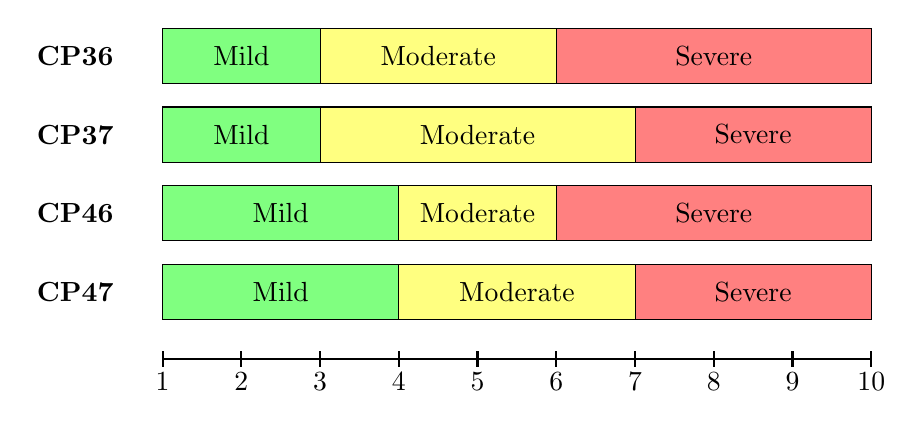
\begin{tikzpicture}
        % Definizione delle coordinate di partenza
        \foreach \y/\name/\mild/\moderate/\severe in {4.5/CP36/3/6/10, 
                                                      3.5/CP37/3/7/10, 
                                                      2.5/CP46/4/6/10, 
                                                      1.5/CP47/4/7/10} {
            % Barre per i livelli di dolore
            \draw[fill=green!50] (1,\y) rectangle (\mild,\y+0.7) node[pos=.5] {Mild};
            \draw[fill=yellow!50] (\mild,\y) rectangle (\moderate,\y+0.7) node[pos=.5] {Moderate};
            \draw[fill=red!50] (\moderate,\y) rectangle (\severe,\y+0.7) node[pos=.5] {Severe};
            % Nome del protocollo
            \node[left] at (0.5,\y+0.35) {\textbf{\name}};
        }
        
        % Scala
        \draw[thick] (1,1) -- (10,1); % Linea di riferimento
        \foreach \x in {1,2,3,4,5,6,7,8,9,10}
            \draw[thick] (\x,0.9) -- (\x,1.1) node[below=4pt] {\x}; % Ticks sulla scala abbassati di 4pt

    \end{tikzpicture}
    \caption{An overview of the protocols and their levels for pain intensity.}
    \label{fig:protocolli_dolore}
\end{figure}

To identify the optimal cut-off configuration that maximizes the separation between pain levels in terms of their impact on multiple functional interference variables, we adopt a data-driven approach based on Multivariate Analysis of Variance (MANOVA) \citep{o1985manova}, inspired by the methodology proposed by \citep{serlin1995cancer}. In the original study, robustness was evaluated across cultural groups using the variable \textit{Nation}, under the assumption that a valid discretization strategy should preserve its discriminative ability independently of population-specific effects. In our setting, we adopt the same principle but consider a demographic factor, namely \textit{Sex}, which is available in all synthetic datasets. Accordingly, we model both the main effect of pain categorization and its interaction with sex, in order to assess whether the discriminative structure induced by each cut-off configuration remains stable across demographic subgroups.

The analysis is conducted by considering the PRI score as the underlying continuous measure of pain intensity, which is first normalized to a 0--10 scale to ensure consistency with standard clinical interpretations. Based on this representation, each patient is assigned to one of three categories, mild, moderate, or severe, according to the selected cut-off protocol. The MANOVA model treats pain category as the independent variable and a set of functional interference measures as multivariate dependent variables. Specifically, we consider seven dimensions capturing the impact of pain on daily life, including \textit{Activity}, \textit{Mood}, \textit{Sleep}, \textit{Work}, \textit{Relate}, \textit{Enjoy}, and \textit{Walk}. These variables represent interrelated aspects of functional impairment and are therefore more appropriately analyzed jointly rather than through separate univariate tests.

To evaluate the effectiveness of each cut-off configuration, we rely on three standard multivariate test statistics, namely Pillai’s trace \citep{dasgupta2005p}, Wilks’ lambda \citep{alrawashdeh2017wilk}, and Hotelling–Lawley trace \citep{dasgupta2005awley}. These criteria provide complementary perspectives on the proportion of explained variance and are commonly transformed into approximate F-statistics for hypothesis testing. Consistency across these measures strengthens the reliability of the conclusions.

The optimal cut-off configuration is selected based on two complementary criteria. First, we consider the magnitude of the multivariate F-statistic associated with the main effect of pain category, under the assumption that higher values indicate stronger separation between groups\citep{tabachnick2007using}. Second, we evaluate the ratio between the F-statistic of the main effect and that of the interaction term, Pain $\times$ Sex, which provides an indication of robustness with respect to demographic variability\citep{maxwell2017designing}. A higher ratio suggests that the discriminative power of the categorization is not substantially affected by sex. In addition to statistical significance, we quantify the explanatory power of each configuration by computing the partial eta squared $\eta^2$, which measures the proportion of variance in the dependent variables explained by the pain categorization and provides an interpretable estimate of effect size \citep{richardson2011eta}.

After selecting the optimal cut-off configuration, we assess whether the resulting pain stratification is associated with a coherent and reliable measurement of functional interference. This step is necessary to validate that the observed effects are not only statistically significant across groups, but also internally consistent across the different dimensions of interference, such as activity, sleep, mood, and work. To this end, we compute Cronbach’s alpha \citep{forero2024cronbach} on the set of interference items within each pain level (mild, moderate, severe), separately for males and females. This analysis evaluates whether the interference variables jointly capture a stable latent construct and whether this structure remains consistent across severity levels.

To further validate the statistical structure of the dataset, we complement the previous analyses with an examination of the association between pain levels and a set of clinical and demographic variables. This step is motivated by the need to verify whether the discretized pain categories are consistent with known or expected patterns of symptom manifestation, and whether the resulting stratification reflects meaningful differences across patient subgroups. To this end, we employ Pearson’s chi-square test to assess the independence between categorical variables. The test evaluates whether the observed frequencies in contingency tables significantly deviate from those expected under the null hypothesis of independence. Formally, the null hypothesis ($H_0$) states that the two variables are independent, whereas the alternative hypothesis ($H_1$) indicates the presence of a statistical association. Thus, demographic characteristics, symptom descriptors, and functional variables are compared across pain levels to identify statistically significant associations and potential trends linked to pain severity. 

An overview of the methodological workflow is summarized in Figure~\ref{fig:pipeline_analysis}.

\begin{figure}[t!]
\centering

\includegraphics[width=.99\linewidth]{images/figure4_horizontal.png}
\caption{Overview of the pipeline for identifying optimal cut-off for the pain intensity.\label{fig:pipeline_analysis}}
\end{figure}

\subsubsection{MANOVA Results Across the \dbsuite suite}

\paragraph{Phase 1: Cut-off Selection via Multivariate F-Statistics}

Across three of the four synthetic datasets, namely \dbGPT, \dbClaude, \dbDeepSeek, and \dbDoctorAI, the cut-off protocol CP47 emerged as the optimal configuration according to both selection criteria: the absolute magnitude of the multivariate F-statistic associated with the main effect of pain level, and the ratio between this statistic and the interaction term F(Pain~$\times$~Sex). In all three cases and across all three multivariate criteria, Pillai's trace, Wilks' lambda, and Hotelling--Lawley trace, CP47 yielded consistently higher F(Pain Level) values and favorable discrimination ratios, indicating that the $[1\text{--}4]$, $[5\text{--}7]$, and $[8\text{--}10]$ thresholds provide the strongest and most demographically robust separation of pain categories in LLM-generated data.

The \dbDoctorAI dataset constitutes a notable exception. In this case, the absolute F-statistics associated with the main effect of pain level are markedly lower across all cut-off configurations, with the maximum observed value remaining below 1.0 for all three multivariate tests. Under these conditions, CP37 was selected as the best-performing protocol based on the highest F(Pain Level) among the alternatives, though the discrimination signal itself is substantially weaker than in the other three datasets. This finding suggests that the DoctorAI-generated data does not produce a well-differentiated multivariate structure across pain levels, regardless of the cut-off scheme adopted, which represents a qualitative difference compared to the outputs of the other three models.

\paragraph{Phase 2: Robustness with Respect to Biological Sex}

A critical criterion for clinical validity of a pain categorization scheme is its stability across demographic subgroups. In the \dbClaude and \dbDeepSeek datasets, the interaction term F(Pain~$\times$~Sex) remains consistently small under the CP47 configuration, yielding high discrimination ratios and suggesting that the chosen cut-off structure is robust with respect to sex. This is particularly relevant for clinical decision support, where a stratification dependent on demographic variables would introduce systematic bias in treatment recommendations.

The Claude-generated dataset exhibits a similar pattern of low interaction values under CP47, resulting in substantially higher ratios compared to the alternative protocols. For instance, the Hotelling--Lawley trace yields a ratio of 165.01 for CP47, versus 53.11 for CP37, reinforcing the superiority of this cut-off in terms of robustness.

The \dbDeepSeek dataset presents a markedly different profile: the interaction term F(Pain~$\times$~Sex) systematically exceeds the main effect F(Pain Level) across all cut-off configurations and all multivariate criteria. The resulting ratios fall below $1.0$ in all cases, indicating that sex accounts for more variance in the interference outcomes than the pain category itself. This structural anomaly suggests that the DoctorAI model may have introduced sex-related patterns that confound the pain-interference relationship, or that the generated data does not faithfully reflect the clinically expected dominance of pain severity over demographic variation.

\paragraph{Phase 3: Effect Size}
The mean partial eta squared, $\overline{\eta^2}$, provides a standardized and interpretable measure of the explanatory power of the selected cut-off configuration. Consistent with the F-statistic findings, substantial differences emerge across models. \dbGPT dataset yields the highest effect size under CP47, $\overline{\eta^2} = 0.90$, closely followed by the \dbDoctorAI dataset under CP37, $\overline{\eta^2} = 0.91$, and the \dbClaude dataset, $\overline{\eta^2} = 0.62$ under CP47. The \dbDeepSeek dataset reports a lower value, $\overline{\eta^2} = 0.75$ under CP47, though still indicative of a large effect. It is important to notice that for the \dbDoctorAI dataset, the high $\overline{\eta^2}$ values should be interpreted with caution, given the anomalous F-statistic structure discussed above: a large proportion of explained variance does not constitute evidence of a valid pain stratification when the interaction term dominates over the main effect. In contrast, for \dbGPT and \dbClaude datasets, the combination of high F(Pain Level), low F(Pain~$\times$~Sex), and elevated $\overline{\eta^2}$ jointly supports the validity of the CP47-based stratification.

\paragraph{Phase 4: Internal Consistency via Cronbach's Alpha}

The reliability analysis performed using Cronbach's alpha on the seven interference items, Activity, Mood, Sleep, Work, Relate, Enjoy, and Walk, stratified by pain level and biological sex, reveals substantial variability across models and further underscores the qualitative differences in data structure.

For the \dbGPT dataset, internal consistency is uniformly excellent across all pain levels and both sexes. Alpha values exceed 0.98 in the mild stratum, remain in the range $0.94$--$0.95$ in the moderate stratum, and stabilize around $0.88$ in the severe stratum. The monotonically decreasing pattern with increasing pain severity, attributable to greater response heterogeneity at higher intensities, is theoretically coherent and indicative of a well-structured latent construct across the full severity range.

The \dbDeepSeek dataset presents a similar, albeit less pronounced, consistency profile. Alpha values are high in the moderate, approximately $0.96$--$0.97$, and severe, approximately $0.82$--$0.83$ categories in both sexes, with a slight divergence in the mild stratum, where the small sample sizes limit the interpretability of the estimates. The consistency between male and female groups is high across moderate and severe pain, with minor differences in the mild stratum, suggesting a degree of sex-related variability in the low-pain range that warrants further investigation in larger samples.

The \dbClaude dataset exhibits a distinctly non-monotonic reliability profile. While alpha values are acceptable in the mild stratum for males, $0.77$, and good to excellent in the severe stratum for both sexes, $0.82$--$0.88$, the moderate stratum yields strongly negative alpha values in both groups, males: $-0.28$, females: $-0.03$. Negative Cronbach's alpha values indicate that the inter-item correlations are predominantly negative, which violates the assumption of essential tau-equivalence and signals a fundamental incoherence in how the interference construct is expressed at moderate pain levels. This pattern may reflect an internal inconsistency in how the Claude model generated responses in the mid-range pain category, potentially encoding contradictory patterns across different interference domains. Importantly, this limitation does not compromise the severe stratum, which shows coherent and clinically interpretable reliability values.

The \dbDoctorAI dataset presents the most severe reliability failure. Cronbach's alpha values are near-zero or negative across all pain levels and both sexes, with no stratum achieving acceptable internal consistency, all values ranging from $-0.38$ to $0.10$. Item-level deletion analysis does not identify any single item whose removal would restore reliability, confirming that the failure is systemic rather than attributable to a single poorly performing variable. These results indicate that the interference items in the DoctorAI-generated data do not co-vary in a coherent manner, suggesting that this model produced statistically independent or even antagonistic response patterns across the seven functional domains.

\paragraph{Overall results} The comparative analysis across the synthetic datasets reveals different characteristics of the generated data across the four models.
\dbGPT dataset demonstrates the most favorable combination of properties: strong multivariate discrimination, negligible demographic interaction, large effect size, excellent cut-off stability, and high internal consistency across all pain levels. These results suggest that this data faithfully replicates the expected psychometric structure of clinical pain instruments, making it a good choice for training and evaluating learning models.

The \dbClaude dataset produces a valid and clinically coherent stratification under CP47, supported by the highest discrimination ratios among all models, but exhibits a pronounced anomaly in the moderate pain stratum, where Cronbach's alpha becomes negative. This suggests that learning models may struggle to evaluate intermediate pain intensities and that results derived from this dataset at the moderate level should be interpreted with caution.

The \dbDeepSeek dataset ranks second in overall validity, showing a clear preference for CP47, robust discrimination ratios, and acceptable internal consistency. Its primary limitation lies in the relatively small sample sizes in the mild pain stratum, which constrain the reliability of alpha estimates at that level.

The \dbDoctorAI dataset diverges from the others across all analytical phases. The F-statistic structure is inverted relative to clinical expectations, with gender interactions dominating over pain-level effects; no cut-off protocol restores an acceptable discrimination profile. Moreover, Cronbach's alpha remains near zero or negative across all levels and subgroups. %Taken together, these findings indicate that the DoctorAI-generated data does not capture the multivariate structure of pain-related functional impairment in a clinically meaningful way, and its use as a training dataset for a decision support system would require substantial preprocessing or should be reconsidered.

This analysis shows that the convergent application of MANOVA cut-off evaluation provides several useful details for benchmarking synthetic clinical data. Moreover, as we have seen, the CP47 appears to be the optimal cut-off across three of four datasets, which lends external validity to this threshold as a generalizable choice for pain categorization in the clinical context studied. The results also suggest that internal reliability, as measured by Cronbach's alpha, constitutes a particularly discriminating criterion: datasets that pass the MANOVA filter may still fail at the reliability level, as shown by the Claude moderate stratum, while datasets that fail at the MANOVA level are also likely to fail at the reliability level, as shown by DoctorAI. Further details about the analysis and scores are shown in the \ref{sec:appendix_manova}.



\section{Word-based Classification of Pain Etiology\label{sec:sec6}}
% \ste{Discutere dei risultati presentati in 5.1.5, 5.2.5, 5.3.5 e 5.4.5 della tesi. La discussione deve essere unica e fatta in parallelo per tutti e 4 i dataset. \hl{NON PARLARE DEI RISULTATI DI CLASSIFICAZIONE, verranno discussi nella RQ1.2}}

To investigate whether linguistic descriptors can discriminate between different pain mechanisms, we adopt a word-based classification framework inspired by \citep{wilkie2001nociceptive}. Figure \ref{fig:word_pipeline_analysis} shows an overview of the structured word-based classification pipeline underlying the analysis of the pain etiology. More specifically, we analyze whether the qualitative descriptors selected by patients can distinguish between nociceptive and neuropathic pain. Pain descriptions are collected using the McGill Pain Questionnaire, which provides a standardized set of 78 descriptors capturing multiple dimensions of pain quality. Moreover, each pain site is independently classified as nociceptive or neuropathic according to clinically grounded criteria defined through the Lung Cancer Etiology Tool (LCET) \citep{wilkie2001nociceptive}, ensuring a reliable reference label for the underlying pain mechanism\footnote{The complete set of criteria used for etiological classification, together with their observed frequency of application in the dataset, is shown in Table~\ref{tab:lcet_criteria}.}.
% Table~\ref{tab:lcet_criteria} reports the complete set of criteria used for etiological classification, together with their observed frequency of application in the dataset.


In the data transformation phase, each descriptor is encoded as a binary variable indicating its presence or absence in the patient’s report. This results in a structured feature matrix where rows correspond to pain sites and columns to descriptors. For instance, a pain site described with the terms \textit{shooting} and \textit{tingling} would be encoded with value 1 for these descriptors and 0 for all others, while a site described with pressing and itchy would have the corresponding binary indicators activated only for those terms.

\begin{figure}[t!]
\centering

\includegraphics[width=.99\linewidth]{images/figure5.png}
\caption{Overview of the pipeline for pain etiology classification. \label{fig:word_pipeline_analysis}}
\end{figure}

Starting from the previous step, we perform a univariate screening step aimed at identifying descriptors significantly associated with pain etiology. For each descriptor, we define a $2 \times 2$ contingency table, and apply Fisher’s exact test to assess whether its frequency differs between nociceptive and neuropathic pain \citep{kim2017statistical}. Descriptors with a $p$-value lower than 0.10 are retained for further analysis, ensuring that only potentially discriminative features are considered. Then, to complement statistical significance, we quantify the strength and direction of association using the Odds Ratio (OR), computed from the same contingency tables computed in the previous step. Under the adopted coding scheme, i.e., rows representing the presence or absence of the descriptor and columns representing the two pain classes (nociceptive vs. neuropathic), OR values greater than 1 indicate a higher prevalence in nociceptive pain, whereas values lower than 1 indicate a higher prevalence in neuropathic pain. This measure provides an interpretable effect size that characterizes the discriminative role of each descriptor. For instance, an OR lower than 1 for the descriptor tingling indicates that this term is more frequently associated with neuropathic pain, whereas an OR greater than 1 for pressing suggests a higher prevalence in nociceptive pain.

The diagnostic relevance of each descriptor is then evaluated through sensitivity, specificity, and positive predictive value (PPV). These metrics, derived from the contingency tables, quantify the ability of each descriptor to correctly identify or exclude a given pain type when considered in isolation. This step allows us to highlight the limitations of single descriptors, which may exhibit high precision but low sensitivity, or vice versa. 

Given the multidimensional nature of pain, the analysis moves to a multivariate modeling phase, where all statistically significant descriptors are jointly considered. Thus, we employ a logistic regression model to capture their combined effect on pain etiology. Each descriptor is considered from the model as a binary predictor, which aims to estimate a coefficient for each term, representing its contribution to the classification task.

Based on the estimated coefficients, a predictive score is computed as a linear combination of the selected descriptors. This formulation arises from the underlying assumption of logistic regression that the \emph{log-odds} of the target variable can be expressed as a linear function of the input features. In particular, modeling the log-odds rather than the probability itself allows the relationship between predictors and outcome to remain linear, while still ensuring a valid probabilistic interpretation. Formally, the predictive score corresponds to the logit transformation of the probability, i.e., the logarithm of the odds of a pain site being neuropathic. This quantity can take any real value, making it suitable for linear modeling without violating the bounded nature of probabilities. To convert this unbounded score into a valid probability in the range $[0,1]$, the logistic (sigmoid) function is applied: $p = \frac{1}{1 + e^{-\text{score}}}$.This transformation is strictly monotonic and maps negative scores to probabilities below $0.5$ and positive scores to probabilities above $0.5$, preserving the ordering induced by the linear predictor. %Moreover, it provides a smooth and differentiable mapping, which is essential for parameter estimation via maximum likelihood.
Finally, in the classification step, we consider a decision threshold set to 0.5, which we apply to assign each pain site to either the neuropathic or nociceptive class. The predicted labels are then compared with the type of pain described in the MPQs to assess overall model performance, enabling a direct evaluation of the multiple descriptors of pain within a unified pain type.




% \paragraph{ChatGPT Dataset} The univariate analysis on the dataset of MPQ generated by ChatGPT identified thirteen descriptors significantly associated with pain etiology at the $p < 0.10$ threshold. Among these, \textit{shooting}, \textit{tingling}, \textit{crushing}, \textit{blinding}, \textit{tight}, and \textit{cold} were selected more frequently for sites categorized as \textit{neuropathic}, while \textit{itchy}, \textit{pressing}, \textit{smarting}, \textit{flashing}, \textit{jumping}, \textit{freezing}, and \textit{tearing} showed higher prevalence in \textit{nociceptive} pain sites. 
% %Table \ref{tab_pain_qualiti} in the Appendix shows all the words analyzed from the considered dataset.

% The diagnostic performance of individual descriptors, summarized in Table \ref{tab:ability_to_predict_gpt}\footnote{The complete evaluation version is available in \ref{sec:app_etiologiogy}.}, shows a clear asymmetry between the two classes. For the prediction of neuropathic pain, shooting and tingling achieve a specificity and positive predictive value of 100\%, indicating that when either term is reported, the classification is virtually certain. However, their low sensitivity values, 58\% and 42\% respectively, indicate that a substantial proportion of neuropathic cases remains undetected. Crushing, tight, and cold display moderate specificity in the range 74--86\% and lower positive predictive values of 68--70\%, reflecting a reduced diagnostic reliability. Blinding shows the weakest specificity among neuropathic predictors, 62\%, and a positive predictive value of 67\%, indicating an elevated risk of false positives. For the prediction of nociceptive pain, jumping achieves the highest sensitivity, 53\%, and a positive predictive value of 62\%, making it the most informative single-term predictor in this class, albeit with a non-negligible error margin. Flashing presents a balanced profile, with sensitivity of 47\% and specificity of 79\%, yielding a positive predictive value of 59\%. Freezing and tearing show the lowest positive predictive values, 48\% and 50\% respectively, suggesting limited standalone diagnostic utility. Subsequently, the descriptors identified as significant are used. Considering the set of 13 words selected to classify pain as nociceptive or neuropathic, a logistic regression model shows that the combination of these descriptors correctly classifies 97.44\% of sites as nociceptive pain and 88.52\% of sites as neuropathic pain, with an overall accuracy of 92\%

% \begin{table}[t!]
% \centering
% \begin{minipage}{0.49\textwidth}
% \centering
% \renewcommand{\arraystretch}{1.135}
% \scalebox{0.7}{
% \small
% \begin{tabular}{clccc}
% \toprule
%     & \textbf{Neuropathic} & \textbf{Sens.} & \textbf{Spec.} & \textbf{PPV} \\
%     \hline
%     \multirow{6}{*}{\rotatebox{90}{ChatGpt}} 
%     & shooting & 58\%  & 100\%  & 100\%  \\
%     & tingling & 42\%  & 100\%  & 100\%  \\
%     & crushing & 22\%  & 86\% & 70\% \\
%     & blinding & 50\% & 62\%  & 67\%  \\
%     & tight & 23\% & 84\%  & 68\%  \\
%     & cold & 36\% & 74\%  & 68\%  \\
%     \midrule
%     \multirow{7}{*}{\rotatebox{90}{Claude}} 
%     & Radiating & 31\% & 98\% & 98\% \\
%     & Spreading & 30\% & 94\% & 93\% \\
%     & Hurting & 23\% & 91\% & 88\% \\
%     & Quivering & 18\% & 92\% & 87\% \\
%     & Stabbing & 23\% & 87\% & 83\% \\
%     & Sharp & 40\% & 72\% & 80\% \\
%     & Tingling & 26\% & 84\% & 82\% \\
%     \midrule
%     \multirow{2}{*}{\rotatebox{90}{Doct.}} 
%     & Intense & 21\% & 89\% & 92\% \\
%     & Freezing & 37\% & 74\% & 89\% \\
%     \bottomrule
% \end{tabular}}
% % \caption{Neuropathic pain descriptors.}
% \end{minipage}
% \hfill
% \begin{minipage}{0.49\textwidth}
% \centering
% \renewcommand{\arraystretch}{1}
% \scalebox{0.7}{
% \small
% \begin{tabular}{clccc}
% \toprule
%     & \textbf{Nociceptive} & \textbf{Sens.} & \textbf{Spec.} & \textbf{PPV} \\
%     \hline
%     \multirow{7}{*}{\rotatebox{90}{ChatGpt}} 
%     & itchy & 39\% & 82\%  & 59\%  \\
%     & pressing & 25\% & 84\%  & 49\%  \\
%     & smarting & 34\% & 81\%  & 53\%  \\
%     & flashing & 47\% & 79\%  & 59\%  \\
%     & jumping & 53\% & 79\%  & 62\%  \\
%     & freezing & 40\%  & 72\%  & 48\%  \\
%     & tearing & 27\%  & 83\%  & 50\%  \\
%     \midrule
%     \multirow{6}{*}{\rotatebox{90}{Claude}} 
%     & Piercing & 55\% & 83\% & 53\% \\
%     & Aching & 33\% & 84\% & 41\% \\
%     & Penetrating & 38\% & 78\% & 38\% \\
%     & Cool & 46\% & 69\% & 34\% \\
%     & Stinging & 36\% & 75\% & 33\% \\
%     & Killing & 25\% & 83\% & 34\% \\
%     \midrule
%     \multirow{4}{*}{\rotatebox{90}{DoctorAI}} 
%     & Cold & 47\% & 68\% & 20\% \\
%     & Quivering & 28\% & 84\% & 23\% \\
%     & Gruelling & 28\% & 84\% & 22\% \\
%     & Pricking & 29\% & 82\% & 21\% \\
%     \bottomrule
% \end{tabular}}
% % \caption{Nociceptive pain descriptors.}
% \end{minipage}
% {\scriptsize {Note: Sens. = Sensitivity; Spec. = Specificity; PPV = Positive Predictive Value.}}
% \caption{Left: Neuropathic pain descriptors. Right: Nociceptive pain descriptors.\label{tab:ability_to_predict_gpt}}
% \end{table}

% When all thirteen significant descriptors are jointly considered within the logistic regression framework, the resulting predictive score is defined as follows:

% \[
% \begin{aligned}
% \text{Predictive Score} =\ & 0.815 + 3.382 \times \text{shooting} + 3.881 \times \text{tingling} + 0.540 \times \text{crushing} \\
% & + 0.729 \times \text{blinding} + 0.171 \times \text{tight} + 0.095 \times \text{cold} \\
% & - 0.721 \times \text{itchy} - 0.827 \times \text{pressing} - 0.777 \times \text{smarting} \\
% & - 1.777 \times \text{flashing} - 1.605 \times \text{jumping} - 0.658 \times \text{freezing} \\
% & - 0.655 \times \text{tearing}
% \end{aligned}
% \]

\section{Experimental evaluation\label{sec:evaluation}}
The experimental evaluation was conducted on the \dbsuite suite datasets generated by the four LLMs considered in the study to analyze their contributions to the classification of intensity and etiology dimensions. At this stage, the analysis is not limited to the performance of supervised models, but also includes a preliminary verification of the internal consistency of the generated datasets, in order to assess whether the categorical structures produced by the models reflect interpretable configurations coherent with the clinical domain of reference.

\subsection{Experimental settings and Evaluation Metrics}
The experimental analysis was carried out separately on each of the synthetic datasets generated by ChatGPT-4, Claude 3.7, DeepSeek R1, and DoctorAI (See Section \ref{sec:dataset_gen}). After the generation and pre-processing phases, each dataset was used to build and evaluate pain classification models according to three distinct perspectives: intensity, etiology, and duration.

\textbf{Feature Configuration.} For the pain intensity classification task, each model was evaluated under two distinct feature configurations. The \textit{All features} configuration employs the complete set of variables derived from the synthetic datasets, including: demographic variables, including \textit{sex}, \textit{age}, and physiological indicators such as \textit{BPM}; numerical scores associated with each of the 19 McGill pain descriptor sub-dimensions, including \textit{Temporal}, \textit{Spatial}, \textit{Punctate Pressure}, \textit{Incisive Pressure}, \textit{Constrictive Pressure}, \textit{Traction Pressure}, \textit{Thermal}, \textit{Brightness}, \textit{Dullness}, \textit{Miscellaneous Sensory}, \textit{Tension}, \textit{Autonomic}, \textit{Fear}, \textit{Punishment}, \textit{Evaluative}, and \textit{Affective}; seven pain interference scores, including \textit{Activity}, \textit{Enjoyment}, \textit{Mood}, \textit{Social Relations}, \textit{Sleep}, \textit{Walking}, \textit{Work}; \textit{temporal pain} pattern, \textit{pain modulation} factors; and additional clinical descriptors, including \textit{surgery site}, \textit{tumor sitology}, \textit{irradiation site}, \textit{osteoarthropathy}, \textit{pain projection}. The \textit{StepWise} (STPWS) configuration applies an automatic forward-stepwise variable selection procedure, which iteratively includes only those features that yield a statistically significant improvement in the predictive performance of the model, thereby reducing dimensionality and mitigating potential multicollinearity effects. This dual evaluation strategy makes it possible to assess both the expressive capacity of the full feature space and the discriminative gain achievable through variable reduction.

\textbf{Target Variable Definition.} For pain intensity classification, three different discretization strategies were considered. The first is based on the \textit{Pain Rating Index} (PRI) expressed on a relative scale; the second on the \textit{Total Pain Score}, also reported on a relative scale; the third adopts a \textit{MANOVA}-driven discretization aimed at identifying the most statistically discriminative cut-offs for distinguishing \textit{mild}, \textit{moderate}, and \textit{severe} levels. Concerning pain etiology and duration, binary formulations were adopted, namely \textit{nociceptive} versus \textit{neuropathic} and \textit{acute} versus \textit{chronic}, respectively.

\textbf{Training and Validation Protocol.} Once the target variables had been defined, each dataset was divided into a training set equal to 80\% and a test set equal to 20\%, while preserving the original class distribution. The models were then trained and compared using a 5-fold cross-validation strategy, in order to improve the stability of the estimates and reduce dependence on a single data partition.

\textbf{Learning Models and Feature Selection.} The models considered in the experimentation include \textit{Logistic Regression}, \textit{Support Vector Machine} (SVM), \textit{XGBoost}, \textit{Bagging}, \textit{CART}, \textit{Random Forest}, and \textit{Na\"{\i}ve Bayes}. Each model was evaluated both by using the entire set of available variables and by employing a subset selected automatically through a \textit{StepWise} procedure, so as to also analyze the contribution of feature selection to the overall discriminative ability.

\textbf{Classification tasks.} The LLM-based evaluation is conducted on the four synthetic datasets of the \dbsuite suite (see Section~\ref{sec:dataset_gen}), each comprising 500~patient records generated by ChatGPT-4, Claude~3.7, DeepSeek~R1, and DoctorAI respectively. Each record contains 20 subscale scores, the corresponding verbal pain descriptors, age, sex, and relevant modulating factors. Two classification tasks are considered: $i$)~\textit{Pain Intensity}, a three-class task (Low / Medium / High) derived from the Pain Rating Index (PRI) according to the relative scoring scheme described in Section~\ref{sec:painscoring}; $ii$)~\textit{Pain Etiology}, a binary task (Nociceptive / Neuropathic) based on the \texttt{pain\_type} variable annotated via the LCET clinical framework (Appendix~\ref{sec:appendix_lcet}).

\textbf{Models.} Eight large-scale LLMs are evaluated, all accessed through the Ollama Cloud API. The evaluated models are: \textbf{Gemma~4~31B}, \textbf{Gemma~3~27B}, \textbf{Gemma~3~12B}, \textbf{Gemma~3~4B}, \textbf{Ministral-3~14B}, \textbf{Ministral-3~8B}, \textbf{Devstral-Small-2~24B}, and \textbf{RNJ-1~8B}. The Gemma~3 family (4B, 12B, 27B parameters) enables a controlled investigation of the effect of parameter count within a single architectural family. The Mistral family (Ministral-3~14B, Ministral-3~8B, Devstral-Small-2~24B) covers a range of instruction-tuned model sizes from the same provider. All models are executed with a decoding temperature of~0 to maximize determinism and ensure exact reproducibility of results.

\textbf{Prompting strategies.} Eight distinct prompting strategies are implemented and empirically evaluated for the Pain Intensity task, and five for the Pain Etiology task, yielding 13 strategy--task combinations overall (see Figure~\ref{fig:prompting} for details). The five strategies applied to Pain Etiology are: Zero-Shot, CoT Simple, CoT Verification, Few-Shot, and Knowledge-Guided. The remaining four (CoT Hierarchical, CoT Ensemble, CoT Decision-Tree, CoT Confidence) are applied to Pain Intensity only.
\begin{itemize}[itemsep=1pt, parsep=1pt, topsep=2pt, leftmargin=10pt]
    \item \textbf{Zero-Shot \citep{ERONEN2022102981}:} the model receives the patient data with a task description only, with no examples or intermediate reasoning steps.
    \item \textbf{CoT Simple \citep{wei2022chain}:} the model is instructed to follow explicit step-by-step reasoning before providing the final classification.
    \item \textbf{CoT Hierarchical \citep{wang2025hcott}:} the model decomposes the reasoning into a hierarchy of clinical sub-questions (e.g., assess each MPQ dimension individually, then integrate) before concluding.
    \item \textbf{CoT Verification \citep{dhuliawala2024chain}:} after producing a first-pass classification, the model is prompted to verify its own answer by checking each reasoning step for consistency.
    \item \textbf{CoT Ensemble \citep{wang2022self}:} the model is asked to produce multiple independent reasoning chains and aggregate them into a final decision.
    \item \textbf{CoT Decision-Tree \citep{yao2023tree}:} the model is guided through a structured decision-tree logic, branching on clinically meaningful thresholds derived from the MPQ scoring rules.
    \item \textbf{CoT Confidence \citep{kadavath2022language}:} the model provides a classification together with an explicit numerical confidence score, and the final label is conditioned on that self-assessed certainty.
    \item \textbf{Few-Shot \citep{brown2020language}:} the model is provided with two in-context labelled examples (one per relevant class) before classifying the target patient.
    \item \textbf{Knowledge-Guided \citep{wang2023self} (Etiology only):} the model is prompted with the predictive formula proposed by~\citep{wilkie2001nociceptive}, based on 13~MPQ descriptors and their associated beta coefficients, and asked to compute the predictive score and derive the classification accordingly.
\end{itemize}

\textbf{Evaluation Metrics.}
To evaluate the predictive performance of the classification models, we adopt a set of standard metrics tailored to the structure of the three supervised tasks considered in this study: $i$) pain intensity classification into mild, moderate, or severe; $ii$) pain etiology classification into nociceptive vs. neuropathic; and $iii$) pain duration classification into acute vs. chronic.

For each task, predictions are evaluated at the level of individual instances, where a True Positive (TP) corresponds to a correctly predicted membership of a sample to a specific clinical class, e.g., correctly identifying a neuropathic pain case, while a True Negative (TN) denotes correct exclusion of a sample from a given class in binary settings, e.g., correctly identifying a nociceptive case as non-neuropathic. False Positives (FP) correspond to instances incorrectly assigned to a target clinical class, e.g., classifying a nociceptive case as neuropathic, whereas False Negatives (FN) represent clinically relevant misclassifications in which a true case of a class, e.g., severe pain, is incorrectly assigned to a lower severity level.

Given the heterogeneous and clinically imbalanced nature of the datasets, particularly in the multi-class intensity setting, all metrics are computed using a macro-averaging strategy, ensuring that each class contributes equally to the final evaluation regardless of its prevalence.
\noindent
The evaluation metrics are defined as follows: Accuracy defined as $\frac{TP + TN}{TP + TN + FP + FN}$, Precision as $\frac{TP}{TP + FP}$, Recall as $\frac{TP}{TP + FN}$, and F1-score as $2 \cdot \frac{Precision \cdot Recall}{Precision + Recall}$.

In the context of this study, macro-averaged precision and recall are particularly relevant, as they measure the ability of the model to correctly identify clinically meaningful but potentially underrepresented classes, such as the \textit{severe} pain category, the \textit{neuropathic} etiology, and the \textit{chronic} pain condition, which are of primary interest in therapeutic decision-making. Accordingly, beyond global Accuracy, special attention is given to class-wise precision and recall for these clinically critical categories, in order to minimize the risk of underdiagnosis in high-impact clinical scenarios.

% \textbf{Classification tasks.} We evaluated the models using a real-world clinical dataset comprising records from nine patients. Each patient record contained 20 subscale scores, the corresponding verbal pain descriptors, age, sex, and relevant modulating factors. Two tasks are considered: $i$) \textit{Pain Intensity:} a three-class classification task (Low / Medium / High) derived from the Pain Rating Index (PRI), calculated as the sum of the 20 McGill Pain Questionnaire (MPQ) subscale scores. Intensity categories are defined according to the relative PRI scoring scheme (Scoring~1) as follows: PRI~$<$~26 (Low), $26 \leq \text{PRI} \leq 45$ (Medium), and PRI~$\geq$~46 (High). \textit{Pain Etiology:} a binary classification task (Nociceptive / Neuropathic) based on the \texttt{pain\_type} variable, which is annotated using the LCET clinical framework described in Appendix~\ref{sec:appendix_lcet}.

% \paragraph{Prompting strategies}
% Four prompting strategies are implemented and evaluated:
% \begin{itemize}[itemsep=1pt, parsep=1pt, topsep=2pt]
%     \item \textbf{Zero-Shot\hl{cite}:} the model receives the patient data with a task description only, with no examples or intermediate reasoning steps.
%     \item \textbf{Chain-of-Thought (CoT):} the model is instructed to follow explicit reasoning steps before providing the final classification.
%     \item \textbf{Few-Shot\hl{cite}:} the model is provided with two in-context labeled examples (one per relevant class) before classifying the target patient.
%     \item \textbf{Knowledge-Guided\hl{cite}} 
% \end{itemize}

% \paragraph{Models}
% % \ste{Da aggiornare con i nuovi risultati}
% % Eight open-weight LLMs, served locally via Ollama, are evaluated:
% % \textbf{Llama 3.2}, \textbf{Mistral 7B}, \textbf{Qwen 2.5 7B}, \textbf{Gemma 2 9B}, \textbf{DeepSeek-R1 7B}, \textbf{Gemma 3 1B}, \textbf{Gemma 3 4B}, and \textbf{Gemma 3 12B}.
% % The Gemma~3 family (1B, 4B, 12B parameters) allows a direct analysis of how parameter scale affects classification reliability within a single architecture family.
% % All models are run at temperature~0 to ensure reproducibility.
% Eleven LLMs are evaluated in total. Eight open-weight models are served locally via Ollama:
% \textbf{Llama~3.2}, \textbf{Mistral~7B}, \textbf{Qwen~2.5~7B}, \textbf{Gemma~2~9B}, \textbf{DeepSeek-R1~7B}, textbf{Gemma~3~1B}, \textbf{Gemma~3~4B}, and \textbf{Gemma~3~12B}. Three additional large-scale models are accessed via the Ollama Cloud API: \textbf{Gemma~4~31B}, \textbf{Ministral~3~8B}, and \textbf{Qwen~3~Next~80B}.
% The Gemma~3 family (1B, 4B, 12B parameters) allows a direct analysis of how parameter scale affects classification reliability within a single architecture family. All models are run at temperature~0 to ensure reproducibility.
% % \textbf{Evaluation Metrics.} To assess the performance of all considered models, we employ four widely established evaluation metrics commonly used in the field of machine learning, i.e., Accuracy, Precision, Recall, and F1-score. These metrics are defined in terms of the number of True Positives (TP), i.e., when an instance of a given pain-related class (e.g., a specific intensity level, etiological category, or duration type) is correctly predicted. Conversely, True Negatives (TN) correspond to instances correctly identified as not belonging to a given class, False Positives (FP) denote instances incorrectly assigned to a class when they actually belong to a different category, and False Negatives (FN) represent instances belonging to a class but incorrectly classified as another category.


% Given the multi-class nature of the considered tasks, including pain intensity (mild, moderate, severe), etiology (nociceptive, neuropathic), and duration (acute, chronic), the evaluation metrics are computed using a macro-averaging strategy across classes, allowing a balanced assessment of model performance across different categories.

% The metrics are formally defined as follows: 

% \ste{TP;TN;FP;FN vanno caratterizzati. Togliere {equation} e mettere inline}

% \begin{equation}
% Accuracy = \frac{TP + TN}{TP + TN + FP + FN}
% \end{equation}

% \begin{equation}
% Precision = \frac{TP}{TP + FP}
% \end{equation}

% \begin{equation}
% Recall = \frac{TP}{TP + FN}
% \end{equation}

% \begin{equation}
% F1\text{-}score = 2 \cdot \frac{Precision \cdot Recall}{Precision + Recall}
% \end{equation}

% In the overall comparison among the datasets generated by the different LLMs, particular attention was devoted to overall accuracy and to the precision achieved on the clinically most critical class, namely the \textit{severe} class for intensity, \textit{neuropathic} for etiology, and \textit{chronic} for duration.


% {\textbf{Statistical Validation}.} Alongside supervised classification, the internal consistency of the synthetic datasets was preliminarily explored through \textit{Multiple Correspondence Analysis} (MCA), with the aim of verifying the presence of interpretable latent dimensions within the generated categorical variables. In addition, for the \textit{word-based} analysis of pain etiology, Fisher’s exact test was employed to identify the most discriminative descriptors, and logistic regression models were used to evaluate their predictive contribution, complementing standard metrics with diagnostic indicators such as \textit{sensitivity}, \textit{specificity}, and \textit{positive predictive value}.

% \section{RQ1: Can predictive models trained on domain-specific questionnaires reliably classify pain-related characteristics, such as intensity, duration, and etiology?}

\section{Multidimensional pain assessment\label{sec:sec8}}
The objective of this evaluation is to investigate whether predictive models trained on data derived from generated domain-specific questionnaires can reliably classify clinical characteristics of pain. The experimental evaluation was performed using synthetic datasets within the \dbsuite, generated by ChatGPT-4, Claude 3.7, DeepSeek R1, and DoctorAI, as detailed in Section \ref{sec:LLM-Based_Synthetic}. Following data generation and preprocessing, each dataset was employed to train and assess machine learning models for the classification of pain intensity and etiology.

\subsection{RQ1: Can predictive models trained on synthetic domain-specific questionnaires reliably classify pain intensity?}

This section evaluates the ability of seven supervised machine learning models to classify pain intensity across the four synthetic datasets of \dbsuite, considering three alternative target variable definitions based on different discretization strategies applied to the McGill Pain Questionnaire scores.

\subsubsection{Classification results considering PRI-based relative scoring}
Table~\ref{tab:scoring_1_model} reports the classification results obtained by the seven learning models evaluated under both feature configurations on each of the four synthetic datasets, using the PRI-based relative scoring as the target variable.

Results are reported per intensity class (see Section \ref{sec:painscoring}), in terms of Precision, Recall, and F1-score, along with overall Accuracy. The Precision–Recall distributions across models and datasets are further visualized in Figure~\ref{fig:plot_scoring1}.

\paragraph{Class-level discriminability}
Across all four datasets and feature configurations, Class~2, i.e., high pain intensity, is consistently classified with near-perfect accuracy, yielding F1-scores that approach or equal $1.00$ in the vast majority of configurations. This result is partly attributable to the higher prevalence of the high-pain group in each dataset: $49.8$\% for \dbGPT, $51.6$\% for \dbClaude, $52.0$\% for \dbDoctorAI, and $69.2$\% for \dbDeepSeek; Table~\ref{tab:pri_class_distribution}, which provides a training signal and reduces the risk of misclassification. In contrast, Class~1 (medium pain intensity) consistently emerges as the most challenging category, exhibiting the lowest F1-scores across all models and datasets and representing the primary source of classification errors. Class~0 (low pain intensity) yields intermediate and more variable results, depending on the specific dataset and model configuration.

\paragraph{Impact of feature selection}
A prominent finding concerns the behavior of the SVM classifier under the two feature configurations. When trained on the full feature set, SVM exhibits a near-complete failure in discriminating one or more intensity classes: F1-score for Class~1 collapses to $0.04$ on \dbGPT, Class~0 is entirely unrecognized (F1~$= 0.00$) on both \dbClaude and \dbDeepSeek, and Class~1 is equally unrecognized on \dbDoctorAI, despite overall Accuracy values of $0.65$--$0.82$, which are inflated by the correct prediction of the dominant Class~2. This degenerate behavior is consistent with the known sensitivity of kernel-based SVMs to high-dimensional, class-imbalanced feature spaces. The application of the STPWS procedure entirely resolves this failure: with the reduced feature subset, SVM achieves competitive performance across all datasets, reaching Accuracy~$= 0.97$ on \dbGPT and Accuracy~$= 0.95$ on \dbClaude. For all remaining models, XGBoost, Bagging, CART, Random Forest, Naïve Bayes, and Logistic Regression, the effect of feature selection is more nuanced: in some cases, the full feature set yields marginally superior results (e.g., Bagging on \dbGPT: Acc~$= 0.95$ vs.\ $0.89$ with STPWS), while in others a comparable or slightly improved performance is obtained with STPWS. These results confirm that stepwise selection is a critical preprocessing step for kernel-based classifiers, whereas ensemble and probabilistic models are comparatively more robust to high-dimensional input.

\paragraph{Dataset-specific results}
On the \dbGPT dataset, the majority of models achieve Accuracy in the range $0.87$--$0.98$ across both feature configurations. Naïve Bayes with all features attains the highest overall Accuracy of $0.98$ (Class~0: P~$= 1.00$, R~$= 0.96$, F1~$= 0.98$; Class~1: F1~$= 0.94$; Class~2: F1~$= 0.99$), followed by Bagging (Acc~$= 0.95$) and XGBoost with STPWS (Acc~$= 0.94$). The Multinomial Logistic Regression (MLR) with STPWS achieves Accuracy~$= 0.96$ with well-balanced performance across all intensity levels (F1: $0.96$/$0.89$/$0.95$ for Class~0/1/2). Similar patterns are observed on \dbClaude, where Naïve Bayes with all features again attains the peak Accuracy of $0.98$ (Class~2: F1~$= 1.00$), and the Multinomial Logistic Regression with STPWS yields Accuracy~$= 0.95$ (F1: $0.97$/$0.91$/$0.96$). On \dbDoctorAI, results are consistent with those obtained on \dbGPT and \dbClaude, with most models achieving an accuracy between $0.88$ and $0.94$. The MLRwith STPWS reaches Accuracy~$= 0.94$ (Class~0: F1~$= 0.96$; Class~1: F1~$= 0.88$; Class~2: F1~$= 0.96$), matched by Random Forest and Naïve Bayes under both feature configurations.

On the \dbDeepSeek dataset, classification performance is substantially lower, particularly for Classes~0 and~1. The marked class imbalance, with $69.2$\% of samples belonging to Class~2, makes accuracy a misleading indicator, as models that trivially predict the dominant class can still achieve Accuracy~$\geq 0.70$. The best-performing configuration, MLRwith STPWS, achieves Accuracy~$= 0.91$ but with F1 scores of only $0.73$ and $0.69$ for Classes~0 and~1, respectively. Class~2 remains near-perfectly classified (F1~$= 0.99$) across all models. This performance gap reflects the limited representation of low- and medium-pain training samples in the \dbDeepSeek dataset, which degrades the model's ability to learn discriminative boundaries for minority intensity levels.

The classification results obtained under the PRI-based scoring scheme indicate that reliable pain intensity recognition is achievable for synthetic datasets generated by \dbGPT, \dbClaude, and \dbDoctorAI, where most models achieve high and balanced performance across the three intensity classes. The STPWS feature selection procedure proves essential for kernel-based models and provides a competitive alternative for interpretability-oriented classifiers. The substantially lower and imbalanced results observed on \dbDeepSeek highlight the critical influence of data generation quality and class distribution on classification accuracy, and suggest that the PRI-based discretization is more sensitive to such distributional properties than other scoring schemes.

% \begin{table}[t!]
% \centering
% \resizebox{\textwidth}{!}{ % Ridimensiona la tabella alla larghezza della pagina
% \begin{tabular}{ll p{2.8 cm} |ccc|ccc|ccc|ccc|c} % p{5cm} permette il ritorno a capo automatico
% \hline
% & \textbf{Modello} & \textbf{Variabili} & \multicolumn{3}{c|}{\textbf{Classe 0}} & \multicolumn{3}{c|}{\textbf{Classe 1}} & \multicolumn{3}{c|}{\textbf{Classe 2}} & \multicolumn{3}{c|}{\textbf{Macro Avg}} & \textbf{Acc.} \\
% \cline{4-6} \cline{7-9} \cline{10-12} \cline{13-15}
% & & & Prec. & Recall & F1 & Prec. & Recall & F1 & Prec. & Recall & F1 & Prec. & Recall & F1 & \\
% \hline
% \multirow{14}{*}{GPT4} & SVM & All features & \g{0.64} & \g{1.00} & \g{0.78} & \g{0.07} & \g{0.05} & \g{0.04} & \g{0.93} & \g{1.00} & \g{0.97} & \g{0.53} & \g{0.67} & \g{0.57} & \g{0.82}  \\
% & SVM & STPWS & \g{0.93} & \g{1.00} & \g{0.96} & \g{0.94} & \g{0.89} & \g{0.91} & \g{1.00} & \g{0.98} & \g{0.99} & \g{0.96} & \g{0.96} & \g{0.96} & \g{0.97}  \\
% & XGBoost & All features    & \g{0.86} & \g{0.96} & \g{0.91} & \g{0.88} & \g{0.78} & \g{0.82} & \g{1.00} & \g{0.98} & \g{0.99} & \g{0.91} & \g{0.91} & \g{0.91} & \g{0.92} \\
% & XGBoost & STPWS    & \g{0.89} & \g{1.00} & \g{0.94} & \g{0.81} & \g{0.72} & \g{0.76} & \g{0.96} & \g{0.95} & \g{0.96} & \g{0.89} & \g{0.89} & \g{0.89} & \g{0.94} \\ 
% & Bagging & All features   & \g{0.89} & \g{0.96} & \g{0.92} & \g{0.88} & \g{0.83} & \g{0.86} & \g{1.00} & \g{0.98} & \g{0.99} & \g{0.92} & \g{0.93} & \g{0.92} & \g{0.95} \\
% & Bagging &  STPWS & \g{0.86} & \g{1.00} & \g{0.93} & \g{0.69} & \g{0.61} & \g{0.65} & \g{0.95} & \g{0.91} & \g{0.93} & \g{0.83} & \g{0.84} & \g{0.83} & \g{0.89} \\
% & CART    &  All variables  & \g{0.77} & \g{0.96} & \g{0.86} & \g{0.73} & \g{0.44} & \g{0.55} & \g{0.95} & \g{0.96} & \g{0.96} & \g{0.82} & \g{0.79} & \g{0.79} & \g{0.87} \\
% & CART    &  STPWS  & \g{0.78} & \g{1.00} & \g{0.88} & \g{0.73} & \g{0.61} & \g{0.67} & \g{1.00} & \g{0.93} & \g{0.96} & \g{0.84} & \g{0.85} & \g{0.84} & \g{0.89} \\
% & Random Forest & All features & \g{0.83} & \g{1.00} & \g{0.91} & \g{1.00} & \g{0.67} & \g{0.80} & \g{0.98} & \g{1.00} & \g{0.99} & \g{0.94} & \g{0.89} & \g{0.90} & \g{0.94} \\
% & Random Forest & STPWS & \g{0.86} & \g{0.96} & \g{0.91} & \g{0.80} & \g{0.67} & \g{0.73} & \g{0.96} & \g{0.96} & \g{0.96} & \g{0.87} & \g{0.86} & \g{0.87} & \g{0.91} \\
% & Naïve Bayes  & All features & \g{1.00} & \g{0.96} & \g{0.98} & \g{0.94}& \g{0.94} & \g{0.94} & \g{0.98} & \g{1.00} & \g{0.99} & \g{0.98} & \g{0.97} & \g{0.97} & \g{0.98} \\
% & Naïve Bayes  & STPWS & \g{1.00} & \g{0.96} & \g{0.85} & \g{0.94} & \g{0.89} & \g{0.98} & \g{0.96} & \g{0.97} & \g{0.92} & \g{0.96} & \g{0.95} & \g{0.95} & \g{0.96} \\ 
% & Logistics multinomial & All features & \g{0.89} & \g{1.00} & \g{0.94} & \g{0.86} & \g{0.67} & \g{0.75} & \g{0.95} & \g{0.96} & \g{0.96} & \g{0.90} & \g{0.88} & \g{0.88} & \g{0.92}  \\
% & {Logistics multinomial} & {STPWS} & \textbf{\g{0.93}} & \textbf{\g{1.00}} & \textbf{\g{0.96}} & \textbf{\g{0.89}} & \textbf{\g{0.89}} & \textbf{\g{0.89}} & \textbf{\g{1.00}} & \textbf{\g{0.96}} & \textbf{\g{0.95}} & \textbf{\g{0.94}} & \textbf{\g{0.95}} & \textbf{\g{0.94}} & \textbf{\g{0.96}} \\ \hline
% \multirow{14}{*}{Claude} & SVM & All features & \g{0.00} & \g{0.00} & \g{0.00} & \g{0.37} & \g{0.36} & \g{0.36} & \g{0.79} & \g{1.00} & \g{0.88} & \g{0.39} & \g{0.45} & \g{0.41} & \g{0.65} \\
% & SVM & STPWS & \g{0.94} & \g{1.00} & \g{0.97} & \g{0.96} & \g{0.93} & \g{0.95} & \g{0.98} & \g{0.98} & \g{0.98} & \g{0.96} & \g{0.97} & \g{0.97} & \g{0.95} \\
% & XGBoost & All features & \g{1.00} & \g{1.00} & \g{1.00} & \g{0.93} & \g{0.96} & \g{0.95} & \g{0.98} & \g{0.96} & \g{0.97} & \g{0.97} & \g{0.98} & \g{0.97} & \g{0.95} \\
% & XGBoost & STPWS & \g{0.89} & \g{1.00} & \g{0.94} & \g{0.96} & \g{0.86} & \g{0.91} & \g{0.96} & \g{0.98} & \g{0.97} & \g{0.94} & \g{0.95} & \g{0.94} & \g{0.95} \\
% & Bagging & All features & \g{0.94} & \g{1.00} & \g{0.97} & \g{0.87} & \g{0.96} & \g{0.92} & \g{1.00} & \g{0.93} & \g{0.96} & \g{0.94} & \g{0.96} & \g{0.95} & \g{0.95} \\
% & Bagging & STPWS & \g{0.94} & \g{1.00} & \g{0.97} & \g{0.84} & \g{0.96} & \g{0.90} & \g{1.00} & \g{0.91} & \g{0.95} & \g{0.93} & \g{0.96} & \g{0.94} & \g{0.94} \\
% & CART & All features & \g{0.89} & \g{1.00} & \g{0.94} & \g{0.96} & \g{0.89} & \g{0.93} & \g{0.98} & \g{0.98} & \g{0.98} & \g{0.95} & \g{0.96} & \g{0.95} & \g{0.94} \\
% & CART & STPWS & \g{0.89} & \g{1.00} & \g{0.94} & \g{0.95} & \g{0.68} & \g{0.79} & \g{0.89} & \g{0.98} & \g{0.93} & \g{0.91} & \g{0.89} & \g{0.89} & \g{0.90} \\
% & Random Forest & All features & \g{0.90} & \g{0.85} & \g{1.00} & \g{0.93} & \g{1.00} & \g{0.97} & \g{1.00} & \g{0.96} & \g{0.98} & \g{0.98} & \g{0.99} & \g{0.98} & \g{0.94} \\
% & Random Forest & STPWS & \g{0.94} & \g{1.00} & \g{0.97} & \g{0.93} & \g{0.89} & \g{0.91} & \g{0.96} & \g{0.96} & \g{0.96} & \g{0.94} & \g{0.95} & \g{0.95} & \g{0.95} \\
% & Naïve Bayes & All features & \g{1.00} & \g{0.88} & \g{0.94} & \g{0.93} & \g{1.00} & \g{0.97} & \g{1.00} & \g{1.00} & \g{1.00} & \g{0.98} & \g{0.96} & \g{0.97} & \g{0.98} \\
% & Naïve Bayes & STPWS & \g{0.94} & \g{0.88} & \g{0.91} & \g{0.93} & \g{0.96} & \g{0.95} & \g{1.00} & \g{1.00} & \g{1.00} & \g{0.96} & \g{0.95} & \g{0.95} & \g{0.97} \\
% & Logistics multinomial & All features & \g{0.83} & \g{0.88} & \g{0.86} & \g{0.88} & \g{0.82} & \g{0.85} & \g{0.96} & \g{0.98} & \g{0.97} & \g{0.89} & \g{0.90} & \g{0.89} & \g{0.92} \\
% & {Logistics multinomial} & {STPWS} & \textbf{\g{0.94}} & \textbf{\g{1.00}} & \textbf{\g{0.97}} & \textbf{\g{0.96}} & \textbf{\g{0.86}} & \textbf{\g{0.91}} & \textbf{\g{0.95}} & \textbf{\g{0.98}} & \textbf{\g{0.96}} & \textbf{\g{0.95}} & \textbf{\g{0.95}} & \textbf{\g{0.95}} & \textbf{\g{0.95}} \\ \hline
% \multirow{14}{*}{DeepSeek} & SVM & All features & \g{0.00} & \g{0.00} & \g{0.00} & \g{0.00} & \g{0.00} & \g{0.00} & \g{0.70} & \g{1.00} & \g{0.82} & \g{0.23} & \g{0.33} & \g{0.27} & \g{0.70} \\
% & SVM & STPWS & \g{1.00} & \g{0.28} & \g{0.43} & \g{0.46} & \g{0.92} & \g{0.61} & \g{0.99} & \g{1.00} & \g{0.99} & \g{0.81} & \g{0.73} & \g{0.68} & \g{0.86} \\
% & XGBoost & All features & \g{1.00} & \g{0.39} & \g{0.56} & \g{0.50} & \g{0.92} & \g{0.65} & \g{0.99} & \g{1.00} & \g{0.99} & \g{0.83} & \g{0.77} & \g{0.73} & \g{0.88} \\
% & XGBoost & STPWS & \g{0.67} & \g{0.33} & \g{0.44} & \g{0.40} & \g{0.67} & \g{0.50} & \g{0.99} & \g{1.00} & \g{0.99} & \g{0.68} & \g{0.67} & \g{0.65} & \g{0.84} \\
% & Bagging & All features & \g{0.90} & \g{0.50} & \g{0.64} & \g{0.53} & \g{0.83} & \g{0.65} & \g{0.99} & \g{1.00} & \g{0.99} & \g{0.80} & \g{0.78} & \g{0.76} & \g{0.89} \\
% & Bagging & STPWS & \g{0.75} & \g{0.67} & \g{0.71} & \g{0.54} & \g{0.58} & \g{0.56} & \g{0.99} & \g{1.00} & \g{0.99} & \g{0.76} & \g{0.75} & \g{0.75} & \g{0.89} \\
% & CART & All features & \g{0.80} & \g{0.44} & \g{0.57} & \g{0.43} & \g{0.75} & \g{0.55} & \g{0.99} & \g{0.97} & \g{0.98} & \g{0.74} & \g{0.72} & \g{0.70} & \g{0.85} \\
% & CART & STPWS & \g{0.50} & \g{0.22} & \g{0.31} & \g{0.32} & \g{0.58} & \g{0.41} & \g{0.99} & \g{0.99} & \g{0.99} & \g{0.60} & \g{0.60} & \g{0.57} & \g{0.80} \\
% & Random Forest & All features & \g{1.00} & \g{0.22} & \g{0.36} & \g{0.44} & \g{0.92} & \g{0.59} & \g{0.99} & \g{1.00} & \g{0.99} & \g{0.81} & \g{0.71} & \g{0.65} & \g{0.85} \\
% & Random Forest & STPWS & \g{0.86} & \g{0.33} & \g{0.48} & \g{0.45} & \g{0.83} & \g{0.59} & \g{0.99} & \g{1.00} & \g{0.99} & \g{0.77} & \g{0.72} & \g{0.69} & \g{0.86} \\
% & Naïve Bayes & All features & \g{0.82} & \g{0.50} & \g{0.62} & \g{0.50} & \g{0.75} & \g{0.60} & \g{0.99} & \g{1.00} & \g{0.99} & \g{0.77} & \g{0.75} & \g{0.74} & \g{0.88} \\
% & Naïve Bayes & STPWS & \g{0.83} & \g{0.56} & \g{0.67} & \g{0.53} & \g{0.75} & \g{0.62} & \g{0.99} & \g{1.00} & \g{0.99} & \g{0.78} & \g{0.77} & \g{0.76} & \g{0.89} \\
% & Logistics multinomial & All features & \g{0.75} & \g{0.33} & \g{0.46} & \g{0.45} & \g{0.83} & \g{0.59} & \g{0.99} & \g{0.99} & \g{0.99} & \g{0.73} & \g{0.72} & \g{0.68} & \g{0.85} \\
% & {Logistics multinomial} & {STPWS} & \textbf{\g{0.92}} & \textbf{\g{0.61}} & \textbf{\g{0.73}} & \textbf{\g{0.59}} & \textbf{\g{0.83}} & \textbf{\g{0.69}} & \textbf{\g{0.99}} & \textbf{\g{1.00}} & \textbf{\g{0.99}} & \textbf{\g{0.83}} & \textbf{\g{0.81}} & \textbf{\g{0.81}} & \textbf{\g{0.91}} \\ \hline
% \multirow{14}{*}{DoctorAI} & SVM & All features & \g{0.61} & \g{0.92} & \g{0.73} & \g{0.00} & \g{0.00} & \g{0.00} & \g{0.87} & \g{1.00} & \g{0.93} & \g{0.49} & \g{0.64} & \g{0.55} & \g{0.75} \\
% & SVM & STPWS & \g{0.96} & \g{0.88} & \g{0.92} & \g{0.83} & \g{0.87} & \g{0.85} & \g{0.96} & \g{0.98} & \g{0.97} & \g{0.92} & \g{0.91} & \g{0.91} & \g{0.93} \\
% & XGBoost & All features & \g{0.85} & \g{0.88} & \g{0.86} & \g{0.78} & \g{0.78} & \g{0.78} & \g{0.98} & \g{0.96} & \g{0.97} & \g{0.87} & \g{0.87} & \g{0.87} & \g{0.90} \\
% & XGBoost & STPWS & \g{0.85} & \g{0.88} & \g{0.86} & \g{0.81} & \g{0.74} & \g{0.77} & \g{0.96} & \g{0.98} & \g{0.97} & \g{0.87} & \g{0.87} & \g{0.87} & \g{0.90} \\
% & Bagging & All features & \g{0.91} & \g{0.84} & \g{0.88} & \g{0.80} & \g{0.87} & \g{0.83} & \g{0.98} & \g{0.98} & \g{0.98} & \g{0.90} & \g{0.90} & \g{0.90} & \g{0.92} \\
% & Bagging & STPWS & \g{0.95} & \g{0.80} & \g{0.87} & \g{0.79} & \g{0.83} & \g{0.81} & \g{0.95} & \g{1.00} & \g{0.97} & \g{0.90} & \g{0.88} & \g{0.88} & \g{0.91} \\
% & CART & All features & \g{0.77} & \g{0.96} & \g{0.86} & \g{0.87} & \g{0.57} & \g{0.68} & \g{0.94} & \g{0.98} & \g{0.96} & \g{0.86} & \g{0.84} & \g{0.83} & \g{0.88} \\
% & CART & STPWS & \g{0.78} & \g{0.84} & \g{0.81} & \g{0.70} & \g{0.61} & \g{0.65} & \g{0.94} & \g{0.96} & \g{0.95} & \g{0.81} & \g{0.80} & \g{0.80} & \g{0.85} \\
% & Random Forest & All features & \g{0.96} & \g{0.92} & \g{0.94} & \g{0.87} & \g{0.87} & \g{0.87} & \g{0.96} & \g{0.98} & \g{0.97} & \g{0.93} & \g{0.92} & \g{0.93} & \g{0.94} \\
% & Random Forest & STPWS & \g{0.92} & \g{0.88} & \g{0.90} & \g{0.87} & \g{0.87} & \g{0.87} & \g{0.98} & \g{1.00} & \g{0.99} & \g{0.92} & \g{0.92} & \g{0.92} & \g{0.94} \\
% & Naïve Bayes & All features & \g{1.00} & \g{0.88} & \g{0.94} & \g{0.79} & \g{1.00} & \g{0.88} & \g{1.00} & \g{0.94} & \g{0.97} & \g{0.93} & \g{0.94} & \g{0.93} & \g{0.94} \\
% & Naïve Bayes & STPWS & \g{1.00} & \g{0.88} & \g{0.94} & \g{0.81} & \g{0.96} & \g{0.88} & \g{0.98} & \g{0.96} & \g{0.97} & \g{0.93} & \g{0.93} & \g{0.93} & \g{0.94} \\
% & Logistics multinomial & All features & \g{0.88} & \g{0.92} & \g{0.90} & \g{0.85} & \g{0.74} & \g{0.79} & \g{0.94} & \g{0.98} & \g{0.96} & \g{0.89} & \g{0.88} & \g{0.88} & \g{0.91} \\
% & {Logistics multinomial} & {STPWS} & \textbf{\g{1.00}} & \textbf{\g{0.92}} & \textbf{\g{0.96}} & \textbf{\g{0.84}} & \textbf{\g{0.91}} & \textbf{\g{0.88}} & \textbf{\g{0.96}} & \textbf{\g{0.96}} & \textbf{\g{0.96}} & \textbf{\g{0.93}} & \textbf{\g{0.93}} & \textbf{\g{0.93}} & \textbf{\g{0.94}} \\
% \hline
%     \end{tabular}
%     }
%     \caption{Classification results considering PRI-based relative scoring. \ste{Da discutere nel primo sottoparagrafo della RQ1.1}}
%     \label{tab:scoring_1_model}
% \end{table}

\begin{table}[t!]
\centering
\resizebox{\textwidth}{!}{ % Ridimensiona la tabella alla larghezza della pagina
\begin{tabular}{ll p{2.8 cm} |ccc|ccc|ccc|c} 
\hline
\textbf{} & \textbf{Model} & \textbf{Features} & \multicolumn{3}{c|}{\textbf{Low: PRI $< 26$}} & \multicolumn{3}{c|}{\textbf{Medium: $26 \leq \text{PRI} \leq 46$}} & \multicolumn{3}{c|}{\textbf{High: $\text{PRI} > 46$}} & \textbf{Acc.} \\
\cline{4-6} \cline{7-9} \cline{10-12}
& & & \textbf{Prec}. & \textbf{Recall} & \textbf{F1} & \textbf{Prec}. & \textbf{Recall} & \textbf{F1} & \textbf{Prec}. & \textbf{Recall} & \textbf{F1} & \\
\hline
\multirow{14}{*}{\rotatebox{90}{\dbGPT}} & SVM & All features & \g{0.64} & \g{1.00} & \g{0.78} & \g{0.07} & \g{0.05} & \g{0.04} & \g{0.93} & \g{1.00} & \g{0.97} & \g{0.82}  \\
& SVM & STPWS & \g{0.93} & \g{1.00} & \g{0.96} & \g{0.94} & \g{0.89} & \g{0.91} & \g{1.00} & \g{0.98} & \g{0.99} & \g{0.97}  \\
& XGBoost & All features    & \g{0.86} & \g{0.96} & \g{0.91} & \g{0.88} & \g{0.78} & \g{0.82} & \g{1.00} & \g{0.98} & \g{0.99} & \g{0.92} \\
& XGBoost & STPWS    & \g{0.89} & \g{1.00} & \g{0.94} & \g{0.81} & \g{0.72} & \g{0.76} & \g{0.96} & \g{0.95} & \g{0.96} & \g{0.94} \\ 
& Bagging & All features   & \g{0.89} & \g{0.96} & \g{0.92} & \g{0.88} & \g{0.83} & \g{0.86} & \g{1.00} & \g{0.98} & \g{0.99} & \g{0.95} \\
& Bagging &  STPWS & \g{0.86} & \g{1.00} & \g{0.93} & \g{0.69} & \g{0.61} & \g{0.65} & \g{0.95} & \g{0.91} & \g{0.93} & \g{0.89} \\
& CART     &  All variables  & \g{0.77} & \g{0.96} & \g{0.86} & \g{0.73} & \g{0.44} & \g{0.55} & \g{0.95} & \g{0.96} & \g{0.96} & \g{0.87} \\
& CART     &  STPWS  & \g{0.78} & \g{1.00} & \g{0.88} & \g{0.73} & \g{0.61} & \g{0.67} & \g{1.00} & \g{0.93} & \g{0.96} & \g{0.89} \\
& Random Forest & All features & \g{0.83} & \g{1.00} & \g{0.91} & \g{1.00} & \g{0.67} & \g{0.80} & \g{0.98} & \g{1.00} & \g{0.99} & \g{0.94} \\
& Random Forest & STPWS & \g{0.86} & \g{0.96} & \g{0.91} & \g{0.80} & \g{0.67} & \g{0.73} & \g{0.96} & \g{0.96} & \g{0.96} & \g{0.91} \\
& Naïve Bayes  & All features & \g{1.00} & \g{0.96} & \g{0.98} & \g{0.94}& \g{0.94} & \g{0.94} & \g{0.98} & \g{1.00} & \g{0.99} & \g{0.98} \\
& Naïve Bayes  & STPWS & \g{1.00} & \g{0.96} & \g{0.85} & \g{0.94} & \g{0.89} & \g{0.98} & \g{0.96} & \g{0.97} & \g{0.92} & \g{0.96} \\ 
& Logistics multinomial & All features & \g{0.89} & \g{1.00} & \g{0.94} & \g{0.86} & \g{0.67} & \g{0.75} & \g{0.95} & \g{0.96} & \g{0.96} & \g{0.92}  \\
& {Logistics multinomial} & {STPWS} & \textbf{\g{0.93}} & \textbf{\g{1.00}} & \textbf{\g{0.96}} & \textbf{\g{0.89}} & \textbf{\g{0.89}} & \textbf{\g{0.89}} & \textbf{\g{1.00}} & \textbf{\g{0.96}} & \textbf{\g{0.95}} & \textbf{\g{0.96}} \\ \hline
\multirow{14}{*}{\rotatebox{90}{\dbClaude}} & SVM & All features & \g{0.00} & \g{0.00} & \g{0.00} & \g{0.37} & \g{0.36} & \g{0.36} & \g{0.79} & \g{1.00} & \g{0.88} & \g{0.65} \\
& SVM & STPWS & \g{0.94} & \g{1.00} & \g{0.97} & \g{0.96} & \g{0.93} & \g{0.95} & \g{0.98} & \g{0.98} & \g{0.98} & \g{0.95} \\
& XGBoost & All features & \g{1.00} & \g{1.00} & \g{1.00} & \g{0.93} & \g{0.96} & \g{0.95} & \g{0.98} & \g{0.96} & \g{0.97} & \g{0.95} \\
& XGBoost & STPWS & \g{0.89} & \g{1.00} & \g{0.94} & \g{0.96} & \g{0.86} & \g{0.91} & \g{0.96} & \g{0.98} & \g{0.97} & \g{0.95} \\
& Bagging & All features & \g{0.94} & \g{1.00} & \g{0.97} & \g{0.87} & \g{0.96} & \g{0.92} & \g{1.00} & \g{0.93} & \g{0.96} & \g{0.95} \\
& Bagging & STPWS & \g{0.94} & \g{1.00} & \g{0.97} & \g{0.84} & \g{0.96} & \g{0.90} & \g{1.00} & \g{0.91} & \g{0.95} & \g{0.94} \\
& CART & All features & \g{0.89} & \g{1.00} & \g{0.94} & \g{0.96} & \g{0.89} & \g{0.93} & \g{0.98} & \g{0.98} & \g{0.98} & \g{0.94} \\
& CART & STPWS & \g{0.89} & \g{1.00} & \g{0.94} & \g{0.95} & \g{0.68} & \g{0.79} & \g{0.89} & \g{0.98} & \g{0.93} & \g{0.90} \\
& Random Forest & All features & \g{0.90} & \g{0.85} & \g{1.00} & \g{0.93} & \g{1.00} & \g{0.97} & \g{1.00} & \g{0.96} & \g{0.98} & \g{0.94} \\
& Random Forest & STPWS & \g{0.94} & \g{1.00} & \g{0.97} & \g{0.93} & \g{0.89} & \g{0.91} & \g{0.96} & \g{0.96} & \g{0.96} & \g{0.95} \\
& Naïve Bayes & All features & \g{1.00} & \g{0.88} & \g{0.94} & \g{0.93} & \g{1.00} & \g{0.97} & \g{1.00} & \g{1.00} & \g{1.00} & \g{0.98} \\
& Naïve Bayes & STPWS & \g{0.94} & \g{0.88} & \g{0.91} & \g{0.93} & \g{0.96} & \g{0.95} & \g{1.00} & \g{1.00} & \g{1.00} & \g{0.97} \\
& Logistics multinomial & All features & \g{0.83} & \g{0.88} & \g{0.86} & \g{0.88} & \g{0.82} & \g{0.85} & \g{0.96} & \g{0.98} & \g{0.97} & \g{0.92} \\
& {Logistics multinomial} & {STPWS} & \textbf{\g{0.94}} & \textbf{\g{1.00}} & \textbf{\g{0.97}} & \textbf{\g{0.96}} & \textbf{\g{0.86}} & \textbf{\g{0.91}} & \textbf{\g{0.95}} & \textbf{\g{0.98}} & \textbf{\g{0.96}} & \textbf{\g{0.95}} \\ \hline
\multirow{14}{*}{\rotatebox{90}{\dbDeepSeek}} & SVM & All features & \g{0.00} & \g{0.00} & \g{0.00} & \g{0.00} & \g{0.00} & \g{0.00} & \g{0.70} & \g{1.00} & \g{0.82} & \g{0.70} \\
& SVM & STPWS & \g{1.00} & \g{0.28} & \g{0.43} & \g{0.46} & \g{0.92} & \g{0.61} & \g{0.99} & \g{1.00} & \g{0.99} & \g{0.86} \\
& XGBoost & All features & \g{1.00} & \g{0.39} & \g{0.56} & \g{0.50} & \g{0.92} & \g{0.65} & \g{0.99} & \g{1.00} & \g{0.99} & \g{0.88} \\
& XGBoost & STPWS & \g{0.67} & \g{0.33} & \g{0.44} & \g{0.40} & \g{0.67} & \g{0.50} & \g{0.99} & \g{1.00} & \g{0.99} & \g{0.84} \\
& Bagging & All features & \g{0.90} & \g{0.50} & \g{0.64} & \g{0.53} & \g{0.83} & \g{0.65} & \g{0.99} & \g{1.00} & \g{0.99} & \g{0.89} \\
& Bagging & STPWS & \g{0.75} & \g{0.67} & \g{0.71} & \g{0.54} & \g{0.58} & \g{0.56} & \g{0.99} & \g{1.00} & \g{0.99} & \g{0.89} \\
& CART & All features & \g{0.80} & \g{0.44} & \g{0.57} & \g{0.43} & \g{0.75} & \g{0.55} & \g{0.99} & \g{0.97} & \g{0.98} & \g{0.85} \\
& CART & STPWS & \g{0.50} & \g{0.22} & \g{0.31} & \g{0.32} & \g{0.58} & \g{0.41} & \g{0.99} & \g{0.99} & \g{0.99} & \g{0.80} \\
& Random Forest & All features & \g{1.00} & \g{0.22} & \g{0.36} & \g{0.44} & \g{0.92} & \g{0.59} & \g{0.99} & \g{1.00} & \g{0.99} & \g{0.85} \\
& Random Forest & STPWS & \g{0.86} & \g{0.33} & \g{0.48} & \g{0.45} & \g{0.83} & \g{0.59} & \g{0.99} & \g{1.00} & \g{0.99} & \g{0.86} \\
& Naïve Bayes & All features & \g{0.82} & \g{0.50} & \g{0.62} & \g{0.50} & \g{0.75} & \g{0.60} & \g{0.99} & \g{1.00} & \g{0.99} & \g{0.88} \\
& Naïve Bayes & STPWS & \g{0.83} & \g{0.56} & \g{0.67} & \g{0.53} & \g{0.75} & \g{0.62} & \g{0.99} & \g{1.00} & \g{0.99} & \g{0.89} \\
& Logistics multinomial & All features & \g{0.75} & \g{0.33} & \g{0.46} & \g{0.45} & \g{0.83} & \g{0.59} & \g{0.99} & \g{0.99} & \g{0.99} & \g{0.85} \\
& {Logistics multinomial} & {STPWS} & \textbf{\g{0.92}} & \textbf{\g{0.61}} & \textbf{\g{0.73}} & \textbf{\g{0.59}} & \textbf{\g{0.83}} & \textbf{\g{0.69}} & \textbf{\g{0.99}} & \textbf{\g{1.00}} & \textbf{\g{0.99}} & \textbf{\g{0.91}} \\ \hline
\multirow{14}{*}{\rotatebox{90}{\dbDoctorAI}} & SVM & All features & \g{0.61} & \g{0.92} & \g{0.73} & \g{0.00} & \g{0.00} & \g{0.00} & \g{0.87} & \g{1.00} & \g{0.93} & \g{0.75} \\
& SVM & STPWS & \g{0.96} & \g{0.88} & \g{0.92} & \g{0.83} & \g{0.87} & \g{0.85} & \g{0.96} & \g{0.98} & \g{0.97} & \g{0.93} \\
& XGBoost & All features & \g{0.85} & \g{0.88} & \g{0.86} & \g{0.78} & \g{0.78} & \g{0.78} & \g{0.98} & \g{0.96} & \g{0.97} & \g{0.90} \\
& XGBoost & STPWS & \g{0.85} & \g{0.88} & \g{0.86} & \g{0.81} & \g{0.74} & \g{0.77} & \g{0.96} & \g{0.98} & \g{0.97} & \g{0.90} \\
& Bagging & All features & \g{0.91} & \g{0.84} & \g{0.88} & \g{0.80} & \g{0.87} & \g{0.83} & \g{0.98} & \g{0.98} & \g{0.98} & \g{0.92} \\
& Bagging & STPWS & \g{0.95} & \g{0.80} & \g{0.87} & \g{0.79} & \g{0.83} & \g{0.81} & \g{0.95} & \g{1.00} & \g{0.97} & \g{0.91} \\
& CART & All features & \g{0.77} & \g{0.96} & \g{0.86} & \g{0.87} & \g{0.57} & \g{0.68} & \g{0.94} & \g{0.98} & \g{0.96} & \g{0.88} \\
& CART & STPWS & \g{0.78} & \g{0.84} & \g{0.81} & \g{0.70} & \g{0.61} & \g{0.65} & \g{0.94} & \g{0.96} & \g{0.95} & \g{0.85} \\
& Random Forest & All features & \g{0.96} & \g{0.92} & \g{0.94} & \g{0.87} & \g{0.87} & \g{0.87} & \g{0.96} & \g{0.98} & \g{0.97} & \g{0.94} \\
& Random Forest & STPWS & \g{0.92} & \g{0.88} & \g{0.90} & \g{0.87} & \g{0.87} & \g{0.87} & \g{0.98} & \g{1.00} & \g{0.99} & \g{0.94} \\
& Naïve Bayes & All features & \g{1.00} & \g{0.88} & \g{0.94} & \g{0.79} & \g{1.00} & \g{0.88} & \g{1.00} & \g{0.94} & \g{0.97} & \g{0.94} \\
& Naïve Bayes & STPWS & \g{1.00} & \g{0.88} & \g{0.94} & \g{0.81} & \g{0.96} & \g{0.88} & \g{0.98} & \g{0.96} & \g{0.97} & \g{0.94} \\
& Logistics multinomial & All features & \g{0.88} & \g{0.92} & \g{0.90} & \g{0.85} & \g{0.74} & \g{0.79} & \g{0.94} & \g{0.98} & \g{0.96} & \g{0.91} \\
& {Logistics multinomial} & {STPWS} & \textbf{\g{1.00}} & \textbf{\g{0.92}} & \textbf{\g{0.96}} & \textbf{\g{0.84}} & \textbf{\g{0.91}} & \textbf{\g{0.88}} & \textbf{\g{0.96}} & \textbf{\g{0.96}} & \textbf{\g{0.96}} & \textbf{\g{0.94}} \\
\hline
    \end{tabular}
    }
    \caption{Classification results considering PRI-based relative scoring.}
    \label{tab:scoring_1_model}
\end{table}

\begin{figure*}[t!]
\centering

\includegraphics[width=\linewidth]{images/pr_diagram_llms_legend.pdf}

\includegraphics[width=.8\linewidth]{images/pr_diagram_llms_2_2_scoring1.pdf}
\caption{Precision and Recall values considering PRI-based relative scoring (Table \ref{tab:scoring_1_model}).\label{fig:plot_scoring1}}
\end{figure*}

\subsubsection{Classification results considering Total Pain Score}

Table~\ref{tab:scoring_2_complete} reports the classification results obtained by all models under both feature configurations, using the Total Pain Score-based discretization as the target variable. Results are reported for Class~0 (low: total score~$< 65$), Class~1 (medium: $65 \leq \text{total} < 91$), and Class~2 (high: total~$\geq 91$), along with overall Accuracy. The corresponding Precision–Recall distributions are visualized in Figure~\ref{fig:plot_scoring2}.

\paragraph{Class distribution and contrast with PRI-based scoring}
The Total Pain Score produces substantially different class distributions compared to the PRI-based scheme (see Table~\ref{tab:total_class_distribution}). For \dbGPT, Class~0 (low pain) is now the dominant group ($48.6$\%), while Class~2 (high pain) constitutes only $14.0$\% of the data, an inversion with respect to the PRI-based distribution where Class~2 accounted for $49.8$\%. For \dbClaude, Class~0 remains the largest group ($43.2$\%). In contrast, \dbDeepSeek now exhibits a nearly balanced three-class distribution ($30.0$\% / $40.0$\% / $30.0$\%), a sharp improvement over the severely imbalanced PRI-based partition ($13.2$\% / $17.6$\% / $69.2$\%). \dbDoctorAI also shows a relatively balanced distribution ($38.4$\% / $25.9$\% / $35.7$\%). 
% These distributional changes alter the classification difficulty profile and directly influence model behavior, most notably for SVM.

% \paragraph{SVM behavior under the Total Pain Score scheme}
% A salient finding is the absence of the degenerate SVM behavior observed under the PRI-based scheme. Under the total score discretization, SVM with all features yields competitive performance across all datasets, including Accuracy~$= 0.93$ on both \dbGPT and \dbClaude, Accuracy~$= 0.79$ on \dbDeepSeek, and Accuracy~$= 0.97$ on \dbDoctorAI, where it constitutes the best-performing configuration. This behavioral recovery confirms that the SVM pathology previously documented was driven by the structural properties of the PRI-based feature-class relationship and is not intrinsic to the classifier. Under the total score scheme, the STPWS procedure no longer provides a systematic advantage: in several cases, the All features configuration equals or outperforms the stepwise-reduced variant (e.g., Logistic Regression on \dbDeepSeek: Acc~$= 0.87$ vs.\ $0.78$ with STPWS; SVM on \dbDoctorAI: Acc~$= 0.97$ vs.\ $0.95$).

\paragraph{Dataset-specific results}
On \dbGPT, the majority of models achieve an accuracy between $0.79$ and $0.96$. The MLRwith all features attains the best performance (Acc~$= 0.96$; Class~0: F1~$= 0.97$; Class~1: F1~$= 0.88$; Class~2: F1~$= 0.96$), despite Class~2 being the minority group ($14.0$\%). CART with all features yields the lowest accuracy (Acc~$= 0.79$), primarily due to poor discrimination of Class~1 (F1~$= 0.46$). On \dbClaude, results are comparable: SVM with all features and MLRwith all features both achieve Accuracy~$= 0.93$, while CART again records the weakest performance (Acc~$= 0.76$; Class~1: F1~$= 0.56$). The Random Forest and Naïve Bayes models yield an accuracy of $0.87$--$0.92$ across both configurations.

On \dbDeepSeek, the now-balanced class distribution yields a more uniform classification difficulty, yet overall performance remains the lowest among all datasets, with Accuracy ranging from $0.72$ to $0.87$. The MLRwith all features is the best configuration (Acc~$= 0.87$), achieving F1~$= 0.94$ for Class~0 and F1~$= 0.87$ for Class~2, while Class~1 (medium, the largest group at $40.0$\%) is the hardest to discriminate (F1~$= 0.72$). STPWS reduces performance significantly for this dataset, suggesting that the informative signal is distributed across the full feature set rather than concentrated in a sparse subset.

On \dbDoctorAI, the total score scheme yields the highest and most uniform results across all four datasets. SVM with all features achieves Accuracy~$= 0.97$ (Class~0: F1~$= 0.99$; Class~1: F1~$= 0.94$; Class~2: F1~$= 0.97$), matched by Naïve Bayes with all features (Acc~$= 0.97$). All remaining models achieve an accuracy between $0.91$ and $0.96$, with Class~1 (medium, $25.9$\%) being the only class with F1-scores occasionally dropping to $0.85$--$0.90$ in CART and STPWS configurations.

The Total Pain Score-based discretization resolves the SVM failure observed under the PRI-based scheme and yields more balanced class distributions, particularly for \dbDeepSeek. \dbDoctorAI emerges as the most accurately classified dataset under this scheme, with most models reaching Accuracy~$\geq 0.94$. The STPWS feature selection procedure provides limited or no benefit under this scoring strategy, suggesting that the total score feature space is inherently well-structured for standard classifiers. \dbDeepSeek and \dbClaude remain the most challenging datasets, with Class~1 (medium pain) consistently representing the primary source of prediction errors.

% \begin{table}[t!]
% \centering
% \resizebox{\textwidth}{!}{ % Ridimensiona la tabella alla larghezza della pagina
% \begin{tabular}{ll p{2.8 cm} |ccc|ccc|ccc|ccc|c} % p{5cm} permette il ritorno a capo automatico
% \hline
% & \textbf{Modello} & \textbf{Variabili} & \multicolumn{3}{c|}{\textbf{Classe 0}} & \multicolumn{3}{c|}{\textbf{Classe 1}} & \multicolumn{3}{c|}{\textbf{Classe 2}} & \multicolumn{3}{c|}{\textbf{Macro Avg}} & \textbf{Acc.} \\
% \cline{4-6} \cline{7-9} \cline{10-12} \cline{13-15}
% & & & Prec. & Recall & F1 & Prec. & Recall & F1 & Prec. & Recall & F1 & Prec. & Recall & F1 & \\
% \hline
%         \multirow{14}{*}{GPT4} & SVM & All features & \g{0.97} & \g{0.97} & \g{0.97} & \g{0.82} & \g{0.78} & \g{0.80} & \g{0.93} & \g{0.96} & \g{0.95} & \g{0.91} & \g{0.90} & \g{0.91} & \g{0.93} \\
%         & SVM & STPWS & \g{0.95} & \g{0.95} & \g{0.95} & \g{0.72} & \g{0.72} & \g{0.72} & \g{0.93} & \g{0.93} & \g{0.93} & \g{0.87} & \g{0.87} & \g{0.87} & \g{0.90} \\
%         & XGBoost & All features & \g{0.97} & \g{0.92} & \g{0.94} & \g{0.64} & \g{0.78} & \g{0.70} & \g{0.93} & \g{0.89} & \g{0.91} & \g{0.85} & \g{0.86} & \g{0.85} & \g{0.88} \\
%         & XGBoost & STPWS & \g{0.94} & \g{0.92} & \g{0.93} & \g{0.54} & \g{0.72} & \g{0.62} & \g{0.93} & \g{0.82} & \g{0.87} & \g{0.80} & \g{0.82} & \g{0.81} & \g{0.84} \\
%         & Bagging & All features & \g{0.92} & \g{0.92} & \g{0.92} & \g{0.65} & \g{0.83} & \g{0.73} & \g{1.00} & \g{0.89} & \g{0.94} & \g{0.86} & \g{0.88} & \g{0.86} & \g{0.89} \\
%         & Bagging & STPWS & \g{0.92} & \g{0.95} & \g{0.93} & \g{0.80} & \g{0.67} & \g{0.73} & \g{0.91} & \g{0.96} & \g{0.93} & \g{0.88} & \g{0.86} & \g{0.87} & \g{0.90} \\
%         & CART & All features & \g{0.95} & \g{0.97} & \g{0.96} & \g{0.43} & \g{0.50} & \g{0.46} & \g{0.83} & \g{0.76} & \g{0.79} & \g{0.74} & \g{0.74} & \g{0.74} & \g{0.79} \\
%         & CART & STPWS & \g{0.92} & \g{0.95} & \g{0.93} & \g{0.54} & \g{0.72} & \g{0.62} & \g{0.87} & \g{0.73} & \g{0.80} & \g{0.78} & \g{0.80} & \g{0.78} & \g{0.81} \\
%         & Random Forest & All features & \g{0.97} & \g{0.95} & \g{0.96} & \g{0.76} & \g{0.72} & \g{0.74} & \g{0.91} & \g{0.96} & \g{0.93} & \g{0.88} & \g{0.87} & \g{0.88} & \g{0.91} \\
%         & Random Forest & STPWS & \g{0.95} & \g{0.95} & \g{0.95} & \g{0.67} & \g{0.67} & \g{0.67} & \g{0.91} & \g{0.91} & \g{0.91} & \g{0.84} & \g{0.84} & \g{0.84} & \g{0.88} \\
%         & Naïve Bayes & All features & \g{0.97} & \g{0.89} & \g{0.93} & \g{0.74} & \g{0.78} & \g{0.76} & \g{0.94} & \g{0.98} & \g{0.96} & \g{0.88} & \g{0.88} & \g{0.88} & \g{0.91} \\
%         & Naïve Bayes & STPWS & \g{0.97} & \g{0.89} & \g{0.93} & \g{0.75} & \g{0.83} & \g{0.79} & \g{0.96} & \g{0.98} & \g{0.97} & \g{0.89} & \g{0.90} & \g{0.90} & \g{0.92} \\
%         & {MLR} & {All features} & \textbf{\g{0.97}} & \textbf{\g{0.97}} & \textbf{\g{0.97}} & \textbf{\g{0.94}} & \textbf{\g{0.83}} & \textbf{\g{0.88}} & \textbf{\g{0.96}} & \textbf{\g{1.00}} & \textbf{\g{0.96}} & \textbf{\g{0.96}} & \textbf{\g{0.94}} & \textbf{\g{0.94}} & \textbf{\g{0.96}} \\
%         & MLR & STPWS & \g{0.97} & \g{0.97} & \g{0.97} & \g{0.76} & \g{0.89} & \g{0.82} & \g{0.98} & \g{0.91} & \g{0.94} & \g{0.90} & \g{0.92} & \g{0.91} & \g{0.93} \\
% \hline
%         \multirow{14}{*}{Claude} & SVM & All features & \g{1.00} & \g{0.93} & \g{0.96} & \g{0.85} & \g{0.88} & \g{0.87} & \g{0.91} & \g{0.97} & \g{0.94} & \g{0.92} & \g{0.93} & \g{0.92} & \g{0.93} \\
%         & SVM & STPWS & \g{1.00} & \g{0.90} & \g{0.95} & \g{0.82} & \g{0.88} & \g{0.85} & \g{0.91} & \g{0.97} & \g{0.94} & \g{0.91} & \g{0.92} & \g{0.91} & \g{0.92} \\
%         & XGBoost & All features & \g{0.95} & \g{0.90} & \g{0.93} & \g{0.79} & \g{0.85} & \g{0.81} & \g{0.94} & \g{0.94} & \g{0.94} & \g{0.89} & \g{0.90} & \g{0.89} & \g{0.90} \\
%         & XGBoost & STPWS & \g{0.95} & \g{0.86} & \g{0.90} & \g{0.72} & \g{0.81} & \g{0.76} & \g{0.91} & \g{0.94} & \g{0.92} & \g{0.86} & \g{0.87} & \g{0.86} & \g{0.87} \\
%         & Bagging & All features & \g{0.93} & \g{0.93} & \g{0.93} & \g{0.72} & \g{0.81} & \g{0.76} & \g{0.93} & \g{0.84} & \g{0.89} & \g{0.86} & \g{0.86} & \g{0.86} & \g{0.87} \\
%         & Bagging & STPWS & \g{0.88} & \g{0.90} & \g{0.89} & \g{0.71} & \g{0.65} & \g{0.68} & \g{0.88} & \g{0.91} & \g{0.89} & \g{0.82} & \g{0.82} & \g{0.82} & \g{0.84} \\
%         & CART & All features & \g{0.83} & \g{0.83} & \g{0.83} & \g{0.54} & \g{0.58} & \g{0.56} & \g{0.87} & \g{0.81} & \g{0.84} & \g{0.75} & \g{0.74} & \g{0.74} & \g{0.76} \\
%         & CART & STPWS & \g{0.88} & \g{0.88} & \g{0.88} & \g{0.63} & \g{0.65} & \g{0.64} & \g{0.87} & \g{0.84} & \g{0.86} & \g{0.79} & \g{0.79} & \g{0.79} & \g{0.81} \\
%         & Random Forest & All features & \g{0.98} & \g{0.95} & \g{0.96} & \g{0.82} & \g{0.88} & \g{0.85} & \g{0.94} & \g{0.91} & \g{0.92} & \g{0.91} & \g{0.91} & \g{0.91} & \g{0.92} \\
%         & Random Forest & STPWS & \g{0.97} & \g{0.93} & \g{0.95} & \g{0.81} & \g{0.85} & \g{0.83} & \g{0.91} & \g{0.94} & \g{0.92} & \g{0.90} & \g{0.90} & \g{0.90} & \g{0.91} \\
%         & Naïve Bayes & All features & \g{1.00} & \g{0.83} & \g{0.91} & \g{0.70} & \g{0.88} & \g{0.78} & \g{0.91} & \g{0.91} & \g{0.91} & \g{0.87} & \g{0.87} & \g{0.87} & \g{0.87} \\
%         & Naïve Bayes & STPWS & \g{1.00} & \g{0.86} & \g{0.92} & \g{0.74} & \g{0.88} & \g{0.81} & \g{0.91} & \g{0.94} & \g{0.92} & \g{0.88} & \g{0.89} & \g{0.88} & \g{0.89} \\
%         & {MLR} & {All features} & \textbf{\g{1.00}} & \textbf{\g{0.93}} & \textbf{\g{0.96}} & \textbf{\g{0.81}} & \textbf{\g{0.96}} & \textbf{\g{0.88}} & \textbf{\g{0.97}} & \textbf{\g{0.91}} & \textbf{\g{0.94}} & \textbf{\g{0.92}} & \textbf{\g{0.93}} & \textbf{\g{0.93}} & \textbf{\g{0.93}} \\
%         & MLR & STPWS & \g{0.93} & \g{0.95} & \g{0.94} & \g{0.88} & \g{0.81} & \g{0.84} & \g{0.94} & \g{0.97} & \g{0.95} & \g{0.91} & \g{0.91} & \g{0.91} & \g{0.92} \\
% \hline
%       \multirow{14}{*}{DeepSeek} & SVM & All features & \g{0.88} & \g{0.86} & \g{0.87} & \g{0.67} & \g{0.50} & \g{0.57} & \g{0.74} & \g{1.00} & \g{0.85} & \g{0.76} & \g{0.79} & \g{0.76} & \g{0.79} \\
%         & SVM & STPWS & \g{0.87} & \g{0.84} & \g{0.85} & \g{0.64} & \g{0.50} & \g{0.56} & \g{0.74} & \g{1.00} & \g{0.85} & \g{0.75} & \g{0.78} & \g{0.76} & \g{0.78} \\
%         & XGBoost & All features & \g{0.81} & \g{0.88} & \g{0.84} & \g{0.65} & \g{0.46} & \g{0.54} & \g{0.81} & \g{0.96} & \g{0.88} & \g{0.76} & \g{0.77} & \g{0.75} & \g{0.78} \\
%         & XGBoost & STPWS & \g{0.80} & \g{0.88} & \g{0.83} & \g{0.63} & \g{0.43} & \g{0.51} & \g{0.81} & \g{0.96} & \g{0.88} & \g{0.75} & \g{0.75} & \g{0.74} & \g{0.77} \\
%         & Bagging & All features & \g{0.77} & \g{0.94} & \g{0.84} & \g{0.62} & \g{0.29} & \g{0.39} & \g{0.78} & \g{0.91} & \g{0.84} & \g{0.72} & \g{0.71} & \g{0.69} & \g{0.75} \\
%         & Bagging & STPWS & \g{0.78} & \g{0.88} & \g{0.83} & \g{0.58} & \g{0.39} & \g{0.47} & \g{0.81} & \g{0.91} & \g{0.86} & \g{0.72} & \g{0.73} & \g{0.72} & \g{0.75} \\
%         & CART & All features & \g{0.81} & \g{0.86} & \g{0.83} & \g{0.50} & \g{0.43} & \g{0.46} & \g{0.75} & \g{0.78} & \g{0.77} & \g{0.69} & \g{0.69} & \g{0.69} & \g{0.72} \\
%         & CART & STPWS & \g{0.84} & \g{0.86} & \g{0.85} & \g{0.58} & \g{0.50} & \g{0.54} & \g{0.77} & \g{0.87} & \g{0.82} & \g{0.73} & \g{0.74} & \g{0.73} & \g{0.76} \\
%         & Random Forest & All features & \g{0.81} & \g{0.90} & \g{0.85} & \g{0.69} & \g{0.39} & \g{0.50} & \g{0.77} & \g{1.00} & \g{0.87} & \g{0.76} & \g{0.76} & \g{0.74} & \g{0.78} \\
%         & Random Forest & STPWS & \g{0.88} & \g{0.78} & \g{0.83} & \g{0.55} & \g{0.57} & \g{0.56} & \g{0.75} & \g{0.91} & \g{0.82} & \g{0.73} & \g{0.75} & \g{0.74} & \g{0.75} \\
%         & Naïve Bayes & All features & \g{1.00} & \g{0.59} & \g{0.74} & \g{0.50} & \g{0.71} & \g{0.59} & \g{0.74} & \g{1.00} & \g{0.85} & \g{0.75} & \g{0.77} & \g{0.73} & \g{0.72} \\
%         & Naïve Bayes & STPWS & \g{1.00} & \g{0.69} & \g{0.82} & \g{0.57} & \g{0.71} & \g{0.63} & \g{0.74} & \g{1.00} & \g{0.85} & \g{0.77} & \g{0.80} & \g{0.77} & \g{0.77} \\
%         & {MLR} & {All features} & \textbf{\g{0.92}} & \textbf{\g{0.96}} & \textbf{\g{0.94}} & \textbf{\g{0.89}} & \textbf{\g{0.61}} & \textbf{\g{0.72}} & \textbf{\g{0.77}} & \textbf{\g{1.00}} & \textbf{\g{0.87}} & \textbf{\g{0.86}} & \textbf{\g{0.86}} & \textbf{\g{0.84}} & \textbf{\g{0.87}} \\
%         & MLR  & STPWS & \g{0.84} & \g{0.86} & \g{0.85} & \g{0.64} & \g{0.50} & \g{0.56} & \g{0.79} & \g{0.96} & \g{0.86} & \g{0.75} & \g{0.77} & \g{0.76} & \g{0.78} \\
% \hline
%       \multirow{14}{*}{DoctorAI} & {SVM} & {All features} & \textbf{\g{0.97}} & \textbf{\g{1.00}} & \textbf{\g{0.99}} & \textbf{\g{1.00}} & \textbf{\g{0.88}} & \textbf{\g{0.94}} & \textbf{\g{0.95}} & \textbf{\g{1.00}} & \textbf{\g{0.97}} & \textbf{\g{0.97}} & \textbf{\g{0.96}} & \textbf{\g{0.97}} & \textbf{\g{0.97}} \\
%         & SVM & STPWS & \g{1.00} & \g{1.00} & \g{1.00} & \g{0.89} & \g{0.92} & \g{0.91} & \g{0.94} & \g{0.92} & \g{0.93} & \g{0.94} & \g{0.95} & \g{0.95} & \g{0.95} \\
%         & XGBoost & All features & \g{0.97} & \g{1.00} & \g{0.99} & \g{0.92} & \g{0.88} & \g{0.90} & \g{0.94} & \g{0.94} & \g{0.94} & \g{0.95} & \g{0.94} & \g{0.94} & \g{0.95} \\
%         & XGBoost & STPWS & \g{0.97} & \g{1.00} & \g{0.99} & \g{0.92} & \g{0.88} & \g{0.90} & \g{0.94} & \g{0.94} & \g{0.94} & \g{0.95} & \g{0.94} & \g{0.94} & \g{0.95} \\
%         & Bagging & All features & \g{0.97} & \g{1.00} & \g{0.99} & \g{0.88} & \g{0.88} & \g{0.88} & \g{0.94} & \g{0.92} & \g{0.93} & \g{0.93} & \g{0.93} & \g{0.93} & \g{0.94} \\
%         & Bagging & STPWS & \g{0.97} & \g{1.00} & \g{0.99} & \g{0.96} & \g{0.88} & \g{0.92} & \g{0.95} & \g{0.97} & \g{0.96} & \g{0.96} & \g{0.95} & \g{0.96} & \g{0.96} \\
%         & CART & All features & \g{1.00} & \g{0.97} & \g{0.99} & \g{0.89} & \g{0.92} & \g{0.91} & \g{0.94} & \g{0.94} & \g{0.94} & \g{0.94} & \g{0.95} & \g{0.95} & \g{0.95} \\
%         & CART & STPWS & \g{1.00} & \g{0.95} & \g{0.97} & \g{0.76} & \g{0.96} & \g{0.85} & \g{0.97} & \g{0.83} & \g{0.90} & \g{0.91} & \g{0.91} & \g{0.91} & \g{0.91} \\
%         & Random Forest & All features & \g{0.97} & \g{1.00} & \g{0.99} & \g{0.96} & \g{0.88} & \g{0.92} & \g{0.95} & \g{0.97} & \g{0.96} & \g{0.96} & \g{0.95} & \g{0.96} & \g{0.96} \\
%         & Random Forest & STPWS & \g{0.97} & \g{0.97} & \g{0.97} & \g{0.92} & \g{0.88} & \g{0.90} & \g{0.95} & \g{0.97} & \g{0.96} & \g{0.95} & \g{0.94} & \g{0.94} & \g{0.95} \\
%         & Naïve Bayes & All features & \g{1.00} & \g{0.97} & \g{0.99} & \g{0.96} & \g{0.92} & \g{0.94} & \g{0.95} & \g{1.00} & \g{0.97} & \g{0.97} & \g{0.97} & \g{0.97} & \g{0.97} \\
%         & Naïve Bayes & STPWS & \g{0.97} & \g{0.97} & \g{0.97} & \g{0.96} & \g{0.88} & \g{0.92} & \g{0.95} & \g{1.00} & \g{0.97} & \g{0.96} & \g{0.95} & \g{0.96} & \g{0.96} \\
%         & MLR & All features & \g{0.97} & \g{0.97} & \g{0.97} & \g{0.92} & \g{0.88} & \g{0.90} & \g{0.95} & \g{0.97} & \g{0.96} & \g{0.95} & \g{0.94} & \g{0.94} & \g{0.95} \\
%         & MLR & STPWS & \g{1.00} & \g{0.95} & \g{0.97} & \g{0.82} & \g{0.88} & \g{0.85} & \g{0.92} & \g{0.92} & \g{0.92} & \g{0.91} & \g{0.92} & \g{0.91} & \g{0.92} \\
%         \hline
%     \end{tabular}
%     }
%     \caption{Classification results considering Total Pain score. \ste{Da discutere nel secondo sottoparagrafo della RQ1.1}}
%     \label{tab:scoring_2_complete}
% \end{table}
\begin{table}[t!]
\centering
\resizebox{\textwidth}{!}{ % Ridimensiona la tabella alla larghezza della pagina
\begin{tabular}{ll p{2.8 cm} |ccc|ccc|ccc|c} 
\hline
\textbf{} & \textbf{Model} & \textbf{Features} & \multicolumn{3}{c|}{\textbf{Low: PRI $< 65$}} & \multicolumn{3}{c|}{\textbf{Medium: $65 \leq \text{PRI} \leq 91$}} & \multicolumn{3}{c|}{\textbf{High: $\text{PRI} > 91$}} & \textbf{Acc.} \\
\cline{4-6} \cline{7-9} \cline{10-12}
& & & \textbf{Prec}. & \textbf{Recall} & \textbf{F1} & \textbf{Prec}. & \textbf{Recall} & \textbf{F1} & \textbf{Prec}. & \textbf{Recall} & \textbf{F1} & \\
\hline
        \multirow{14}{*}{\rotatebox{90}{\dbGPT}} & SVM & All features & \g{0.97} & \g{0.97} & \g{0.97} & \g{0.82} & \g{0.78} & \g{0.80} & \g{0.93} & \g{0.96} & \g{0.95} & \g{0.93} \\
        & SVM & STPWS & \g{0.95} & \g{0.95} & \g{0.95} & \g{0.72} & \g{0.72} & \g{0.72} & \g{0.93} & \g{0.93} & \g{0.93} & \g{0.90} \\
        & XGBoost & All features & \g{0.97} & \g{0.92} & \g{0.94} & \g{0.64} & \g{0.78} & \g{0.70} & \g{0.93} & \g{0.89} & \g{0.91} & \g{0.88} \\
        & XGBoost & STPWS & \g{0.94} & \g{0.92} & \g{0.93} & \g{0.54} & \g{0.72} & \g{0.62} & \g{0.93} & \g{0.82} & \g{0.87} & \g{0.84} \\
        & Bagging & All features & \g{0.92} & \g{0.92} & \g{0.92} & \g{0.65} & \g{0.83} & \g{0.73} & \g{1.00} & \g{0.89} & \g{0.94} & \g{0.89} \\
        & Bagging & STPWS & \g{0.92} & \g{0.95} & \g{0.93} & \g{0.80} & \g{0.67} & \g{0.73} & \g{0.91} & \g{0.96} & \g{0.93} & \g{0.90} \\
        & CART & All features & \g{0.95} & \g{0.97} & \g{0.96} & \g{0.43} & \g{0.50} & \g{0.46} & \g{0.83} & \g{0.76} & \g{0.79} & \g{0.79} \\
        & CART & STPWS & \g{0.92} & \g{0.95} & \g{0.93} & \g{0.54} & \g{0.72} & \g{0.62} & \g{0.87} & \g{0.73} & \g{0.80} & \g{0.81} \\
        & Random Forest & All features & \g{0.97} & \g{0.95} & \g{0.96} & \g{0.76} & \g{0.72} & \g{0.74} & \g{0.91} & \g{0.96} & \g{0.93} & \g{0.91} \\
        & Random Forest & STPWS & \g{0.95} & \g{0.95} & \g{0.95} & \g{0.67} & \g{0.67} & \g{0.67} & \g{0.91} & \g{0.91} & \g{0.91} & \g{0.88} \\
        & Naïve Bayes & All features & \g{0.97} & \g{0.89} & \g{0.93} & \g{0.74} & \g{0.78} & \g{0.76} & \g{0.94} & \g{0.98} & \g{0.96} & \g{0.91} \\
        & Naïve Bayes & STPWS & \g{0.97} & \g{0.89} & \g{0.93} & \g{0.75} & \g{0.83} & \g{0.79} & \g{0.96} & \g{0.98} & \g{0.97} & \g{0.92} \\
        & {MLR} & {All features} & \textbf{\g{0.97}} & \textbf{\g{0.97}} & \textbf{\g{0.97}} & \textbf{\g{0.94}} & \textbf{\g{0.83}} & \textbf{\g{0.88}} & \textbf{\g{0.96}} & \textbf{\g{1.00}} & \textbf{\g{0.96}} & \textbf{\g{0.96}} \\
        & MLR & STPWS & \g{0.97} & \g{0.97} & \g{0.97} & \g{0.76} & \g{0.89} & \g{0.82} & \g{0.98} & \g{0.91} & \g{0.94} & \g{0.93} \\
\hline
        \multirow{14}{*}{\rotatebox{90}{\dbClaude}} & SVM & All features & \g{1.00} & \g{0.93} & \g{0.96} & \g{0.85} & \g{0.88} & \g{0.87} & \g{0.91} & \g{0.97} & \g{0.94} & \g{0.93} \\
        & SVM & STPWS & \g{1.00} & \g{0.90} & \g{0.95} & \g{0.82} & \g{0.88} & \g{0.85} & \g{0.91} & \g{0.97} & \g{0.94} & \g{0.92} \\
        & XGBoost & All features & \g{0.95} & \g{0.90} & \g{0.93} & \g{0.79} & \g{0.85} & \g{0.81} & \g{0.94} & \g{0.94} & \g{0.94} & \g{0.90} \\
        & XGBoost & STPWS & \g{0.95} & \g{0.86} & \g{0.90} & \g{0.72} & \g{0.81} & \g{0.76} & \g{0.91} & \g{0.94} & \g{0.92} & \g{0.87} \\
        & Bagging & All features & \g{0.93} & \g{0.93} & \g{0.93} & \g{0.72} & \g{0.81} & \g{0.76} & \g{0.93} & \g{0.84} & \g{0.89} & \g{0.87} \\
        & Bagging & STPWS & \g{0.88} & \g{0.90} & \g{0.89} & \g{0.71} & \g{0.65} & \g{0.68} & \g{0.88} & \g{0.91} & \g{0.89} & \g{0.84} \\
        & CART & All features & \g{0.83} & \g{0.83} & \g{0.83} & \g{0.54} & \g{0.58} & \g{0.56} & \g{0.87} & \g{0.81} & \g{0.84} & \g{0.76} \\
        & CART & STPWS & \g{0.88} & \g{0.88} & \g{0.88} & \g{0.63} & \g{0.65} & \g{0.64} & \g{0.87} & \g{0.84} & \g{0.86} & \g{0.81} \\
        & Random Forest & All features & \g{0.98} & \g{0.95} & \g{0.96} & \g{0.82} & \g{0.88} & \g{0.85} & \g{0.94} & \g{0.91} & \g{0.92} & \g{0.92} \\
        & Random Forest & STPWS & \g{0.97} & \g{0.93} & \g{0.95} & \g{0.81} & \g{0.85} & \g{0.83} & \g{0.91} & \g{0.94} & \g{0.92} & \g{0.91} \\
        & Naïve Bayes & All features & \g{1.00} & \g{0.83} & \g{0.91} & \g{0.70} & \g{0.88} & \g{0.78} & \g{0.91} & \g{0.91} & \g{0.91} & \g{0.87} \\
        & Naïve Bayes & STPWS & \g{1.00} & \g{0.86} & \g{0.92} & \g{0.74} & \g{0.88} & \g{0.81} & \g{0.91} & \g{0.94} & \g{0.92} & \g{0.89} \\
        & {MLR} & {All features} & \textbf{\g{1.00}} & \textbf{\g{0.93}} & \textbf{\g{0.96}} & \textbf{\g{0.81}} & \textbf{\g{0.96}} & \textbf{\g{0.88}} & \textbf{\g{0.97}} & \textbf{\g{0.91}} & \textbf{\g{0.94}} & \textbf{\g{0.93}} \\
        & MLR & STPWS & \g{0.93} & \g{0.95} & \g{0.94} & \g{0.88} & \g{0.81} & \g{0.84} & \g{0.94} & \g{0.97} & \g{0.95} & \g{0.92} \\
\hline
      \multirow{14}{*}{\rotatebox{90}{\dbDeepSeek}} & SVM & All features & \g{0.88} & \g{0.86} & \g{0.87} & \g{0.67} & \g{0.50} & \g{0.57} & \g{0.74} & \g{1.00} & \g{0.85} & \g{0.79} \\
        & SVM & STPWS & \g{0.87} & \g{0.84} & \g{0.85} & \g{0.64} & \g{0.50} & \g{0.56} & \g{0.74} & \g{1.00} & \g{0.85} & \g{0.78} \\
        & XGBoost & All features & \g{0.81} & \g{0.88} & \g{0.84} & \g{0.65} & \g{0.46} & \g{0.54} & \g{0.81} & \g{0.96} & \g{0.88} & \g{0.78} \\
        & XGBoost & STPWS & \g{0.80} & \g{0.88} & \g{0.83} & \g{0.63} & \g{0.43} & \g{0.51} & \g{0.81} & \g{0.96} & \g{0.88} & \g{0.77} \\
        & Bagging & All features & \g{0.77} & \g{0.94} & \g{0.84} & \g{0.62} & \g{0.29} & \g{0.39} & \g{0.78} & \g{0.91} & \g{0.84} & \g{0.75} \\
        & Bagging & STPWS & \g{0.78} & \g{0.88} & \g{0.83} & \g{0.58} & \g{0.39} & \g{0.47} & \g{0.81} & \g{0.91} & \g{0.86} & \g{0.75} \\
        & CART & All features & \g{0.81} & \g{0.86} & \g{0.83} & \g{0.50} & \g{0.43} & \g{0.46} & \g{0.75} & \g{0.78} & \g{0.77} & \g{0.72} \\
        & CART & STPWS & \g{0.84} & \g{0.86} & \g{0.85} & \g{0.58} & \g{0.50} & \g{0.54} & \g{0.77} & \g{0.87} & \g{0.82} & \g{0.76} \\
        & Random Forest & All features & \g{0.81} & \g{0.90} & \g{0.85} & \g{0.69} & \g{0.39} & \g{0.50} & \g{0.77} & \g{1.00} & \g{0.87} & \g{0.78} \\
        & Random Forest & STPWS & \g{0.88} & \g{0.78} & \g{0.83} & \g{0.55} & \g{0.57} & \g{0.56} & \g{0.75} & \g{0.91} & \g{0.82} & \g{0.75} \\
        & Naïve Bayes & All features & \g{1.00} & \g{0.59} & \g{0.74} & \g{0.50} & \g{0.71} & \g{0.59} & \g{0.74} & \g{1.00} & \g{0.85} & \g{0.72} \\
        & Naïve Bayes & STPWS & \g{1.00} & \g{0.69} & \g{0.82} & \g{0.57} & \g{0.71} & \g{0.63} & \g{0.74} & \g{1.00} & \g{0.85} & \g{0.77} \\
        & {MLR} & {All features} & \textbf{\g{0.92}} & \textbf{\g{0.96}} & \textbf{\g{0.94}} & \textbf{\g{0.89}} & \textbf{\g{0.61}} & \textbf{\g{0.72}} & \textbf{\g{0.77}} & \textbf{\g{1.00}} & \textbf{\g{0.87}} & \textbf{\g{0.87}} \\
        & MLR  & STPWS & \g{0.84} & \g{0.86} & \g{0.85} & \g{0.64} & \g{0.50} & \g{0.56} & \g{0.79} & \g{0.96} & \g{0.86} & \g{0.78} \\
\hline
      \multirow{14}{*}{\rotatebox{90}{\dbDoctorAI}} & {SVM} & {All features} & \textbf{\g{0.97}} & \textbf{\g{1.00}} & \textbf{\g{0.99}} & \textbf{\g{1.00}} & \textbf{\g{0.88}} & \textbf{\g{0.94}} & \textbf{\g{0.95}} & \textbf{\g{1.00}} & \textbf{\g{0.97}} & \textbf{\g{0.97}} \\
        & SVM & STPWS & \g{1.00} & \g{1.00} & \g{1.00} & \g{0.89} & \g{0.92} & \g{0.91} & \g{0.94} & \g{0.92} & \g{0.93} & \g{0.95} \\
        & XGBoost & All features & \g{0.97} & \g{1.00} & \g{0.99} & \g{0.92} & \g{0.88} & \g{0.90} & \g{0.94} & \g{0.94} & \g{0.94} & \g{0.95} \\
        & XGBoost & STPWS & \g{0.97} & \g{1.00} & \g{0.99} & \g{0.92} & \g{0.88} & \g{0.90} & \g{0.94} & \g{0.94} & \g{0.94} & \g{0.95} \\
        & Bagging & All features & \g{0.97} & \g{1.00} & \g{0.99} & \g{0.88} & \g{0.88} & \g{0.88} & \g{0.94} & \g{0.92} & \g{0.93} & \g{0.94} \\
        & Bagging & STPWS & \g{0.97} & \g{1.00} & \g{0.99} & \g{0.96} & \g{0.88} & \g{0.92} & \g{0.95} & \g{0.97} & \g{0.96} & \g{0.96} \\
        & CART & All features & \g{1.00} & \g{0.97} & \g{0.99} & \g{0.89} & \g{0.92} & \g{0.91} & \g{0.94} & \g{0.94} & \g{0.94} & \g{0.95} \\
        & CART & STPWS & \g{1.00} & \g{0.95} & \g{0.97} & \g{0.76} & \g{0.96} & \g{0.85} & \g{0.97} & \g{0.83} & \g{0.90} & \g{0.91} \\
        & Random Forest & All features & \g{0.97} & \g{1.00} & \g{0.99} & \g{0.96} & \g{0.88} & \g{0.92} & \g{0.95} & \g{0.97} & \g{0.96} & \g{0.96} \\
        & Random Forest & STPWS & \g{0.97} & \g{0.97} & \g{0.97} & \g{0.92} & \g{0.88} & \g{0.90} & \g{0.95} & \g{0.97} & \g{0.96} & \g{0.95} \\
        & Naïve Bayes & All features & \g{1.00} & \g{0.97} & \g{0.99} & \g{0.96} & \g{0.92} & \g{0.94} & \g{0.95} & \g{1.00} & \g{0.97} & \g{0.97} \\
        & Naïve Bayes & STPWS & \g{0.97} & \g{0.97} & \g{0.97} & \g{0.96} & \g{0.88} & \g{0.92} & \g{0.95} & \g{1.00} & \g{0.97} & \g{0.96} \\
        & MLR & All features & \g{0.97} & \g{0.97} & \g{0.97} & \g{0.92} & \g{0.88} & \g{0.90} & \g{0.95} & \g{0.97} & \g{0.96} & \g{0.95} \\
        & MLR & STPWS & \g{1.00} & \g{0.95} & \g{0.97} & \g{0.82} & \g{0.88} & \g{0.85} & \g{0.92} & \g{0.92} & \g{0.92} & \g{0.92} \\
        \hline
    \end{tabular}
    }
    \caption{Classification results considering Total Pain score.}
    \label{tab:scoring_2_complete}
\end{table}

\begin{figure*}[t!]
\centering

\includegraphics[width=\linewidth]{images/pr_diagram_llms_legend.pdf}

\includegraphics[width=.8\linewidth]{images/pr_diagram_llms_2_2_scoring2.pdf}
\caption{Precision and Recall values considering Total Pain score (Table \ref{tab:scoring_2_complete}).\label{fig:plot_scoring2}}
\end{figure*}


\subsubsection{Classification results considering Optimal Cut-off}
Table~\ref{tab:scoring_3_model} reports the classification results obtained by all models under both feature configurations, using the MANOVA-based optimal cut-off as the target discretization. As established in Section~\ref{sec:painscoring}, the CP47 protocol, Mild [1--4], Moderate [5--7], Severe [7--10] on the normalized PRI scale, was selected as optimal for \dbGPT, \dbClaude, and \dbDeepSeek, while CP37 was identified as the best-performing scheme for \dbDoctorAI. Results are reported for Class~0 (mild), Class~1 (moderate), and Class~2 (severe), together with overall Accuracy. The corresponding Precision–Recall distributions are shown in Figure~\ref{fig:plot_scoring3}.

Across all datasets in the \dbsuite, the MANOVA-driven cut-off scheme yields the highest and most consistent classification performance among the three scoring strategies evaluated in this study. The results reflect the theoretical motivation behind the approach: by selecting the discretization boundaries that maximize between-group separation in multivariate interference space, the resulting target variable better aligns with the discriminative structure of the feature set, thereby reducing classification ambiguity, especially for the intermediate class (Class~1, moderate pain), which was the primary source of errors under the PRI-based and total score schemes.

\textbf{Dataset-specific results.}
On \dbGPT, the overall Accuracy ranges from $0.82$ to $0.96$ across all model-configuration pairs. SVM, which exhibited degenerate behavior under the PRI-based scheme, now achieves Accuracy~$= 0.95$ with both feature configurations (Class~0: F1~$= 0.94$; Class~1: F1~$= 0.86$; Class~2: F1~$= 0.99$). Random Forest with all features attains the best Accuracy of 0.96, with Class~0 F1~$= 1.00$, Class~1 F1~$= 0.87$, and Class~2 F1~$= 0.96$. Bagging with STPWS yields the lowest performance (Acc~$= 0.82$; Class~1 F1~$= 0.40$), confirming the sensitivity of this model to feature reduction under the CP47 discretization.

On \dbClaude, the optimal cut-off yields substantially higher results than either previous scheme, with Accuracy spanning $0.79$--$0.98$. SVM with all features achieves Accuracy~$= 0.98$ (Class~0: F1~$= 0.99$; Class~1: F1~$= 0.96$; Class~2: F1~$= 0.99$), representing the best single-model result for this dataset across all scoring strategies. The MLRwith all features is also highlighted at Accuracy~$= 0.98$ (Class~1: F1~$= 0.86$; Class~2: F1~$= 0.95$). CART with STPWS is the weakest configuration (Acc~$= 0.79$; Class~1: F1~$= 0.59$).

The most remarkable result is observed on \dbDeepSeek, where the CP47 cut-off triggers a dramatic performance recovery. Whereas this dataset yielded the lowest classification performance under both PRI-based (best Acc~$= 0.91$) and total score (best Acc~$= 0.87$) schemes, the MANOVA-optimal discretization elevates most models to near-perfect accuracy. Bagging and Random Forest with all features both attain perfect classification (Acc~$= 1.00$; F1~$= 1.00$ across all three classes), while SVM achieves Acc~$= 0.99$ and XGBoost Acc~$= 0.98$. The highlighted MLRwith all features yields Acc~$= 0.97$ (Class~0: F1~$= 0.95$; Class~1: F1~$= 0.96$; Class~2: F1~$= 0.99$). This result directly validates the MANOVA-based cut-off selection: the CP47 boundaries align with the latent discriminative structure of the DeepSeek-generated data, recovering classification performance that was entirely suppressed by the arbitrary thresholds of the other two schemes.

On \dbDoctorAI (CP37), performance is uniformly high, with Accuracy ranging from $0.92$ to $0.99$. XGBoost with all features is highlighted as the best configuration (Acc~$= 0.98$; Class~0: F1~$= 0.97$; Class~1: F1~$= 0.96$; Class~2: F1~$= 0.93$). Random Forest with all features achieves Acc~$= 0.99$ (Class~1: F1~$= 0.98$; Class~2: F1~$= 1.00$). CART with STPWS also yields competitive results (Acc~$= 0.97$). In contrast to the Total Pain Score scheme, where DoctorAI dominated, performance under the optimal cut-off is now more uniformly high across all four datasets.

\textbf{Feature selection impact.}
Under the optimal cut-off scheme, the All features configuration consistently matches or outperforms the STPWS variant, most prominently for \dbDeepSeek, where STPWS reduces Bagging from Acc~$= 1.00$ to Acc~$= 0.96$ and Logistic Regression from Acc~$= 0.97$ to Acc~$= 0.93$. For \dbGPT and \dbDoctorAI, STPWS occasionally yields marginal improvements for specific models (e.g., CART on \dbGPT: Acc~$= 0.83 \to 0.89$), but does not produce a systematic advantage. The alignment between the MANOVA-derived boundaries and the full feature space appears to be sufficient to obviate the need for explicit variable reduction.

The MANOVA-based optimal cut-off scheme represents the most effective scoring strategy for pain intensity classification across the four synthetic datasets. The dramatic performance recovery on \dbDeepSeek, from accuracy levels below $0.91$ to near-perfect classification, demonstrates that the poor results observed under the other schemes were attributable to misaligned discretization rather than to intrinsic limitations of either the dataset or the models. \dbClaude reaches its peak performance under this scheme, with SVM achieving Accuracy~$= 0.98$. Across all datasets, Class~1 (moderate pain),  consistently the hardest to discriminate, benefits most from the optimal cut-off, with F1-scores substantially higher than in the PRI-based and total score schemes. The All features configuration proves preferable in most configurations, particularly where the discriminative signal is distributed across the full feature space.

\begin{table}[t!]
\centering
\resizebox{\textwidth}{!}{ % Ridimensiona la tabella alla larghezza della pagina
\begin{tabular}{ll p{3 cm} |ccc|ccc|ccc|c} 
\hline
\textbf{} & \textbf{Model} & \textbf{Features} & \multicolumn{3}{c|}{\textbf{Mild}} & \multicolumn{3}{c|}{\textbf{Moderate}} & \multicolumn{3}{c|}{\textbf{Severe}} & \textbf{Acc.} \\
\cline{4-6} \cline{7-9} \cline{10-12}
& & & \textbf{Prec}. & \textbf{Recall} & \textbf{F1} & \textbf{Prec}. & \textbf{Recall} & \textbf{F1} & \textbf{Prec}. & \textbf{Recall} & \textbf{F1} & \\
\cline{4-6} \cline{7-9} \cline{10-12}
\hline
        \multirow{14}{*}{\rotatebox{90}{\dbGPT}} & SVM & All features & \g{0.94} & \g{0.94} & \g{0.94} & \g{0.83} & \g{0.88} & \g{0.86} & \g{1.00} & \g{0.98} & \g{0.99} & \g{0.95} \\
        & SVM & STPWS & \g{0.95} & \g{0.97} & \g{0.96} & \g{0.83} & \g{0.88} & \g{0.86} & \g{1.00} & \g{0.96} & \g{0.98} & \g{0.95} \\
        & XGBoost & All features & \g{0.97} & \g{0.97} & \g{0.97} & \g{0.82} & \g{0.82} & \g{0.82} & \g{0.96} & \g{0.96} & \g{0.96} & \g{0.94} \\
        & XGBoost & STPWS & \g{0.97} & \g{0.97} & \g{0.97} & \g{0.76} & \g{0.76} & \g{0.76} & \g{0.94} & \g{0.94} & \g{0.94} & \g{0.92} \\
        & Bagging & All features & \g{0.92} & \g{1.00} & \g{0.96} & \g{0.67} & \g{0.59} & \g{0.62} & \g{0.91} & \g{0.89} & \g{0.90} & \g{0.88} \\
        & Bagging & STPWS & \g{0.90} & \g{0.97} & \g{0.93} & \g{0.46} & \g{0.35} & \g{0.40} & \g{0.85} & \g{0.87} & \g{0.86} & \g{0.82} \\
        & CART & All features & \g{0.89} & \g{0.92} & \g{0.90} & \g{0.50} & \g{0.53} & \g{0.51} & \g{0.91} & \g{0.87} & \g{0.89} & \g{0.83} \\
        & CART & STPWS & \g{0.92} & \g{0.94} & \g{0.93} & \g{0.69} & \g{0.65} & \g{0.67} & \g{0.94} & \g{0.94} & \g{0.94} & \g{0.89} \\
        & {Random Forest} & {All features} & \textbf{\g{0.97}} & \textbf{\g{0.98}} & \textbf{\g{1.00}} & \textbf{\g{1.00}} & \textbf{\g{0.76}} & \textbf{\g{0.87}} & \textbf{\g{0.92}} & \textbf{\g{0.98}} & \textbf{\g{0.96}} & \textbf{\g{0.96}} \\
        & Random Forest & STPWS & \g{0.95} & \g{0.97} & \g{0.96} & \g{0.93} & \g{0.76} & \g{0.84} & \g{0.96} & \g{1.00} & \g{0.98} & \g{0.95} \\
        & Naïve Bayes & All features & \g{1.00} & \g{0.89} & \g{0.94} & \g{0.78} & \g{0.82} & \g{0.80} & \g{0.94} & \g{1.00} & \g{0.97} & \g{0.93} \\
        & Naïve Bayes & STPWS & \g{1.00} & \g{0.89} & \g{0.94} & \g{0.78} & \g{0.82} & \g{0.80} & \g{0.94} & \g{1.00} & \g{0.97} & \g{0.93} \\
        & MLR & All features & \g{0.95} & \g{0.97} & \g{0.96} & \g{0.81} & \g{0.76} & \g{0.79} & \g{0.96} & \g{0.96} & \g{0.96} & \g{0.93} \\
        & MLR & STPWS & \g{0.95} & \g{0.97} & \g{0.96} & \g{0.74} & \g{0.82} & \g{0.78} & \g{0.98} & \g{0.91} & \g{0.95} & \g{0.92} \\

        \hline
        \multirow{14}{*}{\rotatebox{90}{\dbClaude}}  & SVM & All features & \g{0.97} & \g{1.00} & \g{0.99} & \g{1.00} & \g{0.92} & \g{0.96} & \g{0.98} & \g{1.00} & \g{0.99} & \g{0.98} \\
        & SVM & STPWS & \g{0.92} & \g{1.00} & \g{0.96} & \g{0.95} & \g{0.79} & \g{0.86} & \g{0.95} & \g{0.98} & \g{0.96} & \g{0.94} \\
        & XGBoost & All features & \g{0.97} & \g{0.91} & \g{0.94} & \g{0.88} & \g{0.88} & \g{0.88} & \g{0.95} & \g{1.00} & \g{0.98} & \g{0.94} \\
        & XGBoost & STPWS & \g{0.97} & \g{0.91} & \g{0.94} & \g{0.86} & \g{0.75} & \g{0.80} & \g{0.89} & \g{1.00} & \g{0.94} & \g{0.91} \\
        & Bagging & All features & \g{0.89} & \g{0.94} & \g{0.91} & \g{0.74} & \g{0.71} & \g{0.72} & \g{0.93} & \g{0.90} & \g{0.92} & \g{0.87} \\
        & Bagging & STPWS & \g{0.89} & \g{1.00} & \g{0.94} & \g{0.84} & \g{0.67} & \g{0.74} & \g{0.91} & \g{0.93} & \g{0.92} & \g{0.89} \\
        & CART & All features & \g{0.86} & \g{0.91} & \g{0.89} & \g{0.74} & \g{0.71} & \g{0.72} & \g{0.95} & \g{0.93} & \g{0.94} & \g{0.87} \\
        & CART & STPWS & \g{0.85} & \g{0.82} & \g{0.84} & \g{0.56} & \g{0.62} & \g{0.59} & \g{0.90} & \g{0.86} & \g{0.88} & \g{0.79} \\
        & Random Forest & All features & \g{1.00} & \g{0.94} & \g{0.97} & \g{0.88} & \g{0.88} & \g{0.88} & \g{0.93} & \g{0.98} & \g{0.95} & \g{0.94} \\
        & Random Forest & STPWS & \g{0.94} & \g{0.94} & \g{0.94} & \g{0.82} & \g{0.75} & \g{0.78} & \g{0.91} & \g{0.95} & \g{0.93} & \g{0.90} \\
        & Naïve Bayes & All features & \g{1.00} & \g{0.88} & \g{0.94} & \g{0.83} & \g{1.00} & \g{0.91} & \g{1.00} & \g{0.98} & \g{0.99} & \g{0.95} \\
        & Naïve Bayes & STPWS & \g{1.00} & \g{0.88} & \g{0.94} & \g{0.86} & \g{1.00} & \g{0.92} & \g{1.00} & \g{1.00} & \g{1.00} & \g{0.96} \\
        & {MLR} & {All features} & \textbf{\g{0.94}} & \textbf{\g{1.00}} & \textbf{\g{0.97}} & \textbf{\g{1.00}} & \textbf{\g{0.85}} & \textbf{\g{0.86}} & \textbf{\g{0.91}} & \textbf{\g{1.00}} & \textbf{\g{0.95}} & \textbf{\g{0.98}} \\
        & MLR & STPWS & \g{0.92} & \g{0.97} & \g{0.94} & \g{0.90} & \g{0.79} & \g{0.84} & \g{0.95} & \g{0.98} & \g{0.96} & \g{0.93} \\
        
        \hline
        \multirow{14}{*}{\rotatebox{90}{\dbDeepSeek}}  & SVM & All features & \g{1.00} & \g{0.97} & \g{0.98} & \g{0.98} & \g{1.00} & \g{0.99} & \g{1.00} & \g{1.00} & \g{1.00} & \g{0.99} \\
        & SVM & STPWS & \g{1.00} & \g{0.86} & \g{0.93} & \g{0.91} & \g{1.00} & \g{0.95} & \g{1.00} & \g{1.00} & \g{1.00} & \g{0.96} \\
        & XGBoost & All features & \g{1.00} & \g{0.97} & \g{0.98} & \g{0.97} & \g{0.97} & \g{0.97} & \g{0.97} & \g{1.00} & \g{0.98} & \g{0.98} \\
        & XGBoost & STPWS & \g{1.00} & \g{0.86} & \g{0.93} & \g{0.91} & \g{1.00} & \g{0.95} & \g{1.00} & \g{1.00} & \g{1.00} & \g{0.96} \\
        & Bagging & All features & \g{1.00} & \g{1.00} & \g{1.00} & \g{1.00} & \g{1.00} & \g{1.00} & \g{1.00} & \g{1.00} & \g{1.00} & \g{1.00} \\
        & Bagging & STPWS & \g{1.00} & \g{0.86} & \g{0.93} & \g{0.91} & \g{1.00} & \g{0.95} & \g{1.00} & \g{1.00} & \g{1.00} & \g{0.96} \\
        & CART & All features & \g{1.00} & \g{1.00} & \g{1.00} & \g{1.00} & \g{0.97} & \g{0.99} & \g{0.97} & \g{1.00} & \g{0.98} & \g{0.99} \\
        & CART & STPWS & \g{1.00} & \g{0.86} & \g{0.93} & \g{0.91} & \g{1.00} & \g{0.95} & \g{1.00} & \g{1.00} & \g{1.00} & \g{0.96} \\
        & Random Forest & All features & \g{1.00} & \g{1.00} & \g{1.00} & \g{1.00} & \g{1.00} & \g{1.00} & \g{1.00} & \g{1.00} & \g{1.00} & \g{1.00} \\
        & Random Forest & STPWS & \g{1.00} & \g{0.86} & \g{0.93} & \g{0.91} & \g{1.00} & \g{0.95} & \g{1.00} & \g{1.00} & \g{1.00} & \g{0.96} \\
        & Naïve Bayes & All features & \g{0.93} & \g{0.93} & \g{0.93} & \g{0.95} & \g{0.93} & \g{0.94} & \g{0.97} & \g{1.00} & \g{0.98} & \g{0.95} \\
        & Naïve Bayes & STPWS & \g{1.00} & \g{0.76} & \g{0.86} & \g{0.85} & \g{0.97} & \g{0.91} & \g{0.97} & \g{1.00} & \g{0.98} & \g{0.92} \\
        & {MLR} & {All features} & \textbf{\g{0.93}} & \textbf{\g{0.97}} & \textbf{\g{0.95}} & \textbf{\g{0.97}} & \textbf{\g{0.95}} & \textbf{\g{0.96}} & \textbf{\g{1.00}} & \textbf{\g{1.00}} & \textbf{\g{0.99}} & \textbf{\g{0.97}} \\
        & MLR & STPWS & \g{1.00} & \g{0.83} & \g{0.91} & \g{0.88} & \g{0.95} & \g{0.92} & \g{0.94} & \g{1.00} & \g{0.97} & \g{0.93} \\

        \hline
        \multirow{14}{*}{\rotatebox{90}{\dbDoctorAI}}  & SVM & All features & \g{0.91} & \g{0.97} & \g{0.94} & \g{0.91} & \g{0.88} & \g{0.89} & \g{1.00} & \g{0.98} & \g{0.99} & \g{0.95} \\
        & SVM & STPWS & \g{0.94} & \g{0.94} & \g{0.94} & \g{0.88} & \g{0.92} & \g{0.90} & \g{1.00} & \g{0.98} & \g{0.99} & \g{0.95} \\
        & {XGBoost} & {All features} & \textbf{\g{1.00}} & \textbf{\g{0.94}} & \textbf{\g{0.97}} & \textbf{\g{0.92}} & \textbf{\g{1.00}} & \textbf{\g{0.96}} & \textbf{\g{0.94}} & \textbf{\g{0.99}} & \textbf{\g{0.93}} & \textbf{\g{0.98}} \\
        & XGBoost & STPWS & \g{0.94} & \g{0.94} & \g{0.94} & \g{0.92} & \g{0.92} & \g{0.92} & \g{1.00} & \g{1.00} & \g{1.00} & \g{0.96} \\
        & Bagging & All features & \g{0.91} & \g{0.97} & \g{0.94} & \g{0.95} & \g{0.79} & \g{0.86} & \g{0.96} & \g{1.00} & \g{0.98} & \g{0.94} \\
        & Bagging & STPWS & \g{0.97} & \g{0.94} & \g{0.95} & \g{0.92} & \g{0.92} & \g{0.92} & \g{0.98} & \g{1.00} & \g{0.99} & \g{0.96} \\
        & CART & All features & \g{0.96} & \g{0.82} & \g{0.89} & \g{0.79} & \g{0.92} & \g{0.85} & \g{0.98} & \g{1.00} & \g{0.99} & \g{0.92} \\
        & CART & STPWS & \g{1.00} & \g{0.91} & \g{0.95} & \g{0.89} & \g{1.00} & \g{0.94} & \g{0.98} & \g{0.97} & \g{0.96}& \g{0.97} \\
        & Random Forest & All features & \g{1.00} & \g{0.97} & \g{0.98} & \g{0.96} & \g{0.98} & \g{0.98} & \g{1.00} & \g{1.00} & \g{1.00} & \g{0.99} \\
        & Random Forest & STPWS & \g{0.94} & \g{0.91} & \g{0.92} & \g{0.88} & \g{0.92} & \g{0.90} & \g{0.94} & \g{0.98} & \g{0.97} & \g{0.95} \\
        & Naïve Bayes & All features & \g{0.93} & \g{0.88} & \g{0.94} & \g{0.86} & \g{1.00} & \g{0.92} & \g{0.75} & \g{0.89} & \g{0.86} & \g{0.96} \\
        & Naïve Bayes & STPWS & \g{0.98} & \g{0.85} & \g{0.92} & \g{0.83} & \g{0.96} & \g{0.91} & \g{0.97} & \g{0.96} & \g{0.89} & \g{0.95} \\
        & MLR & All features & \g{0.97} & \g{0.91} & \g{0.94} & \g{0.85} & \g{0.96} & \g{0.90} & \g{1.00} & \g{0.98} & \g{0.99} & \g{0.95} \\
        & MLR  & STPWS & \g{0.91} & \g{0.88} & \g{0.89} & \g{0.84} & \g{0.88} & \g{0.86} & \g{1.00} & \g{1.00} & \g{1.00} & \g{0.93} \\
\hline
    \end{tabular}
    }
    \caption{Classification results considering optimal Cut-offs.}
    \label{tab:scoring_3_model}
\end{table}





\begin{figure*}[t!]
\centering

\includegraphics[width=\linewidth]{images/pr_diagram_llms_legend.pdf}

\includegraphics[width=.8\linewidth]{images/pr_diagram_llms_2_2_scoring3.pdf}
\caption{Precision and Recall values considering optimal Cut-offs (Table \ref{tab:scoring_3_model}).\label{fig:plot_scoring3}}
\end{figure*}

\subsubsection{Overall Results}
The experimental findings across the three scoring schemes provide a positive, albeit nuanced, answer to RQ1. The results demonstrate that predictive models trained on synthetic MPQ-based data can reliably classify pain intensity; however, the attainable performance is strictly contingent upon two factors: the selected discretization strategy and the underlying generative model used for data synthesis. 

Under the PRI-based relative scoring, \dbGPT and \dbClaude achieve near-perfect reliability (Accuracy up to $0.98$), while \dbDoctorAI reaches acceptable levels ($0.94$). Conversely, \dbDeepSeek suffers significantly under this scheme due to a severe induced class imbalance. The Total Pain Score (TPS) discretization offers a more balanced distribution, resolving the SVM instabilities observed in the PRI scheme and allowing \dbDoctorAI to reach its peak performance (Acc $\approx 0.97$). Nevertheless, the most robust results are yielded by the MANOVA-optimal cut-off scheme. By aligning discretization boundaries with the multivariate structure of the data, this strategy ensures the highest consistency across all datasets. Notably, it enables a "dramatic recovery" for \dbDeepSeek, elevating its best accuracy from $0.91$ to a perfect $1.00$ with ensemble methods (Bagging and Random Forest). 

Across all configurations, Class 1 (moderate pain) remains the most statistically "fuzzy" and difficult to discriminate, whereas Class 2 (severe pain) is identified with near-total precision. Three cross-cutting insights emerge from the analysis: $i$) \textit{Feature Selection Sensitivity:} The STPWS procedure is vital for SVM stability under PRI-based scoring but becomes redundant or even detrimental under the other schemes, where the full feature set generally yields superior results. $ii$) \textit{Scoring as a Design Parameter:} The choice of discretization scheme is not merely a pre-processing step but a critical design parameter, with an impact on performance comparable to the choice of the learning algorithm itself. $iii$) \textit{Generative Model Influence:} The "learnability" of the data is a direct reflection of the generative source; \dbGPT and \dbClaude consistently produce the most clinically structured and predictable datasets.

\begin{tcolorbox}[colback=blue!5!white, colframe=blue!50!black, fonttitle=\bfseries, 
title=Answer to RQ1, fontupper=\setstretch{0.7}]
LLMs are capable of generating synthetic MPQ surveys that are reliable for pain intensity classification. However, their reliability is not intrinsic but depends on the alignment between the generative model's output and the statistical discretization strategy. While all models can support high-accuracy classification, the use of MANOVA-optimized thresholds is essential to mitigate the structural biases of specific LLMs and to achieve consistent performance across diverse synthetic populations.
\end{tcolorbox}


\subsection{RQ2: Can predictive models trained on synthetic domain-specific questionnaires reliably classify pain etiology?}
Table~\ref{tab:scoring_4_model} reports the binary classification results for pain etiology, nociceptive (Class~0) versus neuropathic (Class~1), obtained by all seven models under both feature configurations across the four synthetic datasets. Unlike the three-class intensity task, etiology classification is formulated as a binary problem and is directly influenced by the prevalence ratio between the two classes. As reported in Section~\ref{sec:dataset_gen}, neuropathic pain is the dominant category in all four datasets, with relative frequencies of 60.8\% (\dbGPT), 74.4\% (\dbClaude), 74.8\% (\dbDeepSeek), and 85.1\% (\dbDoctorAI). These distributional differences have a direct and critical impact on model behavior, as detailed below.

\paragraph{Dataset-specific results} On the \dbGPT dataset, all models achieve high and consistent classification performance, with Accuracy ranging from 0.91 to 0.95. Both classes are well identified: nociceptive (Class~0) F1-scores range from 0.90 to 0.94, while neuropathic (Class~1) F1-scores range from 0.93 to 0.96. The highlighted configuration, Bagging with STPWS, attains Accuracy~$= 0.95$ (nociceptive F1~$= 0.92$; neuropathic F1~$= 0.94$). The relatively balanced class distribution (39.2\% nociceptive) allows all models, including SVM, to learn discriminative boundaries for both categories without degenerating toward the majority class.

Contrary to its lower performance on the pain intensity task under PRI-based and total score schemes, \dbDeepSeek yields the highest etiology classification results among all four datasets. SVM with all features attains Accuracy~$= 0.96$ (nociceptive F1~$= 0.92$; neuropathic F1~$= 0.97$) and is highlighted as the best configuration. Naïve Bayes also achieves Accuracy~$= 0.96$ under both feature configurations. All remaining models yield Accuracy between 0.92 and 0.95, with neuropathic consistently reaching F1~$\geq 0.95$. Despite a nociceptive prevalence of only 25.2\%, the DeepSeek-generated data appears to encode linguistically distinctive features for the two etiology categories, enabling reliable minority-class detection across all classifiers.

On the \dbClaude dataset, classification performance is substantially lower. The best result is achieved by XGBoost with all features (Acc~$= 0.81$; nociceptive F1~$= 0.63$; neuropathic F1~$= 0.87$), which is the highlighted configuration. Most models achieve Accuracy between 0.72 and 0.81, with nociceptive F1-scores ranging from 0.39 to 0.70, significantly lower than the corresponding neuropathic scores (0.82--0.88). SVM with all features is particularly weak on nociceptive (F1~$= 0.41$; Precision~$= 0.50$, Recall~$= 0.35$), indicating that the classifier fails to consistently identify nociceptive cases. The low nociceptive prevalence (25.6\%), which is numerically similar to \dbDeepSeek but leads to substantially worse performance, suggests that the Claude-generated data does not produce sufficiently distinctive descriptors for the two etiological categories, making the boundary between them difficult to learn.

The model trained on \dbDoctorAI dataset shows a complete failure in nociceptive class recognition. With 85.1\% of records labeled as neuropathic, virtually all models degenerate to predicting the majority class exclusively: nociceptive F1-scores are 0.00 across all configurations for SVM, XGBoost, CART, Random Forest, and Logistic Regression, with only marginal non-zero values for Bagging with all features (F1~$= 0.12$) and Naïve Bayes with all features (F1~$= 0.09$). The resulting Accuracy values (0.78--0.86) are entirely attributable to the neuropathic prevalence and do not reflect genuine discriminative ability. This behavior mirrors the degenerate SVM pattern observed in the pain intensity task and confirms that the DoctorAI-generated data produces a severely imbalanced etiology distribution that cannot be effectively leveraged by standard supervised classifiers without rebalancing interventions.

For \dbGPT, STPWS provides modest but consistent improvements in a subset of configurations (e.g., Bagging: Acc~$= 0.93 \to 0.95$; CART: $0.93 \to 0.95$). For \dbClaude, STPWS generally reduces performance, the best result is obtained with all features, and stepwise selection degrades nociceptive recall, likely due to the removal of informative but low-prevalence descriptors. For \dbDeepSeek, the two configurations yield comparable results (difference $\leq 0.02$ in all cases). For \dbDoctorAI, feature selection is irrelevant given the degenerate classification.

\paragraph{Overall Results} The experimental results provide a partially positive answer to RQ2, revealing that the feasibility of etiology classification is strictly dependent on the semantic signature imprinted by the generative model. Reliable classification is consistently achieved for \dbGPT and \dbDeepSeek, where all evaluated models distinguish nociceptive from neuropathic pain with high Accuracy (ranging from $0.91$ to $0.96$) and robust F1-scores for the minority class.

In contrast, for \dbClaude, etiology recognition is feasible but fragile, being restricted to low-complexity ensemble and tree-based models. In this context, the identification of nociceptive pain represents the primary performance bottleneck. The most critical case is \dbDoctorAI, where reliable classification proves unattainable under current conditions: the extreme class imbalance, compounded by a lack of discriminative linguistic features, prevents the models from learning any meaningful signal for the nociceptive category. An interesting finding across all datasets is that class prevalence is not the sole determinant of classification difficulty.  Despite \dbDeepSeek and \dbClaude sharing a near-identical prevalence of nociceptive instances ($\approx 25\%$), their classification outcomes differ markedly. This suggests that the qualitative distinctiveness of the linguistic descriptors generated by the LLM plays a more decisive role in model success than mere distributional balance.

\begin{table}[t!]
    \centering
    \scalebox{.6}{ % Ridimensiona la tabella alla larghezza della pagina
\begin{tabular}{ll p{2.8 cm} |ccc|ccc|ccc|c} 
        \hline
       \textbf{} & \textbf{Model} & \textbf{Features} & \multicolumn{3}{c|}{\textbf{Nociceptive}} & \multicolumn{3}{c|}{\textbf{Neuropathic}} & \textbf{Acc.} \\
        \cline{4-6} \cline{7-9}
        & & & \textbf{Prec}. & \textbf{Recall} & \textbf{F1} & \textbf{Prec}. & \textbf{Recall} & \textbf{F1} &  \\
        \hline
        \multirow{14}{*}{\rotatebox{90}{\dbGPT}} & SVM & All features & \g{0.85} & \g{1.00} & \g{0.92} & \g{1.00} & \g{0.89} & \g{0.94} &  \g{0.91} \\
        & SVM & STPWS & \g{0.85} & \g{1.00} & \g{0.92} & \g{1.00} & \g{0.89} & \g{0.94} & \g{0.93} \\
        & XGBoost & All features & \g{0.87} & \g{1.00}  & \g{0.93} & \g{1.00} & \g{0.90} & \g{0.95} & \g{0.94} \\
        & XGBoost & STPWS & \g{0.84} & \g{0.97} &  \g{0.90} & \g{0.98}  & \g{0.89} & \g{0.93}&  \g{0.92}\\
        & Bagging & All features & \g{0.89}  & \g{1.00}  & \g{0.94} &  \g{1.00} & \g{0.92} & \g{0.96}  &  \g{0.93}\\
        & {Bagging} & {STPWS} & \textbf{\g{0.85}} & \textbf{\g{1.00}} & \textbf{\g{0.92}} & \textbf{\g{1.00}} & \textbf{\g{0.89}} & \textbf{\g{0.94}} & \textbf{\g{0.95}} \\
        & CART & All features & \g{0.90} & \g{0.97} & \g{0.94} & \g{0.98}  & \g{0.93}  & \g{0.96}& \g{0.93}\\
        & CART & STPWS & \g{0.85}  & \g{1.00}  & \g{0.92} & \g{1.00}  & \g{0.89} & \g{0.94}  & \g{0.95}\\
        & Random Forest & All features & \g{0.88} & \g{0.97}  & \g{0.93} & \g{0.98} & \g{0.92} & \g{0.95} & \g{0.93}\\
        & Random Forest & STPWS & \g{0.85} & \g{1.00}  & \g{0.92} & \g{1.00} & \g{0.89} & \g{0.94} & \g{0.93} \\
        & Naïve Bayes & All features & \g{0.85} & \g{1.00}  & \g{0.92} &  \g{1.00} & \g{0.89}  & \g{0.94} & \g{0.91}    \\
        & Naïve Bayes & STPWS & \g{0.85}  & \g{1.00} &  \g{0.92} & \g{1.00}  & \g{0.89} & \g{0.94}  & \g{0.93}  \\
        & Logistic Regression & All features & \g{0.84} & \g{0.97}  & \g{0.90} & \g{0.98} & \g{0.89} & \g{0.93} & \g{0.92}  \\
        & Logistic Regression & STPWS & \g{0.85}  & \g{1.00} &  \g{0.92} & \g{1.00} & \g{0.89} & \g{0.94} & \g{0.93}\\
        \hline
        \multirow{14}{*}{\rotatebox{90}{\dbClaude}} & SVM & All features & \g{0.50} & \g{0.35} & \g{0.41} & \g{0.79} & \g{0.88} & \g{0.83} & \g{0.74} \\
        & SVM & STPWS & \g{0.55} & \g{0.23} & \g{0.32} & \g{0.78} & \g{0.93} & \g{0.85}  & \g{0.75} \\
        & {XGBoost} & {All features} & \textbf{\g{0.64}} & \textbf{\g{0.62}} & \textbf{\g{0.63}} & \textbf{\g{0.87}} & \textbf{\g{0.88}} & \textbf{\g{0.87}} & \textbf{\g{0.81}} \\
        & XGBoost & STPWS & \g{0.47} & \g{0.27} & \g{0.34} & \g{0.78} & \g{0.89} & \g{0.83} & \g{0.73} \\
        & Bagging & All features & \g{0.55} & \g{0.62} & \g{0.58} & \g{0.86} & \g{0.82} & \g{0.84} & \g{0.77} \\
        & Bagging & STPWS & \g{0.61} & \g{0.54} & \g{0.57} & \g{0.84} & \g{0.88} & \g{0.86} & \g{0.79} \\
        & CART & All features & \g{0.51} & \g{0.73} & \g{0.60} & \g{0.89} & \g{0.76} & \g{0.82} & \g{0.75} \\
        & CART & STPWS & \g{0.45} & \g{0.35} & \g{0.39} & \g{0.79} & \g{0.85} & \g{0.82} & \g{0.72} \\
        & Random Forest & All features & \g{0.59} & \g{0.62} & \g{0.60} & \g{0.86} & \g{0.85} & \g{0.86} & \g{0.79} \\
        & Random Forest & STPWS & \g{0.45} & \g{0.38} & \g{0.42} & \g{0.79} & \g{0.84} & \g{0.82} & \g{0.72} \\
        & Naïve Bayes & All features & \g{0.59} & \g{0.85} & \g{0.70} & \g{0.94} & \g{0.80} & \g{0.86}  & \g{0.81} \\
        & Naïve Bayes & STPWS & \g{0.57} & \g{0.81} & \g{0.67} & \g{0.92} & \g{0.78} & \g{0.85} & \g{0.79} \\
        & MLR& All features & \g{0.62} & \g{0.58} & \g{0.60} & \g{0.86} & \g{0.88} & \g{0.87} & \g{0.80} \\
        & MLR& STPWS & \g{0.71} & \g{0.46} & \g{0.56} & \g{0.83} & \g{0.93} & \g{0.88} & \g{0.81} \\
        \hline
        \multirow{14}{*}{\rotatebox{90}{\dbDeepSeek}} & {SVM} & {All features} & \textbf{\g{0.88}} & \textbf{\g{0.96}} & \textbf{\g{0.92}} & \textbf{\g{0.99}} & \textbf{\g{0.96}} & \textbf{\g{0.97}} & \textbf{\g{0.96}} \\
        & SVM & STPWS & \g{0.86} & \g{1.00} & \g{0.92} & \g{1.00} & \g{0.95} & \g{0.97} & \g{0.96} \\
        & XGBoost & All features & \g{0.87} & \g{0.83} & \g{0.85} & \g{0.95} & \g{0.96} & \g{0.95}  & \g{0.93} \\
        & XGBoost & STPWS & \g{0.88} & \g{0.88} & \g{0.88} & \g{0.96} & \g{0.96} & \g{0.96} & \g{0.94} \\
        & Bagging & All features & \g{0.84} & \g{0.88} & \g{0.86} & \g{0.96} & \g{0.95} & \g{0.95}  & \g{0.93} \\
        & Bagging & STPWS & \g{0.88} & \g{0.92} & \g{0.90} & \g{0.97} & \g{0.96} & \g{0.97}  & \g{0.95} \\
        & CART & All features & \g{0.87} & \g{0.83} & \g{0.85} & \g{0.95} & \g{0.96} & \g{0.95} & \g{0.93} \\
        & CART & STPWS & \g{0.87} & \g{0.83} & \g{0.85} & \g{0.95} & \g{0.96} & \g{0.95} & \g{0.93} \\
        & Random Forest & All features & \g{0.88} & \g{0.92} & \g{0.90} & \g{0.97} & \g{0.96} & \g{0.97} & \g{0.95} \\
        & Random Forest & STPWS & \g{0.83} & \g{0.83} & \g{0.83} & \g{0.95} & \g{0.95} & \g{0.95}  & \g{0.92} \\
        & Naïve Bayes & All features & \g{0.86} & \g{1.00} & \g{0.92} & \g{1.00} & \g{0.95} & \g{0.97} & \g{0.96} \\
        & Naïve Bayes & STPWS & \g{0.86} & \g{1.00} & \g{0.92} & \g{1.00} & \g{0.95} & \g{0.97} & \g{0.96} \\
        & MLR& All features & \g{0.91} & \g{0.83} & \g{0.87} & \g{0.95} & \g{0.97} & \g{0.96} & \g{0.94} \\
        & MLR& STPWS & \g{0.88} & \g{0.88} & \g{0.88} & \g{0.96} & \g{0.96} & \g{0.96} & \g{0.94} \\
        \hline
        \multirow{14}{*}{\rotatebox{90}{\dbDoctorAI}} & {SVM} & {All features} & \textbf{\g{0.00}} & \textbf{\g{0.00}} & \textbf{\g{0.00}} & \textbf{\g{0.85}} & \textbf{\g{0.92}} & \textbf{\g{0.92}} & \textbf{\g{0.85}} \\
        & SVM & STPWS & \g{0.00} & \g{0.00} & \g{0.00} & \g{0.85} & \g{1.00} & \g{0.92} & \g{0.85} \\
        & XGBoost & All features & \g{0.00} & \g{0.00} & \g{0.00} & \g{0.85} & \g{1.00} & \g{0.92} & \g{0.85} \\
        & XGBoost & STPWS & \g{0.00} & \g{0.00} & \g{0.00} & \g{0.85} & \g{1.00} & \g{0.92} & \g{0.85} \\
        & Bagging & All features & \g{1.00} & \g{0.07} & \g{0.12} & \g{0.86} & \g{1.00} & \g{0.92} & \g{0.86} \\
        & Bagging & STPWS & \g{0.00} & \g{0.00} & \g{0.00} & \g{0.85} & \g{1.00} & \g{0.92} & \g{0.85} \\
        & CART & All features & \g{0.00} & \g{0.00} & \g{0.00} & \g{0.85} & \g{1.00} & \g{0.92} & \g{0.85} \\
        & CART & STPWS & \g{0.00} & \g{0.00} & \g{0.00} & \g{0.85} & \g{1.00} & \g{0.92} & \g{0.85} \\
        & Random Forest & All features & \g{0.00} & \g{0.00} & \g{0.00} & \g{0.85} & \g{1.00} & \g{0.92} & \g{0.85} \\
        & Random Forest & STPWS & \g{0.00} & \g{0.00} & \g{0.00} & \g{0.85} & \g{1.00} & \g{0.92} & \g{0.85} \\
        & Naïve Bayes & All features & \g{0.14} & \g{0.07} & \g{0.09} & \g{0.85} & \g{0.93} & \g{0.89} & \g{0.80} \\
        & Naïve Bayes & STPWS & \g{0.00} & \g{0.00} & \g{0.00} & \g{0.84} & \g{0.92} & \g{0.88} & \g{0.78} \\
        & MLR& All features & \g{0.00} & \g{0.00} & \g{0.00} & \g{0.85} & \g{1.00} & \g{0.92} & \g{0.85} \\
        & MLR& STPWS & \g{0.00} & \g{0.00} & \g{0.00} & \g{0.85} & \g{1.00} & \g{0.92} & \g{0.85} \\
        \hline
    \end{tabular}
    }
    \caption{Results of the classification of pain etiology.\label{tab:scoring_4_model}}
\end{table}

\begin{tcolorbox}[colback=blue!5!white, colframe=blue!50!black, fonttitle=\bfseries, title=Answer to RQ2, fontupper=\setstretch{0.7}]
LLMs can generate synthetic data suitable for etiology classification, but with significant variability between models. While \dbGPT and \dbDeepSeek produce highly separable clinical profiles, \dbDoctorAI fails to provide sufficient discriminative signal. The results indicate that the reliability of etiology prediction depends more on the LLM's ability to generate distinct multidimensional "pain signatures" for different pathologies than on the statistical balance of the dataset itself.
\end{tcolorbox}


% \hl{TUTTO SBAGLIATO}
\subsection{RQ3: Can LLMs be effectively used to assess the intensity and etiology of pain based on patient-reported descriptions?\label{sec:rq2_llm_classifiers}}
While the previous experiments investigated the use of LLMs as \emph{generators} of synthetic MPQ data, this section addresses a complementary question: can LLMs serve as \emph{direct classifiers} of pain intensity and etiology, applied to synthetic patient descriptions without any model fine-tuning?
To evaluate this, we designed a prompting-based experimental pipeline in which eight cloud LLMs, accessed via the Ollama Cloud API, are queried with structured patient records from the \dbsuite suite (four synthetic datasets of 500 records each, generated respectively by ChatGPT-4, Claude~3.7, DeepSeek~R1, and DoctorAI) and asked to produce a diagnostic classification using 13 prompting strategy--task combinations (8 for Pain Intensity, 5 for Etiology). All 8 models processed the complete set of 500 patients for each dataset (498 for DoctorAI). Metrics are averaged across the four datasets.

\paragraph{Pain Intensity Classification.} Table~\ref{tab:rq2_pi} reports macro-averaged F1 achieved by each model and prompting strategy on the pain intensity classification task, averaged over the four synthetic datasets.



\begin{figure*}[t!]
\centering
\includegraphics[width=\linewidth]{images/PromptingApproaches2.jpg}
\caption{Overview of some prompting strategies employed in this study. \label{fig:prompting}}
\end{figure*}


\begin{table*}[t!]
\centering
\caption{Pain Intensity classification: macro-averaged F1-score per model and prompting strategy, averaged over the four synthetic datasets (ChatGPT-4, Claude~3.7, DeepSeek~R1, DoctorAI; 500 patients each). ZS\,=\,Zero-Shot; CoT-S\,=\,CoT Simple; CoT-H\,=\,CoT Hierarchical; CoT-V\,=\,CoT Verification; CoT-E\,=\,CoT Ensemble; CoT-DT\,=\,CoT Decision-Tree; CoT-C\,=\,CoT Confidence; FS\,=\,Few-Shot. Bold\,=\,best per model.\label{tab:rq2_pi}}
\scalebox{.78}{
\begin{tabular}{l cccccccc}
\toprule
\textbf{Model} & \textbf{ZS} & \textbf{CoT-S} & \textbf{CoT-H} & \textbf{CoT-V} & \textbf{CoT-E} & \textbf{CoT-DT} & \textbf{CoT-C} & \textbf{FS} \\
\midrule
Gemma~4~31B          & 0.949 & 0.799 & \textbf{0.992} & 0.817 & 0.597 & 0.255 & 0.931 & 0.981 \\
Gemma~3~27B          & 0.880 & 0.770 & \textbf{1.000} & 0.291 & 0.241 & 0.679 & 0.352 & 0.813 \\
Gemma~3~12B          & 0.418 & 0.543 & \textbf{0.997} & 0.244 & 0.240 & 0.240 & 0.300 & 0.831 \\
Gemma~3~4B           & 0.738 & 0.250 & 0.497          & 0.264 & 0.245 & 0.567 & 0.467 & \textbf{0.793} \\
Ministral-3~14B      & 0.779 & 0.645 & \textbf{0.923} & 0.580 & 0.431 & 0.493 & 0.753 & 0.861 \\
Ministral-3~8B       & 0.723 & 0.828 & \textbf{0.955} & 0.666 & 0.524 & 0.732 & 0.432 & 0.798 \\
Devstral-Small-2~24B & 0.726 & 0.779 & \textbf{1.000} & 0.613 & 0.443 & 0.718 & 0.744 & 0.755 \\
RNJ-1~8B             & 0.679 & 0.267 & \textbf{0.987} & 0.667 & 0.240 & 0.700 & 0.668 & 0.606 \\
\bottomrule
\end{tabular}
}
\end{table*}

\paragraph{Etiology Classification.}
Table~\ref{tab:rq2_etio} reports binary F1 achieved by each model and prompting strategy on the etiology classification task, averaged over the four synthetic datasets.

\begin{table*}[t!]
\centering
\caption{Pain Etiology classification: binary F1-score per model and prompting strategy, averaged over the four synthetic datasets. ZS\,=\,Zero-Shot; CoT-S\,=\,CoT Simple; CoT-V\,=\,CoT Verification; FS\,=\,Few-Shot; KG\,=\,Knowledge-Guided (Wilkie et al.). Bold\,=\,best per model.\label{tab:rq2_etio}}
\scalebox{.85}{
\begin{tabular}{l ccccc}
\toprule
\textbf{Model} & \textbf{ZS} & \textbf{CoT-S} & \textbf{CoT-V} & \textbf{FS} & \textbf{KG} \\
\midrule
Gemma~4~31B          & \textbf{0.847} & 0.843 & 0.816 & 0.851 & 0.404 \\
Gemma~3~27B          & 0.842 & 0.846 & \textbf{0.847} & 0.820 & 0.402 \\
Gemma~3~12B          & 0.835 & \textbf{0.846} & 0.832 & 0.793 & 0.407 \\
Gemma~3~4B           & \textbf{0.847} & 0.843 & 0.830 & \textbf{0.847} & 0.287 \\
Ministral-3~14B      & 0.845 & \textbf{0.846} & \textbf{0.846} & \textbf{0.846} & 0.459 \\
Ministral-3~8B       & 0.833 & \textbf{0.846} & \textbf{0.846} & 0.808 & 0.475 \\
Devstral-Small-2~24B & \textbf{0.847} & \textbf{0.846} & \textbf{0.846} & 0.839 & 0.409 \\
RNJ-1~8B             & 0.566 & \textbf{0.846} & 0.842 & 0.753 & 0.399 \\
\bottomrule
\end{tabular}
}
\end{table*}

\subsection{Discussion}

The results across the eight cloud LLMs reveal a clear stratification of classification capability that depends on task type, model architecture, and prompting strategy. All metrics are averaged over the four synthetic datasets (ChatGPT-4, Claude~3.7, DeepSeek~R1, DoctorAI) with 500 patients each.

\paragraph{Pain Intensity.}
\textbf{CoT Hierarchical dominates universally.} Five of the eight models achieve F1~$\geq$~0.987 under CoT Hierarchical (gemma3:27b and devstral-small-2:24b reach F1~=~1.000), confirming that guiding the model through a structured, multi-level decomposition of the MPQ subscales enables reliable PRI threshold reasoning. The exception is Gemma~3~4B, which achieves only F1~=~0.497 with CoT Hierarchical, indicating that a 4B-parameter model lacks the contextual working memory needed for multi-step hierarchical arithmetic. For this model, Few-Shot is the best strategy (F1~=~0.793).

\textbf{Scale effect within the Gemma~3 family.}
The CoT Hierarchical results exhibit a clear scale gradient: Gemma~3~4B~$\to$~0.497, Gemma~3~12B~$\to$~0.997, Gemma~3~27B~$\to$~1.000. This confirms that scaling within a fixed architecture progressively unlocks the ability to execute structured clinical reasoning chains. Zero-Shot performance also improves with scale (4B~$\to$~0.738; 12B~$\to$~0.418; 27B~$\to$~0.880), though with a non-monotonic drop at 12B.

\textbf{CoT Decision-Tree underperforms.}
Unexpectedly, the most structured prompting strategy, CoT Decision-Tree, yields the lowest F1 for several models (Gemma~4~31B: 0.255; Gemma~3~12B: 0.240). We attribute this to the rigid branching syntax of the decision tree prompt conflicting with the natural language generation pattern of instruction-tuned models, leading to malformed or truncated responses.

\paragraph{Etiology.}
Etiology classification shows a strikingly different pattern: results are homogeneous across models and strategies, converging around F1~$\approx$~0.846 for Zero-Shot, CoT Simple, CoT Verification, and Few-Shot. This plateau suggests that etiology discrimination from MPQ verbal descriptors is achievable by any instruction-tuned model of sufficient scale, and that prompting strategy selection has limited marginal impact in this range.

The sole exception is {RNJ-1~8B} under Zero-Shot (F1~=~0.566), which indicates a systematic classification bias under minimal instruction; this is resolved by all CoT variants (CoT Simple: F1~=~0.846). Gemma~3~12B under Few-Shot degrades to F1~=~0.793, suggesting that in-context examples destabilize smaller models when the task signal is already strong.

\textbf{Knowledge-Guided prompting fails systematically.}
Across all eight models, the Knowledge-Guided strategy (Wilkie et al.\ formula with 13 MPQ beta coefficients) consistently yields F1~$\leq$~0.475 and in several cases approaches random performance (F1~$\approx$~0.29--0.40). This confirms that current LLMs cannot reliably execute structured domain-specific scoring formulas: they either misread the coefficients, apply the wrong sign, or aggregate them incorrectly. This finding is robust across all four datasets and all model families, suggesting a fundamental limitation of instruction-tuned models in ``system~2'' formula-based clinical reasoning.

\begin{tcolorbox}
[colback=blue!5!white, colframe=blue!50!black, fonttitle=\bfseries, title=Answer to RQ3, fontupper=\setstretch{0.7}]
All eight cloud LLMs achieve near-perfect Pain Intensity classification (F1~$\geq$~0.987) under CoT Hierarchical prompting, with three models (Gemma~3~27B, Devstral-Small-2~24B, Gemma~4~31B) reaching F1~=~1.000. The sole exception is Gemma~3~4B, whose 4B scale is insufficient for multi-step arithmetic reasoning. Etiology classification converges at F1~$\approx$~0.846 across all models and strategies, making it robust and strategy-agnostic. Crucially, Knowledge-Guided prompting fails for all models (F1~$\leq$~0.475), confirming that LLMs cannot reliably replace structured clinical scoring formulas with formula-based reasoning in a zero-shot setting.
\end{tcolorbox}

% \section{RQ4: How can medical decision models be adopted in pharmacological therapies to collect, assess, and monitor different dimensions of pain?\label{sec:sec4}}
\section{A new tool for assessing and monitoring the dimensions of pain\label{sec:sec4}}
Although a wide range of computational tools and machine learning techniques are currently available to support the development of automated clinical decision systems, a key limiting factor remains the scarcity and fragmentation of high-quality clinical data. In the context of pain management, this limitation is particularly critical: multimodal pain descriptors, patient-reported outcomes, and longitudinal therapy responses are often not systematically shared across institutions due to privacy constraints, interoperability issues, and heterogeneous clinical documentation practices. As a result, the development of robust medical decision models for pain assessment is still heavily constrained by data availability rather than algorithmic capability.

In recent years, LLMs have emerged as a promising alternative for structured and semi-structured clinical reasoning tasks, including the interpretation and synthesis of pain-related information across multiple dimensions (e.g., intensity, quality, location, and temporal evolution). Their ability to process natural language inputs suggests a potential role in supporting preliminary pain evaluation and decision support in pharmacological contexts. However, as highlighted by our evaluations and existing literature, LLMs are not yet sufficiently reliable for fully automated clinical deployment. Their outputs may lack consistency and clinical robustness, particularly in high-stakes domains such as oncology pain management, where therapeutic decisions require high precision and traceability.

This limitation reinforces the need for dedicated systems designed to systematically collect, structure, and standardize pain-related data directly from both patients and clinicians. Rather than relying solely on model-driven inference, there is a growing necessity to build data-centric infrastructures capable of capturing longitudinal and multidimensional representations of pain in real-world settings. Such infrastructures enable the construction of richer datasets that can be leveraged to train and validate more reliable machine learning models and hybrid decision support systems.

Within this perspective, medical decision models can be effectively integrated into pharmacological therapy workflows only when supported by robust data acquisition pipelines. These pipelines should combine structured clinical instruments, e.g., validated questionnaires such as the McGill Pain Questionnaire, patient-reported digital logs of pain episodes, and clinician annotations collected during follow-up visits. Once consolidated, these heterogeneous data sources can be used to train predictive models and recommendation systems capable of estimating pain characteristics and suggesting appropriate therapeutic strategies.

This has led to the development of the new integrated platform \system, which aims to bridge the gap between data collection and decision support by enabling structured acquisition of pain-related information and its subsequent exploitation within machine learning and recommendation pipelines.

\begin{figure*}[t!]
\centering
\includegraphics[width=\linewidth]{images/architecture.png}
\caption{Architecture of the \system tool. \label{fig:architecture}}
\end{figure*}

\paragraph{Architecture of \system} Figure~\ref{fig:architecture} details the architecture underlying \system. As shown in the figure, \system adopts a modular client--server architecture designed to ensure scalability, interoperability, and continuous interaction between clinicians, patients, and intelligent decision-support components. The system has been designed following a layered architecture that separates presentation, application logic, and data management, thus facilitating maintainability and future integration of additional analytical modules and predictive models.

The backend, implemented in Python using the Flask framework, is responsible for data processing, business logic execution, and communication with the persistence layer through SQLAlchemy ORM. Several specialized modules manage authentication, patient administration, questionnaire acquisition, appointment scheduling, notifications, and report generation. In particular, the authentication subsystem regulates role-based access control, distinguishing between clinicians and patients, while the patient management module supports doctor--patient assignment and longitudinal monitoring.

The frontend provides a web-based interface through which clinicians and patients interact with the system using dynamic pages rendered through Jinja2 templates and standard web technologies, i.e., HTML, CSS, and JavaScript. Through the interface, clinicians can monitor patients, inspect pain trends, review questionnaire outcomes, and access automatically generated reports, whereas patients can complete McGill Pain Questionnaires, report pain episodes, and consult scheduled appointments. \system further incorporates a communication layer based on WebSocket protocols through Flask-SocketIO, enabling continuous synchronization between the client and server. This component supports notifications and continuous monitoring of patient-reported pain episodes, thus improving responsiveness and facilitating timely clinical interventions.

All interactions are stored in a relational database that maintains longitudinal patient histories, ensuring data consistency, traceability, and temporal analysis of pain progression and treatment evolution. The architecture also integrates external services for automated email notifications and machine learning model loading, enabling seamless deployment of intelligent decision-support functionalities. The core of the architecture lies in the integration of medical decision models trained on structured pain assessment data. Specifically, patient-reported outcomes collected through the McGill Pain Questionnaire are processed to extract both qualitative and quantitative descriptors of pain. These descriptors are analyzed by classification models that automatically estimate key pain dimensions, including intensity, i.e., mild, moderate, or severe, and etiology, i.e., nociceptive, neuropathic, or mixed. Such predictions provide clinicians with a standardized and data-driven interpretation of pain profiles, supporting pharmacological treatment planning and longitudinal patient monitoring.

It is important to notice that \system has been conceived for $i)$ collecting real clinical data relating to patients' treatment; $ii)$ collecting clinicians' evaluation and questionnaires; $iii)$ for monitoring the evolution of treatment according to models trained on the MPQ questionnaire; and $iv)$ suggesting a preliminary auto-evaluation of the pain grade exploiting an AI-driven systems. However, it is also important to consider that the output of the decision models is not intended to replace clinical judgment but to support it. The system maps predicted pain profiles to evidence-based therapeutic recommendations aligned with national clinical guidelines, thus bridging the gap between predictive modeling and pharmacological decision-making. It will be further enhanced and refined by the continuous updating of data and feedback with both patients and clinicians.

% App GIOVI
%What are the applications of intelligent models to support clinicians in pain assessment?
% How can medical decision models be applied in pain assessment processes in drug therapies?


% \begin{tcolorbox}[colback=blue!5!white, colframe=blue!50!black, fonttitle=\bfseries,
%   title=Answer to RQ4]
% ..... TO DO
% \end{tcolorbox}



\section{Conclusion and Future Directions\label{sec:conclusion}}


\section*{Declaration of Generative AI Use}

The authors declare that ChatGPT and Claude were used during the preparation of this manuscript solely to support language refinement and text editing. All scientific content, analyses, interpretations, and conclusions were developed, verified, and approved by the authors.

\bibliography{sample}


%% The Appendices part is started with the command \appendix;
%% appendix sections are then done as normal sections
\clearpage
\appendix
\section{Prompt for generating syntethic data\label{app:app1}}

\scalebox{0.85}{
\begin{tcolorbox}[enhanced, breakable,
    colback=white,
    width=1\linewidth, center upper, halign=left,
    left=2mm, right=2mm,
    fontupper=\small,
    drop shadow southwest,
    sharp corners,
    title={Template of the prompt for generating clinical data},
    coltitle=black,
    boxed title style={opacityback=0,colframe=white,size=fbox,arc=0mm},
    attach boxed title to top left={yshift=-\tcboxedtitleheight/2,xshift=3mm}]
\scriptsize
\setstretch{0.85} % <-- interlinea (1 = normale, 1.1-1.2 compatto, 1.5 largo)

Generate a CSV dataset containing 500 simulated patient records based on the \textit{McGill Pain Questionnaire}. The dataset must represent lung cancer patients, with balanced cases of patients requiring and not requiring pain therapy.

\textbf{Objective:}
\begin{itemize}[itemsep=1pt, parsep=1pt, topsep=1pt]
    \item Determine pain \textbf{intensity} and \textbf{etiology}.
    \item Ensure medically \textbf{realistic} and \textbf{coherent} data.
    \item Maintain a \textbf{balanced distribution} across pain levels (low, medium, high).
\end{itemize}

\textbf{General Structure:}
Each row represents a patient with the following attributes:
\begin{itemize}[itemsep=1pt, parsep=1pt, topsep=1pt]
    \item \textbf{Demographics:} ID (unique numeric), Sex (M/F), Age (18--80)
    \item \textbf{Physiological:} BPM (60--120)
    \item \textbf{Pain Descriptors:} For each descriptor, assign:
    \begin{itemize}[itemsep=1pt, parsep=1pt, topsep=1pt]
        \item A selected word (from predefined lists)
        \item A score (1--5, increasing severity)
    \end{itemize}
    \item \textbf{Total Score:} Pain intensity score ranging from 10 to 78
\end{itemize}

\textbf{Pain Descriptor Categories:}
\begin{itemize}[itemsep=1pt, parsep=1pt, topsep=1pt]
    \item Temporal: flickering, quivering, pulsing, throbbing, beating, pounding
    \item Spatial: jumping, flashing, shooting
    \item Punctate pressure: pricking, boring, drilling, stabbing, lancinating
    \item Incisive pressure: sharp, cutting, lacerating
    \item Constrictive pressure: pinching, pressing, gnawing, cramping, crushing
    \item Traction pressure: tugging, pulling, wrenching
    \item Thermal: hot, boring, scalding, searing
    \item Brightness: tingling, itchy, smarting, stinging
    \item Dullness: dull, sore, aching, heavy
    \item Miscellaneous sensory: tender, taut, rasping, splitting
    \item Tension: tiring, exhausting
    \item Autonomic: sickening, suffocating
    \item Fear: fearful, frightful, terrifying
    \item Punishment: punishing, gruelling, cruel, vicious, killing
    \item Evaluative: annoying, troublesome, miserable, intense, unbearable
    \item Sensory: spreading, radiating, penetrating, piercing
    \item Sensory (2): tight, numb, drawing, squeezing, tearing
    \item Sensory (3): cool, cold, freezing
    \item Affective: nagging, nauseating, agonizing, dreadful, torturing
\end{itemize}

\textbf{Additional Pain Characteristics:}
\begin{itemize}[itemsep=1pt, parsep=1pt, topsep=1pt]
    \item Temporal pattern: continuous, intermittent, or transient
    \item Pain modifiers (increase/decrease): liquor, caffeine, food, temperature, movement, rest, etc.
\end{itemize}

\textbf{Interference Scores (0--10):}
\begin{itemize}[itemsep=1pt, parsep=1pt, topsep=1pt]
    \item Activity, Enjoyment, Mood, Social relations, Sleep, Walking, Work
\end{itemize}

\textbf{Additional Clinical Descriptors:}
\begin{itemize}[itemsep=1pt, parsep=1pt, topsep=1pt]
    \item \textbf{surgery\_site} (e.g., post-thoracotomy, lobectomy scar)
    \item \textbf{tumor\_sitology} (e.g., lung apex, central mass)
    \item \textbf{irradiation\_site}
    \item \textbf{osteoarthropathy}
    \item \textbf{pain\_projection} (localized or nerve pathway)
\end{itemize}

\textbf{Pain Classification Objective:}
Classify each patient as:
\begin{itemize}[itemsep=1pt, parsep=1pt, topsep=1pt]
    \item \textbf{Nociceptive pain:}
    \begin{itemize}[itemsep=1pt, parsep=1pt, topsep=1pt]
        \item Localized pain with clear margins
        \item Associated with osteoarthropathy or external causes (e.g., irradiation)
    \end{itemize}
    \item \textbf{Neuropathic pain:}
    \begin{itemize}[itemsep=1pt, parsep=1pt, topsep=1pt]
        \item Caused by nervous system lesion
        \item Radiates along dermatomes (e.g., C5--T1)
        \item Associated with nerve compression or post-surgical conditions
    \end{itemize}
\end{itemize}

\textbf{Constraints:}
\begin{itemize}[itemsep=1pt, parsep=1pt, topsep=1pt]
    \item Ensure internal consistency across all variables
    \item Maintain clinical plausibility
    \item Avoid missing values (no NA)
    \item Ensure strong correlation between descriptors and scores
\end{itemize}

\textbf{Output:}
\begin{itemize}
    \item Generate the dataset in CSV format
\end{itemize}
\end{tcolorbox}
}

\section{PRI-based scoring: detailed statistical analysis}
\label{app:pri_scoring_stats}
This section reports the detailed statistical analysis conducted to assess the robustness of the PRI-based relative scoring introduced in Section~\ref{sec:painscoring}. The analysis focuses on verifying the absence of biases with respect to demographic variables and dataset splits. To evaluate the validity of the proposed scoring, we performed: $i)$ A chi-square test to assess the association between pain levels and gender, and $(ii)$ independent two-sample t-tests to compare age distributions across scoring groups. All statistical tests were conducted with a significance level of $\alpha = 0.05$.

\paragraph{ChatGPT-generated dataset (Table \ref{tab:scoring_stats_chatgpt})}
The distribution of samples across pain groups is relatively balanced, although the high-pain group is the largest (N=249). The chi-square test does not reveal a significant association between pain group and sex ($\chi^2 = 1.22$, $p = 0.543$), suggesting independence between these variables. Similarly, no statistically significant differences are observed in age across groups (all $p > 0.90$). These results indicate that the PRI-based stratification is not confounded by demographic variables.

\paragraph{Claude-generated dataset (Table \ref{tab:scoring_stats_claude})}
Similarly to the results on the previous dataset, we can observe a slightly higher concentration of samples in the high-pain group (N=258). The chi-square test approaches significance ($\chi^2 = 5.13$, $p = 0.077$), suggesting a mild but non-significant trend toward association between sex and pain group. However, age differences remain non-significant across all pairwise comparisons ($p > 0.45$). Overall, the stratification remains independent of demographic factors.

\paragraph{DeepSeek-generated dataset (Table \ref{tab:scoring_stats_deepseek})}
This dataset exhibits a strong imbalance toward the high-pain group (N=341), with relatively fewer samples in the low-pain group (N=63). Despite this skewed distribution, the chi-square test does not indicate a significant association between sex and pain group ($\chi^2 = 2.30$, $p = 0.317$). Age differences are also not statistically significant, although a moderate, yet non-significant, trend is observed between the low- and high-pain groups ($p = 0.123$). This suggests that, while demographic independence is preserved, the model may generate less diverse PRI distributions.

\paragraph{DoctorAI-generated dataset (Table \ref{tab:scoring_stats_doctorai})}
The distribution across groups is comparable to that of ChatGPT, with a majority in the high-pain group (N=259). No significant association between sex and pain group is detected ($\chi^2 = 2.59$, $p = 0.274$). Age comparisons also remain non-significant, although the difference between low- and high-pain groups approaches significance ($p = 0.093$), indicating a weak trend that may warrant further investigation.

\begin{table}[t!]
\centering

\begin{subtable}{1\textwidth}
\centering
\resizebox{\linewidth}{!}{
\begin{tabular}{lccccc}
\toprule
\textbf{Pain Level} & \textbf{N} & \textbf{Mean Age (SD)} & \textbf{Median (IQR)} & \textbf{M (\%)} & \textbf{F (\%)} \\
\midrule
Low    & 132 & 49.8 (18.5) & 48.5 (29.5) & 24.4 & 28.3 \\
Medium & 119 & 49.8 (19.1) & 51.0 (31.5) & 23.6 & 24.0 \\
High   & 249 & 49.6 (18.6) & 50.0 (31.0) & 52.1 & 47.7 \\
\midrule
\textbf{Chi-square (Gender)} & \multicolumn{5}{c}{$\chi^2 = 1.22, p = 0.543$} \\
\textbf{T-test (Low vs Medium)} & \multicolumn{5}{c}{$t = -0.01, p = 0.995$} \\
\textbf{T-test (Low vs High)}   & \multicolumn{5}{c}{$t = 0.12, p = 0.903$} \\
\textbf{T-test (Medium vs High)} & \multicolumn{5}{c}{$t = 0.12, p = 0.903$} \\
\bottomrule
\end{tabular}
}
\caption{ChatGPT}
\label{tab:scoring_stats_chatgpt}
\end{subtable}
\hfill
\begin{subtable}{1\textwidth}
\centering
\resizebox{\linewidth}{!}{
\begin{tabular}{lccccc}
\toprule
\textbf{Pain Level} & \textbf{N} & \textbf{Mean Age (SD)} & \textbf{Median (IQR)} & \textbf{M (\%)} & \textbf{F (\%)} \\
\midrule
Low    & 104 & 49.0 (19.0) & 50.5 (36.0) & 17.5 & 23.6 \\
Medium & 138 & 49.1 (18.7) & 49.0 (30.8) & 31.9 & 24.0 \\
High   & 258 & 50.5 (18.3) & 51.5 (32.0) & 50.7 & 52.4 \\
\midrule
\textbf{Chi-square (Gender)} & \multicolumn{5}{c}{$\chi^2 = 5.13, p = 0.077$} \\
\textbf{T-test (Low vs Medium)} & \multicolumn{5}{c}{$t = -0.03, p = 0.978$} \\
\textbf{T-test (Low vs High)}   & \multicolumn{5}{c}{$t = -0.68, p = 0.495$} \\
\textbf{T-test (Medium vs High)} & \multicolumn{5}{c}{$t = -0.73, p = 0.469$} \\
\bottomrule
\end{tabular}
}
\caption{Claude}
\label{tab:scoring_stats_claude}
\end{subtable}

\vspace{0.5em}

\begin{subtable}{1\textwidth}
\centering
\resizebox{\linewidth}{!}{
\begin{tabular}{lccccc}
\toprule
\textbf{Pain Level} & \textbf{N} & \textbf{Mean Age (SD)} & \textbf{Median (IQR)} & \textbf{M (\%)} & \textbf{F (\%)} \\
\midrule
Low    & 63  & 51.4 (18.1) & 51.0 (27.5) & 12.1 & 13.2 \\
Medium & 96  & 48.7 (16.7) & 49.0 (27.5) & 21.8 & 16.5 \\
High   & 341 & 47.5 (18.4) & 47.0 (31.0) & 66.1 & 70.4 \\
\midrule
\textbf{Chi-square (Gender)} & \multicolumn{5}{c}{$\chi^2 = 2.30, p = 0.317$} \\
\textbf{T-test (Low vs Medium)} & \multicolumn{5}{c}{$t = 0.96, p = 0.341$} \\
\textbf{T-test (Low vs High)}   & \multicolumn{5}{c}{$t = 1.56, p = 0.123$} \\
\textbf{T-test (Medium vs High)} & \multicolumn{5}{c}{$t = 0.58, p = 0.560$} \\
\bottomrule
\end{tabular}
}
\caption{DeepSeek}
\label{tab:scoring_stats_deepseek}
\end{subtable}
\hfill
\begin{subtable}{1\textwidth}
\centering
\resizebox{\linewidth}{!}{
\begin{tabular}{lccccc}
\toprule
\textbf{Pain Level} & \textbf{N} & \textbf{Mean Age (SD)} & \textbf{Median (IQR)} & \textbf{M (\%)} & \textbf{F (\%)} \\
\midrule
Low    & 122 & 46.9 (17.2) & 44.0 (24.0) & 21.5 & 27.7 \\
Medium & 117 & 48.6 (18.0) & 47.0 (33.0) & 24.6 & 22.3 \\
High   & 259 & 50.1 (17.9) & 50.0 (29.0) & 53.8 & 50.0 \\
\midrule
\textbf{Chi-square (Gender)} & \multicolumn{5}{c}{$\chi^2 = 2.59, p = 0.274$} \\
\textbf{T-test (Low vs Medium)} & \multicolumn{5}{c}{$t = -0.74, p = 0.457$} \\
\textbf{T-test (Low vs High)}   & \multicolumn{5}{c}{$t = -1.69, p = 0.093$} \\
\textbf{T-test (Medium vs High)} & \multicolumn{5}{c}{$t = -0.76, p = 0.445$} \\
\bottomrule
\end{tabular}
}
\caption{DoctorAI}
\label{tab:scoring_stats_doctorai}
\end{subtable}

\caption{Descriptive statistics by pain level across datasets.}
\label{tab:scoring_stats_all}
\end{table}

% \begin{table}[t]
%     \centering
%     \resizebox{\textwidth}{!}{
%     \begin{tabular}{lccccc}
%         \toprule
%         \textbf{Pain Level} & \textbf{N (Total)} & \textbf{Mean Age (SD)} & \textbf{Median (IQR)} & \textbf{Male (\%)} & \textbf{Female (\%)} \\
%         \midrule
%         Low    & 132 & 49.8 (18.5) & 48.5 (29.5) & 24.4\% & 28.3\% \\
%         Medium & 119 & 49.8 (19.1) & 51.0 (31.5) & 23.6\% & 24.0\% \\
%         High   & 249 & 49.6 (18.6) & 50.0 (31.0) & 52.1\% & 47.7\% \\
%         \midrule
%         \textbf{Chi-square (Gender)} & \multicolumn{5}{c}{$\chi^2 = 1.22, p = 0.543$} \\
%         \textbf{T-test (Low vs Medium)} & \multicolumn{5}{c}{$t = -0.01, p = 0.995$} \\
%         \textbf{T-test (Low vs High)}   & \multicolumn{5}{c}{$t = 0.12, p = 0.903$} \\
%         \textbf{T-test (Medium vs High)} & \multicolumn{5}{c}{$t = 0.12, p = 0.903$} \\
%         \bottomrule
%     \end{tabular}
%     }
% \caption{Descriptive statistics and statistical test results for ChatGPT.\label{tab:scoring_stats_chatgpt}}    
% \end{table}

% \begin{table}[t!]
%     \centering
%     \resizebox{\textwidth}{!}{
%     \begin{tabular}{lccccc}
%         \toprule
%         \textbf{Pain Level} & \textbf{N (Total)} & \textbf{Mean Age (SD)} & \textbf{Median (IQR)} & \textbf{Male (\%)} & \textbf{Female (\%)} \\
%         \midrule
%         Low    & 104 & 49.0 (19.0) & 50.5 (36.0) & 17.5\% & 23.6\% \\
%         Medium & 138 & 49.1 (18.7) & 49.0 (30.8) & 31.9\% & 24.0\% \\
%         High   & 258 & 50.5 (18.3) & 51.5 (32.0) & 50.7\% & 52.4\% \\
%         \midrule
%         \textbf{Chi-square (Gender)} & \multicolumn{5}{c}{$\chi^2 = 5.13, p = 0.077$} \\
%         \textbf{T-test (Low vs Medium)} & \multicolumn{5}{c}{$t = -0.03, p = 0.978$} \\
%         \textbf{T-test (Low vs High)}   & \multicolumn{5}{c}{$t = -0.68, p = 0.495$} \\
%         \textbf{T-test (Medium vs High)} & \multicolumn{5}{c}{$t = -0.73, p = 0.469$} \\
%         \bottomrule
%     \end{tabular}
%     }
% \caption{Descriptive statistics and statistical test results for Claude.\label{tab:scoring_stats_claude}}    
% \end{table}



% \begin{table}[t]
%     \centering
%     \resizebox{\textwidth}{!}{
%     \begin{tabular}{lccccc}
%         \toprule
%         \textbf{Pain Level} & \textbf{N (Total)} & \textbf{Mean Age (SD)} & \textbf{Median (IQR)} & \textbf{Male (\%)} & \textbf{Female (\%)} \\
%         \midrule
%         Low    & 63  & 51.4 (18.1) & 51.0 (27.5) & 12.1\% & 13.2\% \\
%         Medium & 96  & 48.7 (16.7) & 49.0 (27.5) & 21.8\% & 16.5\% \\
%         High   & 341 & 47.5 (18.4) & 47.0 (31.0) & 66.1\% & 70.4\% \\
%         \midrule
%         \textbf{Chi-square (Gender)} & \multicolumn{5}{c}{$\chi^2 = 2.30, p = 0.317$} \\
%         \textbf{T-test (Low vs Medium)} & \multicolumn{5}{c}{$t = 0.96, p = 0.341$} \\
%         \textbf{T-test (Low vs High)}   & \multicolumn{5}{c}{$t = 1.56, p = 0.123$} \\
%         \textbf{T-test (Medium vs High)} & \multicolumn{5}{c}{$t = 0.58, p = 0.560$} \\
%         \bottomrule
%     \end{tabular}
%     }
% \caption{Descriptive statistics and statistical test results for DeepSeek.\label{tab:scoring_stats_deepseek}}
% \end{table}


% \begin{table}[t]
%     \centering
%     \resizebox{\textwidth}{!}{
%     \begin{tabular}{lccccc}
%         \toprule
%         \textbf{Pain Level} & \textbf{N (Total)} & \textbf{Mean Age (SD)} & \textbf{Median (IQR)} & \textbf{Male (\%)} & \textbf{Female (\%)} \\
%         \midrule
%         Low    & 122 & 46.9 (17.2) & 44.0 (24.0) & 21.5\% & 27.7\% \\
%         Medium & 117 & 48.6 (18.0) & 47.0 (33.0) & 24.6\% & 22.3\% \\
%         High   & 259 & 50.1 (17.9) & 50.0 (29.0) & 53.8\% & 50.0\% \\
%         \midrule
%         \textbf{Chi-square (Gender)} & \multicolumn{5}{c}{$\chi^2 = 2.59, p = 0.274$} \\
%         \textbf{T-test (Low vs Medium)} & \multicolumn{5}{c}{$t = -0.74, p = 0.457$} \\
%         \textbf{T-test (Low vs High)}   & \multicolumn{5}{c}{$t = -1.69, p = 0.093$} \\
%         \textbf{T-test (Medium vs High)} & \multicolumn{5}{c}{$t = -0.76, p = 0.445$} \\
%         \bottomrule
%     \end{tabular}
%     }
% \caption{Descriptive statistics and statistical test results for DoctorAI.\label{tab:scoring_stats_doctorai}}
% \end{table}

\section{Total Score: detailed statistical analysis}
\label{app:total_scoring_stats}

\paragraph{ChatGPT-generated dataset (Table \ref{tab:total_chatgpt})}
The distribution across pain levels is relatively balanced, with a larger concentration in the low- and medium-pain groups. The chi-square test does not reveal any significant association between pain level and sex ($\chi^2 = 0.31$, $p = 0.856$). Similarly, no statistically significant differences are observed in age across groups (all $p > 0.60$), indicating that the total score-based stratification is not influenced by demographic variables.

\paragraph{Claude-generated dataset (Table \ref{tab:total_claude})}
The dataset shows a moderate skew toward the low- and high-pain groups. The chi-square test does not indicate a significant association between pain level and sex ($\chi^2 = 0.43$, $p = 0.806$). Age comparisons reveal borderline but non-significant differences between groups ($p = 0.051$ and $p = 0.071$), suggesting a weak trend that does not reach statistical significance.

\paragraph{DeepSeek-generated dataset (Table \ref{tab:total_deepseek})}
The distribution across pain levels is relatively balanced, with a slight concentration in the medium-pain group. The chi-square test does not show a statistically significant association between pain level and sex ($\chi^2 = 4.00$, $p = 0.135$), although a mild trend is observed. Age differences are also non-significant across all comparisons, with a moderate but non-significant difference between low- and high-pain groups ($p = 0.109$).

\paragraph{DoctorAI-generated dataset (Table \ref{tab:total_doctorai})}
The dataset presents a relatively balanced distribution across pain levels. The chi-square test does not indicate a significant association between pain level and sex ($\chi^2 = 3.20$, $p = 0.201$). Age comparisons also remain non-significant, although a borderline difference is observed between low- and medium-pain groups ($p = 0.087$), suggesting a weak trend.


% \begin{table}[t!]
%     \centering
%     \resizebox{\textwidth}{!}{
%     \begin{tabular}{lccccc}
%         \toprule
%         \textbf{Pain Level} & \textbf{N (Total)} & \textbf{Mean Age (SD)} & \textbf{Median (IQR)} & \textbf{Male (\%)} & \textbf{Female (\%)} \\
%         \midrule
%         Low    & 243 & 49.4 (18.6) & 49.0 (30.0) & 48.3\% & 48.8\% \\
%         Medium & 187 & 50.3 (18.5) & 52.0 (32.0) & 36.8\% & 38.0\% \\
%         High   & 70  & 49.1 (19.3) & 49.5 (34.2) & 14.9\% & 13.2\% \\
%         \midrule
%         \textbf{Chi-square (Gender)} & \multicolumn{5}{c}{$\chi^2 = 0.31, p = 0.856$} \\
%         \textbf{T-test (Low vs Medium)} & \multicolumn{5}{c}{$t = -0.50, p = 0.615$} \\
%         \textbf{T-test (Low vs High)}   & \multicolumn{5}{c}{$t = 0.14, p = 0.887$} \\
%         \textbf{T-test (Medium vs High)} & \multicolumn{5}{c}{$t = 0.48, p = 0.634$} \\
%         \bottomrule
%     \end{tabular}
%     }
%     \caption{Descriptive statistics and statistical test results for ChatGPT (Total score-based scoring). \label{tab:total_ChatGPT}}
% \end{table}

% \begin{table}[t!]
%     \centering
%     \resizebox{\textwidth}{!}{
%     \begin{tabular}{lccccc}
%         \toprule
%         \textbf{Pain Level} & \textbf{N (Total)} & \textbf{Mean Age (SD)} & \textbf{Median (IQR)} & \textbf{Male (\%)} & \textbf{Female (\%)} \\
%         \midrule
%         Low    & 216 & 48.7 (18.7) & 49.0 (34.2) & 44.5\% & 42.1\% \\
%         Medium & 124 & 52.8 (18.4) & 55.0 (30.0) & 23.6\% & 25.8\% \\
%         High   & 160 & 48.8 (18.4) & 50.0 (33.0) & 31.9\% & 32.1\% \\
%         \midrule
%         \textbf{Chi-square (Gender)} & \multicolumn{5}{c}{$\chi^2 = 0.43, p = 0.806$} \\
%         \textbf{T-test (Low vs Medium)} & \multicolumn{5}{c}{$t = -1.96, p = 0.051$} \\
%         \textbf{T-test (Low vs High)}   & \multicolumn{5}{c}{$t = -0.05, p = 0.961$} \\
%         \textbf{T-test (Medium vs High)} & \multicolumn{5}{c}{$t = 1.81, p = 0.071$} \\
%         \bottomrule
%     \end{tabular}
%     }
%     \caption{Descriptive statistics and statistical test results for Claude (Total score-based scoring). \label{tab:total_Claude}}
% \end{table}

% \begin{table}[t]
%     \centering
%     \resizebox{\textwidth}{!}{
%     \begin{tabular}{lccccc}
%         \toprule
%         \textbf{Pain Level} & \textbf{N (Total)} & \textbf{Mean Age (SD)} & \textbf{Median (IQR)} & \textbf{Male (\%)} & \textbf{Female (\%)} \\
%         \midrule
%         Low    & 150 & 49.7 (17.1) & 51.0 (27.0) & 32.3\% & 27.6\% \\
%         Medium & 200 & 48.5 (18.6) & 48.5 (32.0) & 41.6\% & 38.3\% \\
%         High   & 150 & 46.5 (18.3) & 43.0 (30.0) & 26.1\% & 34.2\% \\
%         \midrule
%         \textbf{Chi-square (Gender)} & \multicolumn{5}{c}{$\chi^2 = 4.00, p = 0.135$} \\
%         \textbf{T-test (Low vs Medium)} & \multicolumn{5}{c}{$t = 0.67, p = 0.503$} \\
%         \textbf{T-test (Low vs High)}   & \multicolumn{5}{c}{$t = 1.61, p = 0.109$} \\
%         \textbf{T-test (Medium vs High)} & \multicolumn{5}{c}{$t = 1.01, p = 0.314$} \\
%         \bottomrule
%     \end{tabular}
%     }
%     \caption{Descriptive statistics and statistical test results for DeepSeek (Total score-based scoring). \label{tab:total_DeepSeek}}
% \end{table}



% \begin{table}[t]
%     \centering
%     \resizebox{\textwidth}{!}{
%     \begin{tabular}{lccccc}
%         \toprule
%         \textbf{Pain Level} & \textbf{N (Total)} & \textbf{Mean Age (SD)} & \textbf{Median (IQR)} & \textbf{Male (\%)} & \textbf{Female (\%)} \\
%         \midrule
%         Low    & 191 & 47.4 (17.6) & 46.0 (29.0) & 36.2\% & 40.8\% \\
%         Medium & 129 & 50.9 (18.1) & 50.0 (29.0) & 29.2\% & 22.3\% \\
%         High   & 178 & 49.2 (17.7) & 49.0 (28.0) & 34.6\% & 37.0\% \\
%         \midrule
%         \textbf{Chi-square (Gender)} & \multicolumn{5}{c}{$\chi^2 = 3.20, p = 0.201$} \\
%         \textbf{T-test (Low vs Medium)} & \multicolumn{5}{c}{$t = -1.72, p = 0.087$} \\
%         \textbf{T-test (Low vs High)}   & \multicolumn{5}{c}{$t = -0.97, p = 0.331$} \\
%         \textbf{T-test (Medium vs High)} & \multicolumn{5}{c}{$t = 0.83, p = 0.408$} \\
%         \bottomrule
%     \end{tabular}
%     }
%     \caption{Descriptive statistics and statistical test results for DoctorAI (Total score-based scoring). \label{tab:total_DoctorAI}}
% \end{table}

\begin{table*}[t!]
\centering

\begin{subtable}{1\textwidth}
\centering
\resizebox{\linewidth}{!}{
\begin{tabular}{lccccc}
\toprule
\textbf{Pain Level} & \textbf{N} & \textbf{Mean Age (SD)} & \textbf{Median (IQR)} & \textbf{M (\%)} & \textbf{F (\%)} \\
\midrule
Low    & 243 & 49.4 (18.6) & 49.0 (30.0) & 48.3 & 48.8 \\
Medium & 187 & 50.3 (18.5) & 52.0 (32.0) & 36.8 & 38.0 \\
High   & 70  & 49.1 (19.3) & 49.5 (34.2) & 14.9 & 13.2 \\
\midrule
\textbf{Chi-square (Gender)} & \multicolumn{5}{c}{$\chi^2 = 0.31, p = 0.856$} \\
\textbf{T-test (Low vs Medium)} & \multicolumn{5}{c}{$t = -0.50, p = 0.615$} \\
\textbf{T-test (Low vs High)}   & \multicolumn{5}{c}{$t = 0.14, p = 0.887$} \\
\textbf{T-test (Medium vs High)} & \multicolumn{5}{c}{$t = 0.48, p = 0.634$} \\
\bottomrule
\end{tabular}
}
\caption{ChatGPT\label{tab:total_chatgpt}}
\end{subtable}
\hfill
\begin{subtable}{1\textwidth}
\centering
\resizebox{\linewidth}{!}{
\begin{tabular}{lccccc}
\toprule
\textbf{Pain Level} & \textbf{N} & \textbf{Mean Age (SD)} & \textbf{Median (IQR)} & \textbf{M (\%)} & \textbf{F (\%)} \\
\midrule
Low    & 216 & 48.7 (18.7) & 49.0 (34.2) & 44.5 & 42.1 \\
Medium & 124 & 52.8 (18.4) & 55.0 (30.0) & 23.6 & 25.8 \\
High   & 160 & 48.8 (18.4) & 50.0 (33.0) & 31.9 & 32.1 \\
\midrule
\textbf{Chi-square (Gender)} & \multicolumn{5}{c}{$\chi^2 = 0.43, p = 0.806$} \\
\textbf{T-test (Low vs Medium)} & \multicolumn{5}{c}{$t = -1.96, p = 0.051$} \\
\textbf{T-test (Low vs High)}   & \multicolumn{5}{c}{$t = -0.05, p = 0.961$} \\
\textbf{T-test (Medium vs High)} & \multicolumn{5}{c}{$t = 1.81, p = 0.071$} \\
\bottomrule
\end{tabular}
}
\caption{Claude}
\label{tab:total_claude}
\end{subtable}
\begin{subtable}{1\textwidth}
\centering
\resizebox{\linewidth}{!}{
\begin{tabular}{lccccc}
\toprule
\textbf{Pain Level} & \textbf{N} & \textbf{Mean Age (SD)} & \textbf{Median (IQR)} & \textbf{M (\%)} & \textbf{F (\%)} \\
\midrule
Low    & 150 & 49.7 (17.1) & 51.0 (27.0) & 32.3 & 27.6 \\
Medium & 200 & 48.5 (18.6) & 48.5 (32.0) & 41.6 & 38.3 \\
High   & 150 & 46.5 (18.3) & 43.0 (30.0) & 26.1 & 34.2 \\
\midrule
\textbf{Chi-square (Gender)} & \multicolumn{5}{c}{$\chi^2 = 4.00, p = 0.135$} \\
\textbf{T-test (Low vs Medium)} & \multicolumn{5}{c}{$t = 0.67, p = 0.503$} \\
\textbf{T-test (Low vs High)}   & \multicolumn{5}{c}{$t = 1.61, p = 0.109$} \\
\textbf{T-test (Medium vs High)} & \multicolumn{5}{c}{$t = 1.01, p = 0.314$} \\
\bottomrule
\end{tabular}
}
\caption{DeepSeek}
\label{tab:total_deepseek}
\end{subtable}
\hfill
\begin{subtable}{1\textwidth}
\centering
\resizebox{\linewidth}{!}{
\begin{tabular}{lccccc}
\toprule
\textbf{Pain Level} & \textbf{N} & \textbf{Mean Age (SD)} & \textbf{Median (IQR)} & \textbf{M (\%)} & \textbf{F (\%)} \\
\midrule
Low    & 191 & 47.4 (17.6) & 46.0 (29.0) & 36.2 & 40.8 \\
Medium & 129 & 50.9 (18.1) & 50.0 (29.0) & 29.2 & 22.3 \\
High   & 178 & 49.2 (17.7) & 49.0 (28.0) & 34.6 & 37.0 \\
\midrule
\textbf{Chi-square (Gender)} & \multicolumn{5}{c}{$\chi^2 = 3.20, p = 0.201$} \\
\textbf{T-test (Low vs Medium)} & \multicolumn{5}{c}{$t = -1.72, p = 0.087$} \\
\textbf{T-test (Low vs High)}   & \multicolumn{5}{c}{$t = -0.97, p = 0.331$} \\
\textbf{T-test (Medium vs High)} & \multicolumn{5}{c}{$t = 0.83, p = 0.408$} \\
\bottomrule
\end{tabular}
}
\caption{DoctorAI}
\label{tab:total_doctorai}
\end{subtable}

\caption{Descriptive statistics by pain level across datasets (total score-based scoring).}
\label{tab:total_all}
\end{table*}

\section{Supplementary MANOVA and Reliability Results}
\label{sec:appendix_manova}

This appendix collects the detailed numerical results supporting the comparative discussion presented in the main text. For each synthetic dataset, the multivariate test statistics are reported in full across all four cut-off configurations, followed by the Cronbach's alpha reliability coefficients stratified by pain level and biological sex, and the corresponding interference profile plots. A unified cross-model summary table is provided at the end of the appendix.

\begin{table}[ht]
\centering
\scalebox{0.8}{
\begin{tabular}{llrrrrlrrrr}
\toprule
 & \textbf{Metric} & \textbf{CP37} & \textbf{CP36} & \textbf{CP47} & \textbf{CP46} &  & \textbf{CP37} & \textbf{CP36} & \textbf{CP47} & \textbf{CP46} \\
\midrule
\multirow{9}{*}{\rotatebox{90}{ChatGPT}} & & & & & & \multirow{9}{*}{\rotatebox{90}{Claude}} \\
& F(PL) Pillai   & 52.75 & 53.52 & 57.23 & 54.33 &   & 35.79 & 31.26 & 39.00 & 32.89 \\
& F(PS)          & 0.45  & 0.54  & 0.58  & 0.86 &           & 1.25  & 1.49  & 0.51  & 0.70 \\
& Ratio          & 116.64 & 99.30 & 98.65 & 63.30 &    & 28.59 & 20.95 & 75.84 & 46.65 \\
& F(PL) Hotelling & 183.51 & 208.18 & 233.60 & 205.76 &  & 66.61 & 50.23 & 84.67 & 58.37 \\
& Ratio          & 406.81 & 386.74 & 403.57 & 239.53 &            & 53.11 & 33.45 & 165.01 & 83.01 \\
& F(PL) Wilks    & 106.40 & 115.36 & 126.54 & 115.16 &  & 50.22 & 40.34 & 59.84 & 44.93 \\
& Ratio          & 235.64 & 214.24 & 218.41 & 134.16 & & 40.08 & 26.96 & 116.53 & 63.82 \\
& $\eta^2$       & 0.89 & 0.89 & 0.90 & 0.89 &       & 0.59 & 0.55 & 0.62 & 0.57 \\
\midrule
\multirow{9}{*}{\rotatebox{90}{DeepSeek}} & & & & & & \multirow{9}{*}{\rotatebox{90}{DoctorAI}} \\
& F(PL) Pillai   & 16.42 & 16.29 & 42.92 & 32.88 & & 0.81 & 0.49 & 0.74 & 0.39 \\
& F(PS)          & 0.99  & 0.81  & 0.69  & 0.43 & & 1.30 & 1.27 & 1.29 & 1.17 \\
& Ratio          & 16.65 & 20.21 & 62.57 & 76.79 & & 0.63 & 0.38 & 0.57 & 0.33 \\
& F(PL) Hotelling & 20.75 & 20.42 & 89.01 & 53.89 & & 0.81 & 0.49 & 0.73 & 0.39 \\
& Ratio          & 21.07 & 25.20 & 129.35 & 125.79 & & 0.62 & 0.39 & 0.57 & 0.33 \\
& F(PL) Wilks    & 18.56 & 18.33 & 64.00 & 42.90 & & 0.81 & 0.49 & 0.73 & 0.39 \\
& Ratio          & 18.83 & 22.68 & 93.18 & 100.18 & & 0.62 & 0.38 & 0.57 & 0.33 \\
& $\eta^2$       & 0.48 & 0.47 & 0.75 & 0.67 & & 0.91 & 0.89 & 0.90 & 0.87 \\
\bottomrule
\end{tabular}
}
\caption{Multivariate test statistics across cut-off configurations for all datasets. For each dataset, we report F-statistics for the main effect (Pain Level), the interaction (Pain $\times$ Sex), and their ratio.\label{tab:app_multivariate_all}}
\end{table}


\begin{table}[t!]
\centering
\begin{adjustbox}{width=\textwidth}
\begin{tabular}{cl*{6}{c}}
\toprule
\multirow{2}{*}{\textbf{}} & \multicolumn{2}{c}{\textbf{Mild (1--4)}} & \multicolumn{2}{c}{\textbf{Moderate (5--7)}} & \multicolumn{2}{c}{\textbf{Severe (8--10)}} \\
\cmidrule(lr){2-3} \cmidrule(lr){4-5} \cmidrule(lr){6-7}
 & \textbf{M} & \textbf{F} & \textbf{M} & \textbf{F} & \textbf{M} & \textbf{F} \\
\midrule
\multirow{9}{*}{\rotatebox{90}{ChatGpt}} &
Interference alpha & 0.9921 (N=87) & 0.9903 (N=106) & 0.9547 (N=60) & 0.9421 (N=61) & 0.8824 (N=95) & 0.8826 (N=91) \\
& Activity           & 0.9902 & 0.9883 & 0.9515 & 0.9307 & 0.8744 & 0.8792 \\
& Enjoy              & 0.9907 & 0.9879 & 0.9441 & 0.9272 & 0.8561 & 0.8469 \\
& Mood               & 0.9907 & 0.9893 & 0.9460 & 0.9365 & 0.8625 & 0.8660 \\
& Sleep              & 0.9904 & 0.9883 & 0.9475 & 0.9328 & 0.8645 & 0.8654 \\
& Work               & 0.9928 & 0.9901 & 0.9536 & 0.9465 & 0.8791 & 0.8906 \\
& Relate             & 0.9900 & 0.9876 & 0.9423 & 0.9251 & 0.8447 & 0.8389 \\
& Walk               & 0.9912 & 0.9896 & 0.9485 & 0.9329 & 0.8728 & 0.8617 \\
\midrule
\multirow{9}{*}{\rotatebox{90}{Claude}} &
Interference alpha & 0.77 (N=87) & 0.65 (N=96) & $-0.28$ (N=52) & $-0.03$ (N=62) & 0.82 (N=90) & 0.88 (N=113) \\
& Activity           & 0.76 & 0.59 & $-0.03$ & $-0.23$ & 0.81 & 0.81 \\
& Enjoy              & 0.72 & 0.68 & $-0.34$ &  0.00   & 0.80 & 0.81 \\
& Mood               & 0.75 & 0.60 & $-0.31$ & $-0.04$ & 0.79 & 0.78 \\
& Sleep              & 0.73 & 0.60 & $-0.12$ &  0.05   & 0.79 & 0.80 \\
& Work               & 0.74 & 0.63 & $-0.25$ & $-0.07$ & 0.79 & 0.79 \\
& Relate             & 0.74 & 0.62 & $-0.25$ &  0.08   & 0.79 & 0.79 \\
& Walk               & 0.74 & 0.60 & $-0.38$ & $-0.04$ & 0.80 & 0.80 \\
\midrule
\multirow{9}{*}{\rotatebox{90}{DeepSeek}} &
Interference alpha & 0.90 (N=5) & 0.88 (N=4) & 0.96 (N=176) & 0.97 (N=165) & 0.83 (N=73) & 0.82 (N=77) \\
& Activity           & 0.88 & 0.83 & 0.96 & 0.96 & 0.82 & 0.80 \\
& Enjoy              & 0.92 & 0.87 & 0.96 & 0.96 & 0.80 & 0.83 \\
& Mood               & 0.89 & 0.84 & 0.96 & 0.96 & 0.82 & 0.79 \\
& Sleep              & 0.92 & 0.82 & 0.97 & 0.96 & 0.80 & 0.78 \\
& Work               & 0.87 & 0.85 & 0.96 & 0.96 & 0.82 & 0.80 \\
& Relate             & 0.88 & 0.89 & 0.92 & 0.96 & 0.79 & 0.79 \\
& Walk               & 0.87 & 0.89 & 0.92 & 0.96 & 0.81 & 0.80 \\
\midrule
\multirow{9}{*}{\rotatebox{90}{DoctorAI}} &
Interference alpha & 0.04 (N=70) & $-0.32$ (N=74) & 0.10 (N=89) & 0.07 (N=68) & $-0.08$ (N=101) & $-0.38$ (N=96) \\
& Activity           & $-0.02$ & $-0.31$ & $-0.10$ & $-0.0008$ & $-0.24$ & $-0.10$ \\
& Enjoy              & $-0.08$ & $-0.43$ & $-0.04$ &  0.04     & $-0.20$ & $-0.23$ \\
& Mood               & $-0.06$ & $-0.48$ & $-0.11$ &  0.16     &  0.09   & $-0.59$ \\
& Sleep              &  0.07   & $-0.30$ & $-0.08$ & $-0.003$  & $-0.16$ & $-0.26$ \\
& Work               &  0.002  & $-0.11$ & $-0.14$ &  0.05     &  0.01   & $-0.38$ \\
& Relate             & $-0.07$ & $-0.35$ & $-0.09$ & $-0.08$   & $-0.17$ & $-0.40$ \\
& Walk               & $-0.07$ & $-0.01$ &  0.05   &  0.25     &  0.05   & $-0.26$ \\
\bottomrule
\end{tabular}
\end{adjustbox}
\caption{Cronbach's alpha coefficients by pain severity level and sex values.\label{tab:app_alpha_chatgpt}}
\end{table}

\begin{figure}[t!]
\centering

\begin{subfigure}{1\linewidth}
    \centering
    
\includegraphics[width=\linewidth]{images/grouped_bar_1row_chatgpt.pdf}
    \caption{ChatGPT (CP47).}
    \label{fig:app_barplot_chatgpt}
\end{subfigure}
\hfill
\begin{subfigure}{1\linewidth}
    \centering
    
\includegraphics[width=\linewidth]{images/grouped_bar_1row_claude.pdf}
    \caption{Claude (CP47).}
    \label{fig:app_barplot_claude}
\end{subfigure}
\begin{subfigure}{1\linewidth}
    \centering
    
\includegraphics[width=\linewidth]{images/grouped_bar_1row_deepseek.pdf}
    \caption{DeepSeek (CP47).}
    \label{fig:app_barplot_deepseek}
\end{subfigure}
\hfill
\begin{subfigure}{1\linewidth}
    \centering
    
\includegraphics[width=\linewidth]{images/grouped_bar_1row_doctorai.pdf}
    \caption{DoctorAI (CP37).}
    \label{fig:app_barplot_doctorai}
\end{subfigure}

\caption{Mean interference scores by pain level and sex across datasets. Each panel shows the seven interference domains.}
\label{fig:app_barplots_all}
\end{figure}

\subsection{Cross-Model Summary}

Table~\ref{tab:app_summary} provides a unified comparison of the key metrics across all four datasets under the respective optimal cut-off protocols identified in the main analysis.

\begin{table}[H]
\centering
\resizebox{\textwidth}{!}{
\begin{tabular}{llrrrrllllll}
\toprule
\textbf{Dataset} & \textbf{Cut-off} & \textbf{F(PL)} & \textbf{F(PS)} & \textbf{Ratio} & $\overline{\boldsymbol{\eta}^2}$ & $\boldsymbol{\alpha}$ \textbf{Mild-M} & $\boldsymbol{\alpha}$ \textbf{Mild-F} & $\boldsymbol{\alpha}$ \textbf{Mod-M} & $\boldsymbol{\alpha}$ \textbf{Mod-F} & $\boldsymbol{\alpha}$ \textbf{Sev-M} & $\boldsymbol{\alpha}$ \textbf{Sev-F} \\
\midrule
ChatGPT  & CP47 & 126.54 & 0.58 & 218.41 & 0.90 & 0.99 & 0.99 & 0.95 & 0.94 & 0.88 & 0.88 \\
Claude   & CP47 &  59.84 & 0.51 & 116.53 & 0.62 & 0.77 & 0.65 & $-0.28$ & $-0.03$ & 0.82 & 0.88 \\
DeepSeek & CP47 &  64.00 & 0.69 &  93.18 & 0.75 & 0.88 & 0.90 & 0.97 & 0.96 & 0.82 & 0.83 \\
DoctorAI & CP37 &   0.81 & 1.30 &   0.62 & 0.91 & 0.04 & $-0.32$ & 0.10 & 0.07 & $-0.08$ & $-0.38$ \\
\bottomrule
\end{tabular}
}
\caption{Cross-model summary of MANOVA statistics and Cronbach's alpha under the optimal cut-off protocol for each dataset. F(PL) denotes F(Pain Level), F(PS) denotes F(Pain~$\times$~Sex), and $\alpha$ values refer to the overall interference alpha within each stratum and sex group.\label{tab:app_summary}}
\end{table}


\section{Clinical Criteria for Pain Etiology Labeling\label{sec:appendix_lcet}}
To ensure a reliable ground-truth definition of pain etiology, each pain site is classified as nociceptive or neuropathic using a rule-based clinical framework derived from the Lung Cancer Etiology Tool (LCET). This labeling strategy operationalizes established clinical knowledge into a structured set of decision criteria, allowing consistent assignment of pain mechanisms across patients.

Specifically, pain sites are evaluated according to the presence of clinical, anatomical, and treatment-related indicators associated with nociceptive or neuropathic mechanisms. These criteria are applied independently of the linguistic analysis and serve exclusively as the reference standard for subsequent statistical modeling and classification tasks.

Table~\ref{tab:lcet_criteria} reports the complete set of criteria used for etiological classification, together with their observed frequency of application in the dataset.

\begin{table}[t!]
\centering
\small
\scalebox{0.7}{
\begin{tabular}{@{}p{18cm}r@{}}
\toprule
\textbf{Nociceptive Pain Etiology} & \textbf{\#Uses} \\
\midrule
\textit{Definition}: Activation of primary nociceptive afferents located in the peripheral nervous system within somatic tissues (skin, muscle, bone) or visceral organs. & \\
\textbf{Criteria:} & \\
Pain not transmitted, referred, or radiating. & 307 \\
Pain confined to the site of origin with a clearly localized and well-defined area. & 312 \\
Evidence of hypertrophic osteoarthropathy consistent with referred pain in shoulders, wrists, elbows, knees, or ankles. & 37 \\
Externally localized pain consistent with the site of radiotherapy. & 39 \\
Visceral pain referred to an area consistent with spinal innervation of the affected organ. & 5 \\
Clinical evidence of pleural involvement with pain in the chest, shoulder, or upper abdominal region. & 29 \\
Localized area consistent with radiological evidence of bone or soft tissue metastases. & 13 \\
Intermittent or colicky pain in the periumbilical or right hypogastric region. & 7 \\
Bilateral or unilateral headache associated with hemispheric involvement. & 4 \\
\addlinespace[0.5em]

\textbf{Neuropathic Pain Etiology} & \textbf{\#Uses} \\
\midrule
\textit{Definition}: Pain initiated or caused by a primary lesion or dysfunction of the central or peripheral nervous system. & \\
\textbf{Criteria:} & \\
Presence of apical lung tumor with pain corresponding to C5–C8 or D1 dermatomes. & 25 \\
Radiating or transmitted pain along a nerve with segmental or peripheral distribution. & 55 \\
Localized, periodic pain aggravated by touch, with surgical incision > 1 month. & 25 \\
Midline back pain worsened by exertion and relieved by sitting. & 3 \\
Segmental or non-segmental distribution in anterior/lateral thigh or below-knee region. & 18 \\
Use of neurotoxic chemotherapeutic agents (e.g., vincristine, cisplatin). & 9 \\
Radicular pain or glove-and-stocking distribution consistent with nerve damage. & 1 \\
Pain in parascapular or bilateral shoulder musculature. & 1 \\
Thoracic pain in patients undergoing thoracic radiotherapy or chemotherapy for at least one month. & 2 \\
\bottomrule
\end{tabular}}
\caption{Clinical criteria used for defining pain etiology as nociceptive or neuropathic using the Lung Cancer Etiology Tool (LCET). The table reports the rule-based conditions and their frequency of application in the dataset.\label{tab:lcet_criteria}}
\end{table}


\section{Etiology Assessment \label{sec:app_etiologiogy}}

\begin{table}[t!]
\centering
\begin{minipage}{0.49\textwidth}
\centering
\renewcommand{\arraystretch}{1} 
\setlength{\tabcolsep}{1pt}
\footnotesize
\scalebox{0.6}{
\begin{tabular}{lrrrr}
\toprule
\textbf{Descriptors} & 
\multicolumn{2}{c}{\textbf{Pain Site Categorized As}} & 
\multicolumn{2}{c}{\textbf{Statistical Analysis}} \\
\cmidrule(lr){2-3} \cmidrule(lr){4-5}
& NOC (N = 304) & NP (N = 196) & Odds Ratio & p-Value \\
\midrule
aching & 56 (28.6\%) & 69 (22.7\%) & 1.36 & 0.141 \\
sharp & 58 (29.6\%) & 105 (34.5\%) & 0.80 & 0.283 \\
tender & 51 (26.0\%) & 72 (23.7\%) & 1.13 & 0.595 \\
sore & 35 (17.9\%) & 71 (23.4\%) & 0.71 & 0.147 \\
throbbing & 32 (16.3\%) & 58 (19.1\%) & 0.83 & 0.475 \\
\textbf{shooting} & 0 (0.0\%) & 176 (57.9\%) & 0.00 & \textbf{0.000***} \\
stabbing & 35 (17.9\%) & 65 (21.4\%) & 0.80 & 0.361 \\
hurting & 29 (14.8\%) & 53 (17.4\%) & 0.82 & 0.460 \\
dull & 41 (20.9\%) & 54 (17.8\%) & 1.22 & 0.414 \\
\textbf{itchy} & 77 (39.3\%) & 54 (17.8\%) & 3.00 & \textbf{0.000***} \\
cramping & 35 (17.9\%) & 67 (22.0\%) & 0.77 & 0.306 \\
\textbf{pressing} & 49 (25.0\%) & 50 (16.4\%) & 1.69 & \textbf{0.022**} \\
pricking & 39 (19.9\%) & 58 (19.1\%) & 1.05 & 0.818 \\
pulling & 57 (29.1\%) & 106 (34.9\%) & 0.77 & 0.204 \\
hot & 43 (21.9\%) & 71 (23.4\%) & 0.92 & 0.744 \\
\textbf{tingling} & 0 (0.0\%) & 128 (42.1\%) & 0.00 & \textbf{0.000***} \\
heavy & 35 (17.9\%) & 57 (18.8\%) & 0.94 & 0.906 \\
gnawing & 48 (24.5\%) & 68 (22.4\%) & 1.13 & 0.589 \\
pinching & 36 (18.4\%) & 53 (17.4\%) & 1.07 & 0.811 \\
wrenching & 71 (36.2\%) & 101 (33.2\%) & 1.14 & 0.501 \\
pulsing & 29 (14.8\%) & 55 (18.1\%) & 0.79 & 0.391 \\
stinging & 53 (27.0\%) & 63 (20.7\%) & 1.42 & 0.105 \\
pounding & 34 (17.3\%) & 50 (16.4\%) & 1.07 & 0.807 \\
\textbf{smarting} & 66 (33.7\%) & 59 (19.4\%) & 2.11 & \textbf{0.000***} \\
\textbf{flashing} & 92 (46.9\%) & 65 (21.4\%) & 3.25 & \textbf{0.000***} \\
tugging & 68 (34.7\%) & 97 (31.9\%) & 1.13 & 0.559 \\
cutting & 66 (33.7\%) & 97 (31.9\%) & 1.08 & 0.697 \\
quivering & 33 (16.8\%) & 47 (15.5\%) & 1.11 & 0.709 \\
taut & 40 (20.4\%) & 74 (24.3\%) & 0.80 & 0.327 \\
\textbf{crushing} & 28 (14.3\%) & 66 (21.7\%) & 0.60 & \textbf{0.046 ** }\\
\textbf{jumping} & 104 (53.1\%) & 63 (20.7\%) & 4.32 & \textbf{0.000***} \\
flickering & 35 (17.9\%) & 51 (16.8\%) & 1.08 & 0.808 \\
boring & 91 (46.4\%) & 121 (39.8\%) & 1.31 & 0.164 \\
lacerating & 72 (36.7\%) & 102 (33.6\%) & 1.15 & 0.501 \\
splitting & 59 (30.1\%) & 84 (27.6\%) & 1.13 & 0.612 \\
rasping & 46 (23.5\%) & 74 (24.3\%) & 0.95 & 0.915 \\
beating & 33 (16.8\%) & 43 (14.1\%) & 1.23 & 0.445 \\
scalding & 41 (20.9\%) & 73 (24.0\%) & 0.84 & 0.446 \\
searing & 55 (28.1\%) & 87 (28.6\%) & 0.97 & 0.919 \\     
drilling & 37 (18.9\%) & 54 (17.8\%) & 1.08 & 0.812 \\
lancinating & 39 (19.9\%) & 64 (21.1\%) & 0.93 & 0.821 \\
\bottomrule
\end{tabular}
}
\end{minipage}
\hfill
\begin{minipage}{0.49\textwidth}
\centering
\renewcommand{\arraystretch}{1} 
\setlength{\tabcolsep}{1pt}
\footnotesize
\scalebox{0.6}{
\begin{tabular}{lrrrr}
\toprule
\textbf{Descriptors} & 
\multicolumn{2}{c}{\textbf{Pain Site Categorized As}} & 
\multicolumn{2}{c}{\textbf{Statistical Analysis}} \\
\cmidrule(lr){2-3} \cmidrule(lr){4-5}
& NOC (N = 304) & NP (N = 196) & Odds Ratio & p-Value \\
\midrule
\textbf{AFFECTIVE} & & & & \\
tiring & 104 (53.1\%) & 151 (49.7\%) & 1.15 & 0.465 \\
exhausting & 92 (46.9\%) & 153 (50.3\%) & 0.87 & 0.465 \\
frightful & 67 (34.2\%) & 87 (28.6\%) & 1.30 & 0.198 \\
fearful & 61 (31.1\%) & 105 (34.5\%) & 0.86 & 0.438 \\
sickening & 99 (50.5\%) & 151 (49.7\%) & 1.03 & 0.927 \\
suffocating & 97 (49.5\%) & 153 (50.3\%) & 0.97 & 0.927 \\
gruelling & 34 (17.3\%) & 59 (19.4\%) & 0.87 & 0.638 \\
terrifying & 68 (34.7\%) & 112 (36.8\%) & 0.91 & 0.635 \\
punishing & 44 (22.4\%) & 55 (18.1\%) & 1.31 & 0.251 \\
\textbf{blinding} & 74 (37.8\%) & 151 (49.7\%) & 0.61 & \textbf{0.010***} \\
cruel & 46 (23.5\%) & 56 (18.4\%) & 1.36 & 0.175 \\
vicious & 31 (15.8\%) & 60 (19.7\%) & 0.76 & 0.287 \\
killing & 41 (20.9\%) & 74 (24.3\%) & 0.82 & 0.386 \\
\midrule
\textbf{EVALUATION} & & & & \\
annoying & 36 (18.4\%) & 64 (21.1\%) & 0.84 & 0.494 \\
troublesome & 35 (17.9\%) & 66 (21.7\%) & 0.78 & 0.307 \\
miserable & 38 (19.4\%) & 51 (16.8\%) & 1.19 & 0.474 \\
intense & 35 (17.9\%) & 53 (17.4\%) & 1.03 & 0.905 \\
unbearable & 52 (26.5\%) & 70 (23.0\%) & 1.21 & 0.394 \\
\midrule
\textbf{MISCELLANEOUS} & & & & \\
nagging & 38 (19.4\%) & 66 (21.7\%) & 0.87 & 0.574 \\
nauseating & 34 (17.3\%) & 66 (21.7\%) & 0.76 & 0.253 \\
\textbf{tight} & 32 (16.3\%) & 69 (22.7\%) & 0.66 & \textbf{0.088**} \\
\textbf{MISCELLANEOUS} & & & & \\
numb & 34 (17.3\%) & 64 (21.1\%) & 0.79 & 0.356 \\
radiating & 48 (24.5\%) & 65 (21.4\%) & 1.19 & 0.444 \\
penetrating & 48 (24.5\%) & 69 (22.7\%) & 1.10 & 0.666 \\
piercing & 45 (23.0\%) & 86 (28.3\%) & 0.76 & 0.211 \\
agonizing & 37 (18.9\%) & 58 (19.1\%) & 0.99 & 1.000 \\
squeezing & 40 (20.4\%) & 49 (16.1\%) & 1.33 & 0.233 \\
\textbf{cold} & 51 (26.0\%) & 109 (35.9\%) & 0.63 & \textbf{0.024**} \\
spreading & 55 (28.1\%) & 84 (27.6\%) & 1.02 & 0.919 \\
torturing & 45 (23.0\%) & 57 (18.8\%) & 1.29 & 0.258 \\
cool & 66 (33.7\%) & 110 (36.2\%) & 0.90 & 0.632 \\
\textbf{freezing} & 79 (40.3\%) & 85 (28.0\%) & 1.74 & \textbf{0.005***} \\
drawing & 38 (19.4\%) & 69 (22.7\%) & 0.82 & 0.435 \\
dreadful & 42 (21.4\%) & 57 (18.8\%) & 1.18 & 0.491 \\
\textbf{tearing} & 52 (26.5\%) & 53 (17.4\%) & 1.71 & \textbf{0.018**} \\
\bottomrule
\end{tabular}
}
\end{minipage}
\caption{Pain quality descriptors in questionnaires generated by ChatGPT.\label{tab_pain_qualiti}}
\end{table}

\end{document}

\endinput
%%
%% End of file `elsarticle-template-num.tex'.
